\documentclass[12pt,a4paper]{report}

% ---------- Packages ----------
\usepackage[utf8]{inputenc}
\usepackage[T1]{fontenc}
\usepackage{lmodern}
\usepackage[english]{babel}
\usepackage{graphicx}
\usepackage{geometry}
\geometry{a4paper,margin=2.5cm}
\usepackage{hyperref}
\hypersetup{colorlinks=true,linkcolor=black,citecolor=black,urlcolor=blue,hypertexnames=false}
\usepackage{setspace}
\onehalfspacing
\usepackage[none]{hyphenat}
\usepackage{amssymb}
\usepackage{array}
\usepackage{float}
\usepackage{fancyhdr}
\usepackage{listings}
\usepackage{xcolor}

\lstset{
  basicstyle=\ttfamily\footnotesize,
  breaklines=true,
  breakatwhitespace=true,
  postbreak=\mbox{\textcolor{gray}{$\hookrightarrow$}\space},
  frame=single,
  numbers=left,
  numberstyle=\tiny\color{gray},
  keywordstyle=\color{blue},
  commentstyle=\color{green!50!black},
  stringstyle=\color{red!60!black},
  showstringspaces=false,
  tabsize=2,
  captionpos=b,
  xleftmargin=1.5em
}

\usepackage{chngcntr}
\counterwithout{figure}{chapter}
\counterwithout{table}{chapter}

% ---------- TOC Depth Setup ----------
\setcounter{secnumdepth}{3}
\setcounter{tocdepth}{3}

% ---------- Header & Footer Setup ----------
\pagestyle{fancy}
\fancyhf{}
\renewcommand{\headrulewidth}{0pt}
\cfoot{\thepage}

\fancypagestyle{plain}{%
  \fancyhf{}%
  \renewcommand{\headrulewidth}{0pt}%
  \cfoot{\thepage}%
}

\fancypagestyle{rightpage}{%
  \fancyhf{}%
  \renewcommand{\headrulewidth}{0pt}%
  \rfoot{\rlap{\hspace{1.2cm}\thepage}}%
}

\begin{document}

\begin{titlepage}
\begin{center}
    \begin{minipage}{0.22\textwidth}
        \centering
        
\includegraphics[width=\linewidth]{images/logos/logo_istic.png}
    \end{minipage}
    \hfill
    \begin{minipage}{0.52\textwidth}
        \centering
        {\small \textbf{République Tunisienne}} \\
        {\small \textbf{Ministère de l'Enseignement Supérieur}} \\
        {\small \textbf{et de la Recherche Scientifique}} \\
        \vspace{0.1cm}
        {\small \textbf{Université de Carthage}} \\
        \vspace{0.1cm}
        {\small \textbf{Institut Supérieur des Technologies de}} \\
        {\small \textbf{l'Information et de la Communication}}
    \end{minipage}
    \hfill
    \begin{minipage}{0.22\textwidth}
        \centering
        
\includegraphics[width=\linewidth]{images/logos/logo_carthage.png}
    \end{minipage}
    
    \vspace{0.4cm}
    
    {\large \textbf{RAPPORT DE PROJET DE FIN D'ANNÉE}} \\
    \vspace{0.2cm}
    {\large Présenté en vue de l'obtention de la} \\
    {\large \textbf{LICENCE EN SCIENCES DE L'INFORMATIQUE}} \\
    \vspace{0.2cm}
    {\large Parcours : \textbf{Génie Logiciel et Systèmes d'Information}} \\
    \vspace{0.3cm}
    \rule{\linewidth}{0.5mm} \\
    \vspace{0.3cm}
    
    {\Large \textbf{Subject:}} \\
    \vspace{0.2cm}
    {\LARGE \textbf{Design and Development of an Administrative and Online Survey Collection Web Platform}} \\
    
    \vspace{0.5cm}
    
    {\large \textbf{Prepared by:}}\large Aziz KARNIT \\
    \vspace{0.5cm}
    {\large \textbf{Conducted at:}}\large National Institute of Statistics (INS) \\
    \vspace{0.5cm}
    
\includegraphics[height=5cm]{images/logos/logo_ins.jpg} \\
    
    \vfill
    \rule{0.6\linewidth}{0.2mm} \\
    \vspace{0.5cm}
    {\large \textbf{Deposit Authorization of the Project Report:}} \\
    \vspace{0.5cm}
    \begin{minipage}{0.85\textwidth}
        \begin{flushleft} \large
            \textbf{Professional Supervisor:} \dotfill \\
            \vspace{0.15cm}
            \textbf{Date:} \dotfill \\
            \vspace{0.15cm}
            \textbf{Signature:} \dotfill
        \end{flushleft}
    \end{minipage}
    
\end{center}
\end{titlepage}

% ---------- Dedication ----------
\clearpage
\thispagestyle{empty}
\vspace*{\fill}
\begin{center}
\textit{To my family.}
\end{center}
\vspace*{\fill}

% ---------- Acknowledgements ----------
\clearpage
\chapter*{Acknowledgements}
\addcontentsline{toc}{chapter}{Acknowledgements}

I would like to express my sincere gratitude to all those who contributed to the completion of this project.

I extend my sincere thanks to my professional supervisors at the National Institute of Statistics (INS), \textbf{Mrs. Imen Mannai} and \textbf{Mr. Hatem Sedghiani}, for their guidance, availability, and continuous support throughout this project. Mrs. Mannai provided invaluable practical advice that shaped the platform's design and implementation, while Mr. Sedghiani's clear explanations of the statistical survey processes were essential in helping me fully understand the subject domain.

I am grateful to the technical staff at the INS for welcoming me and providing access to the operational context necessary for this work.

\bigskip

Above all, I owe an immeasurable debt of gratitude to my \textbf{family}, whose love and presence have been my greatest source of strength throughout this journey.

To my \textbf{father} --- thank you is far too small a phrase for everything you have done. You have been there for me every single step of the way, through every doubt, every late night, and every challenge. Your sacrifices, your encouragement, and your unconditional faith in me are the true foundation of this work. This achievement is yours as much as it is mine.

To my \textbf{mother} --- you are always in my heart. May your soul rest in eternal peace. \textit{(Inna lillahi wa inna ilayhi raji'un.)}

\bigskip

Finally, I thank all my colleagues and friends for their encouragement and continuous support throughout this academic year.


% ---------- Abstract ----------
\clearpage
\chapter*{Abstract}
\addcontentsline{toc}{chapter}{Abstract}

This report presents the design and development of a web platform for administrative tracking and online survey data collection at the National Institute of Statistics (INS) in Tunisia. The existing survey workflow relied on manual spreadsheet processing, physical mail distribution, and synchronous data entry, causing delays and limiting scalability. The proposed platform addresses these issues through a separated architecture: an Angular single-page application frontend, a FastAPI REST API backend, a MySQL relational database, and a Redis/Celery asynchronous worker infrastructure. Key features include secure authentication with two-factor OTP verification, role-based access control for three administrative profiles, asynchronous bulk company import via background task queues, passwordless UUID-based access for external company respondents, real-time WebSocket notifications via Redis Pub/Sub, and comprehensive audit logging with asynchronous Excel export. The project was developed using the Agile Scrum methodology across three development sprints.

\textbf{Keywords:} Web Platform, Survey Collection, FastAPI, Angular, Celery, Asynchronous Processing, UUID Token, WebSocket, Audit Logging.

\vspace{1.5cm}

\chapter*{Résumé}
\addcontentsline{toc}{chapter}{Résumé}

Ce rapport présente la conception et le développement d'une plateforme web pour le suivi administratif et la collecte de données d'enquêtes statistiques en ligne à l'Institut National de la Statistique (INS) en Tunisie. Le système existant reposait sur un traitement manuel des fichiers Excel, une distribution par courrier physique et une saisie synchrone des données, entraînant des retards et limitant la capacité de traitement. La plateforme proposée résout ces problèmes grâce à une architecture découplée~: une application monopage Angular, une API REST FastAPI, une base de données relationnelle MySQL et une infrastructure de workers asynchrones Redis/Celery. Les fonctionnalités principales incluent une authentification sécurisée avec vérification OTP à deux facteurs, un contrôle d'accès basé sur les rôles pour trois profils administratifs, une importation en masse asynchrone via des files de tâches, un accès sans mot de passe par jeton UUID pour les contacts externes, des notifications en temps réel par WebSocket via Redis Pub/Sub, et une journalisation complète des audits avec export Excel asynchrone. Le projet a été développé selon la méthodologie Agile Scrum en trois sprints.

\textbf{Mots-clés~:} Plateforme Web, Collecte d'Enquêtes, FastAPI, Angular, Celery, Traitement Asynchrone, Jeton UUID, WebSocket, Journalisation d'Audit.

\clearpage
\tableofcontents
\addcontentsline{toc}{chapter}{Table des matières}

\clearpage
\listoffigures
\addcontentsline{toc}{chapter}{Table des figures}

\clearpage
\listoftables
\addcontentsline{toc}{chapter}{Liste des tableaux}

\clearpage
\chapter*{Liste des abréviations}
\addcontentsline{toc}{chapter}{Liste des abréviations}

\vspace{0.8cm}
\begin{spacing}{1.4}
\noindent
\begin{tabular}{p{3.5cm} p{10.5cm}}
\textbf{INS} & Institut National de la Statistique \\
\textbf{PFA} & Projet de Fin d'Année \\
\textbf{API} & Application Programming Interface \\
\textbf{REST} & Representational State Transfer \\
\textbf{JWT} & JSON Web Token \\
\textbf{UUID} & Universally Unique Identifier \\
\textbf{SGBD} & Système de Gestion de Base de Données \\
\textbf{SQL} & Structured Query Language \\
\textbf{SPA} & Single Page Application \\
\textbf{UI} & User Interface \\
\textbf{UX} & User Experience \\
\end{tabular}
\end{spacing}

\clearpage

% ============================================================
% GENERAL INTRODUCTION
% ============================================================
\chapter*{General Introduction}
\addcontentsline{toc}{chapter}{General Introduction}

Modernizing data collection is a significant challenge for national statistical institutes. Traditional survey workflows that rely on manual data entry, offline spreadsheets, and physical mail distribution introduce processing delays and increase the risk of data-entry errors. Transitioning to web-based platforms enables these organizations to automate data collection, strengthen security, and maintain centralized progress tracking.

Official statistics are essential for public decision-making, economic monitoring, and demographic analysis. Without reliable and timely data, public authorities cannot plan infrastructure, monitor inflation, or measure unemployment rates accurately. The quality of national statistics depends directly on the reliability and efficiency of the data collection tools that produce them.

This project was carried out at the National Institute of Statistics (INS) \cite{ins} in Tunisia. The objective was to design and develop a web platform for administrative tracking and online survey data collection. The platform replaces manual workflows with a secure relational database, role-based administrative dashboards, asynchronous background processing for heavy operations, and an integration layer with an external questionnaire system.

The scope of this project covers the internal administrative portal for INS staff, the contact-facing survey consultation portal, and the server-to-server integration with the external questionnaire system. It does not cover the design of the external questionnaire application itself, nor statistical analysis of collected data. The platform was developed as a solo project by the author under the guidance of a professional supervisor at the INS.

This report is structured as follows:
\begin{itemize}
    \item \textbf{Chapter 1} presents the organizational context at the INS, analyzes the limitations of the existing survey system, and introduces the proposed technical solution.
    \item \textbf{Chapter 2} defines the functional and non-functional requirements, identifies system actors, and presents the development methodology and tools.
    \item \textbf{Chapter 3} covers Sprint 0: the authentication system and core administrative management features.
    \item \textbf{Chapter 4} covers Sprint 1: the survey consultation portal for company contacts and secondary administrative features.
    \item \textbf{Chapter 5} covers Sprint 2: the real-time notification engine, systemic audit logging, and platform testing.
\end{itemize}

% ============================================================
% CHAPTER 1 - GENERAL CONTEXT
% ============================================================
\chapter{General Context}

\section{Introduction}
This chapter presents the organizational and technical framework of the project. It describes the host organization (INS), its role, and its internal structure. It then evaluates the existing survey workflows, outlines the problems that motivated this project, and describes the proposed architecture designed to solve them.

\section{Host Organization: The INS}

\subsection{History and Status}
The National Institute of Statistics (INS) is the main organization for Tunisia's national statistics. Created on December 31, 1969, its administrative structure was later defined on October 17, 2000. The INS operates as a public establishment. It has its own legal status and financial independence, and is placed under the supervision of the Ministry of Economy and Planning.

\subsection{Core Mandate and Responsibilities}
The INS is responsible for collecting, processing, analyzing, and publishing official national statistics. Its operations cover three main areas:
\begin{itemize}
    \item \textbf{Censuses and Surveys:} Conducting the General Population and Housing Census every 10 years, alongside regular employment and social surveys.
    \item \textbf{Economic Indicators:} Preparing national accounts, measuring the Consumer Price Index (CPI), and compiling foreign trade statistics.
    \item \textbf{Coordination and Documentation:} Maintaining standard classification lists (economic codes) and managing the secretariat of the National Statistics Council.
\end{itemize}

\subsection{Organizational Structure}
The INS is structured into central and regional offices:
\begin{itemize}
    \item \textbf{Central Level:} Composed of seven directorates in Tunis that handle database design, national accounts, statistical coordination, and IT systems.
    \item \textbf{Regional Level:} Divided into six regional offices that manage local field staff, run census operations, and perform primary data entry.
\end{itemize}

\section{Project Overview}

\subsection{Analysis of the Existing System}
The existing survey workflow at the INS follows a multi-step manual process. The legacy workflow operates as follows:
\begin{enumerate}
    \item \textbf{Sample Preparation:} Survey managers prepare company sample lists in Excel spreadsheets, manually selecting target enterprises from internal registry databases.
    \item \textbf{Questionnaire Distribution:} Paper questionnaires or PDF forms are sent to company representatives via physical mail or email attachments.
    \item \textbf{Response Collection:} Company representatives complete the forms offline and return them by mail, fax, or email.
    \item \textbf{Data Entry:} Administrative staff manually enter received responses into legacy intranet database tools.
    \item \textbf{Progress Tracking:} Survey managers track response rates using separate spreadsheets, cross-referencing mailed questionnaires against received responses.
\end{enumerate}

This workflow presents several operational issues: the distribution-to-collection cycle spans weeks due to postal delays, manual data entry introduces transcription errors, and the absence of a centralized tracking system makes it difficult to identify non-responding companies in real time. Furthermore, the legacy intranet tools process file uploads synchronously, meaning that uploading a large company sample file blocks the server for all concurrent users.

\subsection{Problem Statement}
The combination of manual operations and legacy database utilities presents several key limitations:
\begin{enumerate}
    \item \textbf{Synchronous Processing Bottlenecks:} When administrators upload company sample files using the legacy intranet tools, the file-parsing script executes synchronously. Processing large spreadsheets blocks the single-threaded web server, leading to API timeouts and freezing the system for other staff.
    \item \textbf{Lack of Real-Time Tracking:} Because questionnaires are filled offline, administrators cannot monitor live survey progress, making it difficult to identify active or inactive company participants.
    \item \textbf{Access Friction:} Forcing external company representatives to go through account creation and password management procedures for simple survey participation results in high support overhead and low submission rates.
\end{enumerate}

\subsection{Proposed Solution}
To address these limitations, we developed the \textbf{INS Statistical Survey Collection Platform}. The platform uses a separated architecture with three key components:
\begin{itemize}
    \item \textbf{Administrative Portal (Angular \cite{angular}):} A dashboard that allows INS managers to configure surveys, assign passages, upload company samples, and track response rates in real-time.
    \item \textbf{Asynchronous Task Queue (FastAPI \cite{fastapi} + Celery \cite{celery} + Redis \cite{redis}):} Offloads file parsing, database staging, and export generation to background tasks to prevent backend blocking.
    \item \textbf{Passwordless Access (UUID Token System):} Generates a unique, stable UUID token for each (contact, passage) pair during invitation dispatch. External companies use this token link to access the questionnaire directly without logging in, enabling a secure save-and-resume workflow.
\end{itemize}

\subsection{Comparison with Existing Survey Platforms}
Before developing a custom solution, existing open-source survey platforms were evaluated. Table \ref{tab:platform_comparison} summarizes the comparison:

\begin{table}[H]
\centering
\caption{Comparison with Existing Survey Platforms}
\label{tab:platform_comparison}
\vspace{0.3cm}
\renewcommand{\arraystretch}{1.3}
\small
\begin{tabular}{|p{3.2cm}|p{3cm}|p{3cm}|p{3cm}|p{3cm}|}
\hline
\textbf{Criterion} & \textbf{ODK \cite{odk}} & \textbf{KoboToolbox \cite{kobotoolbox}} & \textbf{LimeSurvey \cite{limesurvey}} & \textbf{INS Platform} \\ \hline
Role-based admin management & No & No & Partial & Yes (3 roles) \\ \hline
Internal company registry & No & No & No & Yes \\ \hline
Passwordless token access & No & No & No & Yes (UUID) \\ \hline
Async background processing & No & No & No & Yes (Celery) \\ \hline
Bulk Excel import & No & Partial & No & Yes \\ \hline
On-premise data control & Yes & Partial & Yes & Yes \\ \hline
Statistical secrecy compliance & Not designed & Not designed & Not designed & Built-in \\ \hline
\end{tabular}
\end{table}

Platforms such as ODK \cite{odk}, KoboToolbox \cite{kobotoolbox}, and LimeSurvey \cite{limesurvey} offer mature questionnaire distribution features. However, they are designed for generic survey workflows and do not support the INS-specific requirements: role-segmented internal management, passwordless token-based access for external company respondents, or tight coupling with an internal company/contact registry. Adopting a generic tool would have required maintaining a parallel system for company and passage management, duplicating data and increasing the compliance surface for statistical secrecy obligations under Tunisian law \cite{loi9932}. A custom platform, hosted entirely within INS infrastructure, was chosen to maintain direct institutional control over survey response data throughout its lifecycle.

\section{Preliminary Study and Architectural Choices}
The platform is built using a modern separated architecture. The main technology choices and their justifications are summarized in Table \ref{tab:tech_choices}:

\begin{table}[H]
\centering
\caption{Technology Choices and Justifications}
\label{tab:tech_choices}
\vspace{0.3cm}
\renewcommand{\arraystretch}{1.3}
\small
\begin{tabular}{|p{2.8cm}|p{3cm}|p{3.5cm}|p{5.5cm}|}
\hline
\textbf{Layer} & \textbf{Technology} & \textbf{Alternative Considered} & \textbf{Justification} \\ \hline
Frontend SPA & Angular \cite{angular} & React & Angular provides a complete framework with built-in routing, dependency injection, HTTP client, and i18n support, reducing the need for third-party libraries. \\ \hline
Backend API & FastAPI \cite{fastapi} (Python \cite{python}) & Django REST Framework & FastAPI offers native async support, automatic OpenAPI documentation, and high performance via Uvicorn ASGI server. \\ \hline
Database & MySQL \cite{mysql} & PostgreSQL & MySQL was selected for compatibility with existing INS infrastructure and local XAMPP development environments. \\ \hline
Task Queue & Celery \cite{celery} + Redis \cite{redis} & Python threading & Celery provides a production-grade distributed task queue with retry policies, result backends, and multi-threaded worker pools. \\ \hline
Message Broker & Redis \cite{redis} & RabbitMQ & Redis serves a dual role as both message broker and in-memory security cache (OTP, lockout, JWT blacklist), reducing infrastructure complexity. \\ \hline
\end{tabular}
\end{table}

The platform architecture consists of five interconnected components:
\begin{enumerate}
    \item \textbf{Angular SPA Frontend:} Communicates with the backend via HTTP REST calls. JWT tokens stored in \texttt{localStorage} are injected into all outgoing requests through a custom HTTP interceptor.
    \item \textbf{FastAPI REST Backend:} Handles all business logic, authentication, role-based access control, and database transactions via SQLAlchemy ORM \cite{sqlalchemy}.
    \item \textbf{MySQL Database:} Stores persistent data including users, companies, contacts, surveys, passages, samples, audit logs, and notifications.
    \item \textbf{Redis In-Memory Store:} Operates in a dual capacity: (1) as the Celery message broker for task queuing, and (2) as a volatile security cache storing OTP codes, rate-limiting counters, account lockout flags, and JWT blacklist entries with dynamic TTL expirations.
    \item \textbf{Celery Worker Pool:} Runs as a separate process with multi-threaded concurrency (\texttt{-P threads -c 4}), executing background tasks such as Excel file parsing, batch email dispatch, and audit log export without blocking the main API.
\end{enumerate}

\section{Conclusion}
This chapter defined the project framework by presenting the INS and outlining the limitations of the existing survey collection system. The proposed platform addresses these issues through a separated architecture with asynchronous background processing, role-based access control, and passwordless external access. The next chapter will define the functional and non-functional requirements of the system.

% ============================================================
% CHAPTER 2 - REQUIREMENTS SPECIFICATION
% ============================================================
\chapter{Requirements Specification}

\section{Introduction}
This chapter defines the functional and non-functional requirements of the INS Statistical Survey Collection Platform. We first outline the general system context and identify the functional and non-functional specifications. We then identify the system actors, introduce a global use case diagram, and lay out the product backlog. Finally, we describe the development work environment, detailing both the design methodology and the software tools utilized.

\section{System Context}
The INS Statistical Survey Collection Platform is the central hub for administrative configuration and survey tracking. The system context involves four human roles (System Administrator, Account Manager, Survey Manager, and Company Contacts) and one external software interface (the Questionnaire System). 
INS managers configure surveys and passages, uploading company lists. The platform generates secure UUID tokens and handles API updates. Contacts access assigned surveys and are redirected to the external Questionnaire System, which reports completion status back to the platform.

\section{Identification of Functional Requirements}
A functional requirement specifies an action that the system must be able to perform from the user's perspective. The functional requirements of the platform are listed in Table \ref{tab:functional_requirements}:

\begin{table}[H]
\centering
\caption{Functional Requirements}
\label{tab:functional_requirements}
\vspace{0.3cm}
\renewcommand{\arraystretch}{1.2}
\begin{tabular}{|c|p{4.5cm}|p{8.5cm}|}
\hline
\textbf{ID} & \textbf{Requirement} & \textbf{Description} \\ \hline
FR-01 & Login & Authenticate users via credentials and 2FA OTP verification. \\ \hline
FR-02 & Manage admins & Create, update, and archive administrative accounts. \\ \hline
FR-03 & Manage locked accounts & View and unlock accounts suspended by security policies. \\ \hline
FR-04 & Manage contacts & Register, assign, and maintain company contact profiles. \\ \hline
FR-05 & Manage companies & Maintain the company registry via manual entry or bulk Excel import. \\ \hline
FR-06 & Manage surveys & Configure survey campaigns, passages, samples, and templates. \\ \hline
FR-07 & Manage profile & Update personal information and change password. \\ \hline
FR-08 & Manage system settings & Configure security, language, and email parameters. \\ \hline
FR-09 & Consult assigned surveys & View active survey assignments and access questionnaires. \\ \hline
FR-10 & Consult assigned results & View historical survey submissions and download reports. \\ \hline
FR-11 & Consult notifications & View, filter, and manage platform activity alerts. \\ \hline
FR-12 & Consult audit logs & Monitor system activities and export security logs. \\ \hline
\end{tabular}
\end{table}

\section{Identification of Non-Functional Requirements}
Non-functional requirements specify quality and operational attributes:
\begin{itemize}
    \item \textbf{Security:} Secure password storage (bcrypt) and cryptographically secure passwordless tokens (UUID).
    \item \textbf{Performance:} Asynchronous background parsing (Celery \cite{celery} + Redis \cite{redis}) to prevent API blocking.
    \item \textbf{Usability:} A responsive layout localized in Arabic, French, and English.
    \item \textbf{Reliability:} Relational consistency (ACID database transactions) and robust error handling.
    \item \textbf{Confidentiality and Legal Compliance:} All individual survey response data is subject to statistical secrecy under \textit{Loi n° 99-32 du 13 avril 1999, relative au système national de la statistique} (Art. 5) \cite{loi9932}; role-based access control and full audit logging implement this legal obligation at the application layer.
    \item \textbf{Scalability:} The asynchronous Celery/Redis worker pool decouples heavy operations (bulk company import, audit-log export) from the synchronous API, allowing the system to absorb bursts of concurrent activity without blocking other users.
    \item \textbf{Configurable Security Posture:} Authentication parameters are centrally configurable rather than hardcoded: OTP expiration (default 5 minutes), maximum sign-in attempts before lockout (default 3), account lockout duration (default 24 hours), and a temporary password-only bypass window after manual unlock (default 1 hour).
\end{itemize}

\section{Identification of Actors}
An actor, in software development, is an entity (either a user or a system) that interacts with the application to accomplish a specific task. Identifying the actors is crucial to understand the users and their interactions with the system, which helps define the functional and non-functional requirements. Thus, we ensure that the application meets the real needs of the users. Our application includes four key actors who interact directly with the system:
\begin{figure}[H]
    \centering
    \makebox[\textwidth][c]{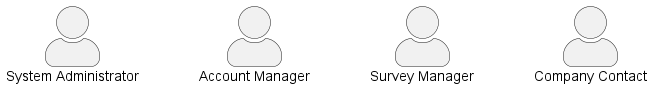
\includegraphics[width=1\textwidth]{images/out/diagrams/actors/actors/actors.png}}
    \caption{Actors Diagram}
    \label{fig:actors_diagram}
\end{figure}

The roles, descriptions, and associated tasks of each actor are summarized in the table below:

\begin{table}[H]
\centering
\caption{Actor Roles and Associated Tasks}
\vspace{0.3cm}
\renewcommand{\arraystretch}{1.4}
\begin{tabular}{|>{\centering\arraybackslash}m{3.2cm}|>{\centering\arraybackslash}m{5.5cm}|m{6.3cm}|}
\hline
\textbf{Actor} & \textbf{Role Description} & \textbf{Associated Tasks} \\ \hline
\textbf{System Administrator} & Configures global parameters, manages administrative accounts, company profiles, and reviews audit logs. & 
$\bullet$ Login \newline
$\bullet$ Manage admins \newline
$\bullet$ Manage locked accounts \newline
$\bullet$ Manage companies \newline
$\bullet$ Manage profile \newline
$\bullet$ Manage system settings \newline
$\bullet$ Receive notifications \newline
$\bullet$ Consult system audit logs \\ \hline
\textbf{Account Manager} & Manages directory data, and representative contacts. & 
$\bullet$ Login \newline
$\bullet$ Manage contacts \newline
$\bullet$ Manage locked accounts \newline
$\bullet$ Manage profile \newline
$\bullet$ Receive notifications \\ \hline
\textbf{Survey Manager} & Manages surveys and passages, uploads PDF questionnaires, and tracks response progress. & 
$\bullet$ Login \newline
$\bullet$ Manage surveys \newline
$\bullet$ Manage profile \newline
$\bullet$ Receive notifications \\ \hline
\textbf{Company Contact} & Represents external entities and accesses assignments. & 
$\bullet$ Login \newline
$\bullet$ Manage profile \newline
$\bullet$ Consult assigned surveys \newline
$\bullet$ Consult assigned results \newline
$\bullet$ Receive notifications \\ \hline
\end{tabular}
\end{table}

\section{Global Use Case Diagram}
The global use case diagram illustrates actor interactions across platform functional boundaries:

\begin{figure}[H]
    \centering
    \makebox[\textwidth][c]{
\includegraphics[width=1\textwidth]{images/out/diagrams/use case/global_use_case/diagram class general3.png}}
    \caption{Global Use Case Diagram}
    \label{fig:global_use_case}
\end{figure}

\section{Product Backlog}
The Product Backlog lists user stories mapped to priorities:

\begin{table}[H]
\centering
\caption{Product Backlog User Stories}
\vspace{0.2cm}
\renewcommand{\arraystretch}{1.15}
\begin{tabular}{|c|p{9.5cm}|c|c|}
\hline
\textbf{ID} & \textbf{User Story} & \textbf{Priority} & \textbf{Sprint} \\ \hline
US01 & As a user, I want to Login to access my secure workspace. & 1 & 0 \\ \hline
US02 & As a System Administrator, I want to Manage admins to set up administrative user accounts. & 1 & 0 \\ \hline
US03 & As a System Administrator or Account Manager, I want to Manage contacts to assign representatives to surveyed companies. & 1 & 0 \\ \hline
US04 & As a System Administrator, I want to Manage companies to maintain business registry files. & 1 & 0 \\ \hline
US05 & As a System Administrator or Survey Manager, I want to Manage surveys to configure survey passages and upload reference forms. & 1 & 0 \\ \hline
US06 & As a Company Contact, I want to Consult assigned surveys to view my active questionnaires. & 2 & 1 \\ \hline
US07  & As a Company Contact, I want to Consult assigned results to check my past survey responses. & 2 & 1 \\ \hline
US08 & As a System Administrator, I want to Manage system settings to configure global parameters. & 2 & 1 \\ \hline
US09  & As a System Administrator or Account Manager, I want to Manage locked accounts to restore or restrict system access. & 2 & 1 \\ \hline
US10 & As a user, I want to Manage profile to modify my personal contact information. & 3 & 1 \\ \hline
US11 & As a user, I want to Receive notifications when relevant platform updates or survey submissions occur. & 2 & 2 \\ \hline
US12 & As a System Administrator, I want to Consult system audit logs to audit system activities. & 2 & 2 \\ \hline
\end{tabular}
\end{table}

\section{Work Environment}

\subsection{Design Methodology}
The project was designed using the \textbf{Agile Scrum Methodology} \cite{scrum}. This choice is motivated by the need for iterative feedback and incremental releases, enabling rapid integration tests between the backend API and the external systems. 
Development was organized into Sprints of two weeks each:
\begin{itemize}
    \item \textbf{Sprint 0:} Backend database setup, authentication, and core administration for Login, Manage admins, Manage contacts, Manage companies, and Manage surveys.
    \item \textbf{Sprint 1:} Frontend portal interface integration, and configuration of Consult assigned surveys, Consult assigned results, Manage system settings, Manage locked accounts, and Manage profile.
    \item \textbf{Sprint 2:} System integration webhooks, Receive notifications engine, Consult system audit logs, and testing.
\end{itemize}

\subsection{Software Environment}
Various software tools, frameworks, and packages were utilized during the design and development of the platform. These tools are grouped into the following categories:

\subsubsection{Development Tools}
The table below lists the primary development tools used to build the application:
\begin{table}[H]
\centering
\caption{Development Tools}
\vspace{0.3cm}
\renewcommand{\arraystretch}{1.3}
\begin{tabular}{|>{\centering\arraybackslash}m{3.5cm}|>{\centering\arraybackslash}m{12.0cm}|}
\hline

\includegraphics[width=3.0cm]{images/logos/logo_vscode.png} & \textbf{Visual Studio Code}: Code editor used for writing Python backend services and TypeScript Angular components. \cite{vscode} \\ \hline

\includegraphics[width=3.0cm]{images/logos/logo_angular.png} & \textbf{Angular}: Single-Page Application (SPA) framework used to develop the responsive administration portal and contact dashboards. \cite{angular} \\ \hline

\includegraphics[width=3.0cm]{images/logos/logo_fastapi.png} & \textbf{FastAPI}: Modern, high-performance web framework for Python used to create the REST API endpoints. \cite{fastapi} \\ \hline

\includegraphics[width=3.0cm]{images/logos/logo_python.png} & \textbf{Python}: Main programming language used to implement the backend business logic and database queries. \cite{python} \\ \hline
\end{tabular}
\end{table}

\subsubsection{Database Tools}
The database backend consists of the following data management tools:
\begin{table}[H]
\centering
\caption{Database Tools}
\vspace{0.3cm}
\renewcommand{\arraystretch}{1.3}
\begin{tabular}{|>{\centering\arraybackslash}m{3.5cm}|>{\centering\arraybackslash}m{12.0cm}|}
\hline

\includegraphics[width=3.0cm]{images/logos/logo_mysql.png} & \textbf{MySQL}: Relational database system utilized through the local XAMPP environment to store secure user records, company profiles, and survey assignments. \cite{mysql} \\ \hline

\includegraphics[width=3.0cm]{images/logos/logo_sqlite.png} & \textbf{SQLite}: Lightweight database engine utilized in development for rapid testing and zero-configuration local database initialization. \cite{sqlite} \\ \hline
\end{tabular}
\end{table}

\newpage
\subsubsection{Background Processing \& Libraries}
The background task workers and helper libraries used to optimize platform workflows are listed below:
\begin{table}[H]
\centering
\caption{Task Queues and Libraries}
\vspace{0.3cm}
\renewcommand{\arraystretch}{1.3}
\begin{tabular}{|>{\centering\arraybackslash}m{3.5cm}|>{\centering\arraybackslash}m{12.0cm}|}
\hline

\includegraphics[width=3.0cm]{images/logos/logo_celery.png} & \textbf{Celery}: Distributed task queue used to run asynchronous background operations. \cite{celery} \\ \hline

\includegraphics[width=3.0cm]{images/logos/logo_redis.png} & \textbf{Redis}: High-performance in-memory data store utilized as the message broker for Celery queues. \cite{redis} \\ \hline

\includegraphics[width=3.0cm]{images/logos/logo_docker.png} & \textbf{Docker}: Containerization platform used to deploy Redis as an isolated, reproducible container during development. \cite{docker} \\ \hline

\includegraphics[width=3.0cm]{images/logos/logo_python.png} & \textbf{SQLAlchemy}: Object-Relational Mapper (ORM) used to map Python models to SQL database tables securely. \cite{sqlalchemy} \\ \hline

\includegraphics[width=3.0cm]{images/logos/logo_ngx_translate.png} & \textbf{NGX-Translate}: Internationalization (i18n) library for Angular used to enable dynamic multi-language UI translation (Arabic, French, English) via asynchronous JSON translation loaders. \cite{ngx_translate} \\ \hline
\end{tabular}
\end{table}

To prevent synchronous blocking of the main web server and ensure full multi-language accessibility, the platform architecture incorporates dedicated asynchronous background processing and client-side internationalization layers:

\begin{enumerate}
    \item \textbf{Dual Role of Redis:}
    Redis \cite{redis} operates in a dual capacity within the platform. First, it serves as the high-throughput \textbf{Message Broker} that holds queued tasks waiting for execution by background workers. Second, it acts as a volatile \textbf{Security \& Session In-Memory Cache}, storing short-lived security tokens such as 2FA OTP codes with dynamic Time-To-Live (TTL) expirations, login rate-limiting counters, and account lockout tracking flags.
    
    \item \textbf{Celery Task Worker Pipeline:}
    Celery \cite{celery} is integrated alongside FastAPI to decouple I/O-heavy and computationally intensive operations from the synchronous HTTP request-response cycle. By delegating long-running tasks—such as parsing large company sample Excel files, dispatching batch email notifications, and generating audit log exports—to a multi-threaded worker pool, the primary API maintains near-zero latency and remains completely responsive to concurrent user requests.

    \item \textbf{NGX-Translate Internationalization Engine:}
    NGX-Translate \cite{ngx_translate} is integrated into the Angular Single-Page Application to deliver dynamic, client-side multi-language translation (Arabic, French, and English). Utilizing \texttt{TranslateHttpLoader}, the engine asynchronously fetches localized JSON dictionary assets (\texttt{fr.json}, \texttt{ar.json}, \texttt{en.json}) upon application initialization or language switching. The framework injects translations seamlessly into UI templates via RxJS streams and Angular pipes, guaranteeing full internationalization (i18n) support across all administrative and contact dashboards without requiring page reloads or backend rendering overhead. Furthermore, full Right-to-Left (RTL) layout mirroring is dynamically applied to component containers and CSS input properties via Angular \texttt{[dir]="currentLang() === 'ar' ? 'rtl' : 'ltr'"} bindings whenever Arabic is selected, ensuring fluent bidirectionality across LTR and RTL scripts.
\end{enumerate}

\subsubsection{Testing and Validation Tools}
The API testing and interface verification was performed using the following tool:
\begin{table}[H]
\centering
\caption{Testing Tools}
\vspace{0.3cm}
\renewcommand{\arraystretch}{1.3}
\begin{tabular}{|>{\centering\arraybackslash}m{3.5cm}|>{\centering\arraybackslash}m{12.0cm}|}
\hline

\includegraphics[width=3.0cm]{images/logos/logo_postman.png} & \textbf{Postman}: API client platform used to construct, document, and test backend REST endpoints and webhook payloads. \cite{postman} \\ \hline
\end{tabular}
\end{table}

\subsubsection{Conception and Modeling Tools}
The conceptual structure and diagrams of the system were designed using the following tool:
\begin{table}[H]
\centering
\caption{Conception and Modeling Tools}
\vspace{0.3cm}
\renewcommand{\arraystretch}{1.3}
\begin{tabular}{|>{\centering\arraybackslash}m{3.5cm}|>{\centering\arraybackslash}m{12.0cm}|}
\hline

\includegraphics[width=3.0cm]{images/logos/logo_plantuml.png} & \textbf{PlantUML}: Open-source modeling tool used to define and generate UML use case diagrams, sequence diagrams, and class diagrams from plain text descriptions. \cite{plantuml} \\ \hline
\end{tabular}
\end{table}

\subsubsection{Collaboration Tools}
To organize version branches and documents during development, the following tools were used:
\begin{table}[H]
\centering
\caption{Collaboration Tools}
\vspace{0.3cm}
\renewcommand{\arraystretch}{1.3}
\begin{tabular}{|>{\centering\arraybackslash}m{3.5cm}|>{\centering\arraybackslash}m{12.0cm}|}
\hline

\includegraphics[width=3.0cm]{images/logos/logo_git.png} & \textbf{Git}: Distributed version control system used to track source code edits. \cite{git} \\ \hline

\includegraphics[width=3.0cm]{images/logos/logo_github.png} & \textbf{GitHub}: Repository hosting service used to push code versions, manage pull requests, and review commits. \cite{github} \\ \hline

\includegraphics[width=3.0cm]{images/logos/logo_overleaf.png} & \textbf{Overleaf}: Online LaTeX editor used for collaborative writing and document compilation of this report. \cite{overleaf} \\ \hline
\end{tabular}
\end{table}

\section{Conclusion}
This chapter defined the Requirements Specification of the INS Statistical Survey Collection Platform. We detailed the system context, identified functional and non-functional requirements, mapped user roles, presented the product backlog, and outlined the Scrum methodology and software environment. The next chapter will present the first development sprint covering authentication and core administrative features.

% ============================================================
% CHAPTER 3 - SPRINT 0: AUTHENTICATION & ADMINISTRATIVE CORE
% ============================================================
\chapter{Sprint 0 -- Authentication \& Administrative Core}

\section{Introduction}
In this chapter, we present the first sprint of the project, which covers the foundational authentication and administrative core features. The study of this sprint encompasses backlog identification, use case refinement, system conception, and user interface implementation.

Sprint 0 focuses on establishing secure user authentication, role-based access control, and administrative management of users, contacts, company registries, and survey campaign configurations. These features provide the core operational foundation upon which subsequent survey management sprints are constructed.

\section{Sprint 0 Backlog Identification}
The sprint backlog contains all User Stories selected from the Product Backlog for Sprint 0. Each story follows the "INVEST" criteria (Independent, Negotiable, Valuable, Estimable, Small, Testable). Table \ref{tab:sprint0_backlog} outlines the user stories prioritized for Sprint 0:

\begin{table}[H]
\centering
\caption{Sprint 0 Backlog -- Authentication \& Administrative Core}
\label{tab:sprint0_backlog}
\vspace{0.3cm}
\renewcommand{\arraystretch}{1.3}
\begin{tabular}{|c|p{9.5cm}|c|}
\hline
\textbf{ID} & \textbf{User Story} & \textbf{Estimation} \\ \hline
US01 & As a user, I want to Login to access my secure workspace. & High \\ \hline
US02 & As a System Administrator, I want to Manage admins to set up administrative user accounts. & Medium \\ \hline
US03 & As a System Administrator or Account Manager, I want to Manage contacts to assign representatives to surveyed companies. & Medium \\ \hline
US04 & As a System Administrator, I want to Manage companies to maintain business registry files. & High \\ \hline
US05 & As a System Administrator or Survey Manager, I want to Manage surveys to configure survey passages and upload reference forms. & High \\ \hline
\end{tabular}
\end{table}

A User Story in Sprint 0 is considered "completed" when:
\begin{itemize}
    \item Frontend UI components and backend REST API endpoints are developed and integrated.
    \item Input validation, password hashing, and token handling are verified.
    \item Core functionality and REST endpoints are manually verified via Postman collections and technical documentation is updated.
\end{itemize}

\section{Sprint 0 Refinement}
In this section, we refine the functional details and textual specifications for the following four use cases:
\begin{itemize}
    \item Login;
    \item Manage admins;
    \item Manage contacts;
    \item Manage companies;
    \item Manage surveys.
\end{itemize}
\newpage
\subsection{Refinement of the Use Case ``Login''}
The diagram below illustrates the refinement of the ``Login'' use case and its interactions with system actors:

\begin{figure}[H]
    \centering
    \makebox[\textwidth][c]{
\includegraphics[width=1\textwidth]{images/out/diagrams/use case/login.png}}
    \caption{Refinement of the use case ``Login''}
    \label{fig:refinement_login}
\end{figure}
    Table \ref{tab:refinement_login} presents the textual description of the ``Login'' use case:

\begin{table}[H]
\centering
\caption{Textual description -- Login}
\label{tab:refinement_login}
\vspace{0.2cm}
\small
\renewcommand{\arraystretch}{1.1}
\begin{tabular}{|p{3.5cm}|p{12.0cm}|}
\hline
\textbf{Use Case} & Login \\ \hline
\textbf{Actor} & System Administrator, Account Manager, Survey Manager, Company Contact \\ \hline
\textbf{Pre-condition} & The user has registered credentials or an active account in the system database. \\ \hline
\textbf{Post-condition} & The user is authenticated, passes OTP verification, completes initial password setup if first-time user, is redirected to their role dashboard, and the login event is recorded in the system audit logs. \\ \hline
\textbf{Main Scenario} & 
1. The user navigates to the login interface. \newline
2. The system presents the authentication form (email and password). \newline
3. The user submits their credentials. \newline
4. The system validates credentials against database records (bcrypt password verification). \newline
5. The system generates a One-Time Password (OTP) code, stores it in an in-memory Redis data store \cite{redis} with a dynamic expiration TTL configured via global system settings, and dispatches it to the user's registered email address. \newline
6. The system presents the OTP verification interface. \newline
7. The user enters the received OTP code and submits the form. \newline
8. The system verifies the submitted OTP code against the Redis store \cite{redis}. \newline
9. If it is the user's first time logging in, the system redirects them to the password reset page; otherwise, the system issues an authentication payload (JWT token) and redirects them to their role-specific dashboard. \newline
10. The system creates an audit log entry recording the user authentication event (user ID, timestamp, IP address, and status). \\ \hline
\textbf{Alternative Scenarios} & 
$\bullet$ Invalid credentials: The system records a failed login attempt in the audit logs and displays an error message indicating invalid email or password. \newline
$\bullet$ Invalid or expired OTP: The system displays an error message and prompts the user to request a new OTP code. \newline
$\bullet$ First-time login password change incomplete: The system restricts workspace access until a new password is set. \newline
$\bullet$ Locked account: The system notifies the user that their account is locked and directs them to an administrator. \\ \hline
\textbf{Exception} & Database or mail server connection failure; the system displays a server error notification. \\ \hline
\end{tabular}
\end{table}

\subsection{Refinement of the Use Case ``Manage admins''}
The diagram below illustrates the refinement of the ``Manage admins'' use case and its interactions with system actors:

\begin{figure}[H]
    \centering
    \makebox[\textwidth][c]{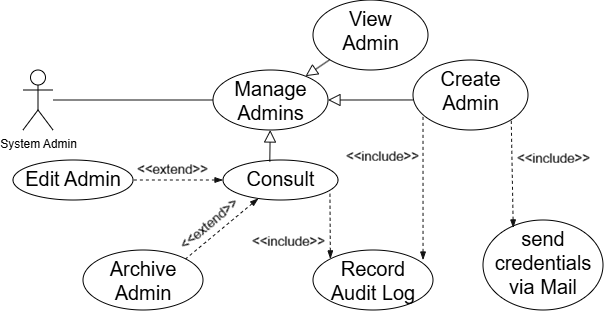
\includegraphics[width=1\textwidth]{images/out/diagrams/use case/manage_admins.png}}
    \caption{Refinement of the use case ``Manage admins''}
    \label{fig:refinement_manage_admins}
\end{figure}
\newpage
Table \ref{tab:refinement_manage_admins} presents the textual description of the ``Manage admins'' use case:

\begin{table}[H]
\centering
\caption{Textual description -- Manage admins}
\label{tab:refinement_manage_admins}
\vspace{0.2cm}
\small
\renewcommand{\arraystretch}{1.15}
\begin{tabular}{|p{3.5cm}|p{12.0cm}|}
\hline
\textbf{Use Case} & Manage admins \\ \hline
\textbf{Actor} & System Administrator \\ \hline
\textbf{Pre-condition} & The System Administrator is authenticated with active super-admin privileges. \\ \hline
\textbf{Post-condition} & Administrative accounts are created, updated, or archived in the database, initial credentials are sent to the new administrator via email, and the administrative action is recorded in the system audit logs. \\ \hline
\textbf{Main Scenario} & 
1. The administrator navigates to the admin management dashboard. \newline
2. The system retrieves and displays the table of existing administrative accounts. \newline
3. The administrator selects an action (create new admin, update role/email, or archive account). \newline
4. The administrator fills in the required fields and submits the request. \newline
5. The system validates the input data (format and email uniqueness). \newline
6. The system executes the requested transaction in the database (creating, updating, or archiving the admin account). \newline
7. Upon account creation, the system dispatches an automated email to the new administrator containing their temporary credentials. \newline
8. The system creates an entry in the system audit logs recording the administrative management action (action type, target admin ID, performing admin ID, timestamp, and IP address). \newline
9. The system displays a confirmation notification and updates the account list. \\ \hline
\textbf{Alternative Scenarios} & 
$\bullet$ Duplicate email: The system blocks submission and alerts the administrator. \newline
$\bullet$ Invalid data format: The system highlights invalid fields in the form. \newline
$\bullet$ Mail server error: The system creates the account, logs a notification warning in audit logs, and permits resending credentials. \\ \hline
\textbf{Exception} & Database connection failure; the system displays a generic server error. \\ \hline
\end{tabular}
\end{table}
\newpage
\subsection{Refinement of the Use Case ``Manage contacts''}
The diagram below illustrates the refinement of the ``Manage contacts'' use case and its interactions with system actors:

\begin{figure}[H]
    \centering
    \makebox[\textwidth][c]{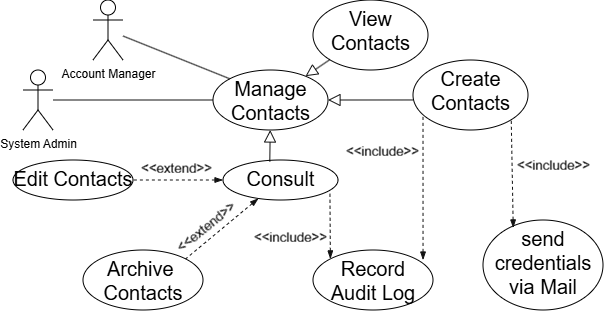
\includegraphics[width=1\textwidth]{images/out/diagrams/use case/account_manager.png}}
    \caption{Refinement of the use case ``Manage contacts''}
    \label{fig:refinement_manage_contacts}
\end{figure}
\newpage
Table \ref{tab:refinement_manage_contacts} presents the textual description of the ``Manage contacts'' use case:

\begin{table}[H]
\centering
\caption{Textual description -- Manage contacts}
\label{tab:refinement_manage_contacts}
\vspace{0.2cm}
\small
\renewcommand{\arraystretch}{1.15}
\begin{tabular}{|p{3.5cm}|p{12.0cm}|}
\hline
\textbf{Use Case} & Manage contacts \\ \hline
\textbf{Actor} & System Administrator, Account Manager \\ \hline
\textbf{Pre-condition} & The user is logged in with System Administrator or Account Manager role privileges. \\ \hline
\textbf{Post-condition} & Company contact records are created, linked to targeted companies, updated, or enabled/disabled in the database, initial access credentials are sent to the contact via email, and the action is recorded in the system audit logs. \\ \hline
\textbf{Main Scenario} & 
1. The manager accesses the contact directory interface. \newline
2. The system displays company contacts filtered by search or company criteria. \newline
3. The manager selects an action (add contact, assign to company, edit contact details, or disable/enable contact). \newline
4. The manager submits the contact profile form. \newline
5. The system validates contact phone, email, and company association. \newline
6. The system updates database records (creating, updating, linking, or disabling/enabling the contact profile). \newline
7. Upon contact creation or assignment, the system dispatches an automated email to the contact containing their initial login credentials. \newline
8. The system creates an entry in the system audit logs recording the contact management action (action type, target contact ID, performing user ID, timestamp, and IP address). \newline
9. The system confirms successful operation and updates the contact directory view. \\ \hline
\textbf{Alternative Scenarios} & 
$\bullet$ Unassigned company: The system prompts the manager to select a valid registered company. \newline
$\bullet$ Form validation errors: The system prevents saving until all mandatory contact fields are valid. \newline
$\bullet$ Mail server error: The system saves the contact profile, logs a notification warning in audit logs, and permits re-inviting the contact. \\ \hline
\textbf{Exception} & Server connection drop; the system displays a network retry prompt. \\ \hline
\end{tabular}
\end{table}
\newpage
\subsection{Refinement of the Use Case ``Manage companies''}
The diagram below illustrates the refinement of the ``Manage companies'' use case and its interactions with system actors:

\begin{figure}[H]
    \centering
    \makebox[\textwidth][c]{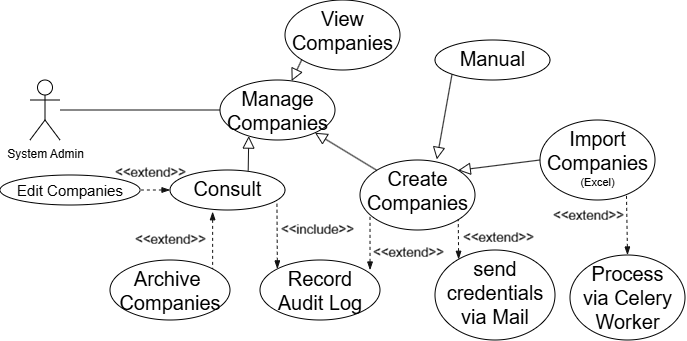
\includegraphics[width=1\textwidth]{images/out/diagrams/use case/manage_companies.png}}
    \caption{Refinement of the use case ``Manage companies''}
    \label{fig:refinement_manage_companies}
\end{figure}

Table \ref{tab:refinement_manage_companies} presents the textual description of the ``Manage companies'' use case:

\begin{table}[H]
\centering
\caption{Textual description -- Manage companies}
\label{tab:refinement_manage_companies}
\vspace{0.2cm}
\small
\renewcommand{\arraystretch}{1.15}
\begin{tabular}{|p{3.5cm}|p{12.0cm}|}
\hline
\textbf{Use Case} & Manage companies \\ \hline
\textbf{Actor} & System Administrator \\ \hline
\textbf{Pre-condition} & The System Administrator is authenticated on the platform with administrative privileges. \\ \hline
\textbf{Post-condition} & Company records are created, updated, imported, or archived in the database, bulk Excel imports are parsed asynchronously via Celery background workers \cite{celery}, and the action is recorded in the system audit logs. \\ \hline
\textbf{Main Scenario} & 
1. The administrator opens the company registry management interface. \newline
2. The system presents the company directory with search and filter capabilities. \newline
3. The administrator selects an action (manually add a company, edit company details, archive a company, or batch import companies via Excel file). \newline
4. \textbf{Manual Entry:} The administrator enters or updates company fields (tax ID / NIS code, legal name, sector, address); the system validates and commits database changes. \newline
5. \textbf{Excel Batch Import:} The administrator selects and uploads an Excel file (.xlsx / .xls) containing company rows. \newline
6. The system validates the file structure and offloads parsing to an asynchronous Celery worker \cite{celery} via Redis broker \cite{redis} to prevent API blocking. \newline
7. The Celery worker parses the file in the background, validates each row, creates or updates company records, and records parsing status. \newline
8. The system dispatches an in-app notification summarizing import results (inserted rows, updated rows, and error count). \newline
9. The system creates an entry in the system audit logs recording the company management or batch import action (performing admin ID, timestamp, processed row count, and status). \newline
10. The system displays a success message and refreshes the company directory. \\ \hline
\textbf{Alternative Scenarios} & 
$\bullet$ Duplicate tax ID / NIS code: The system rejects manual creation or flags the duplicate row during batch import. \newline
$\bullet$ Invalid Excel file structure: The system blocks upload and alerts the administrator to check mandatory column headers. \newline
$\bullet$ Partial batch import errors: Celery processes valid rows, logs bad rows, and attaches an error report to the summary notification. \\ \hline
\textbf{Exception} & Database or background task queue connection failure; the system logs the failure in audit logs and displays an error message. \\ \hline
\end{tabular}
\end{table}

\newpage
\subsection{Refinement of the Use Case ``Manage surveys''}
The diagram below illustrates the refinement of the ``Manage surveys'' use case and its interactions with system actors:

\begin{figure}[H]
    \centering
    \makebox[\textwidth][c]{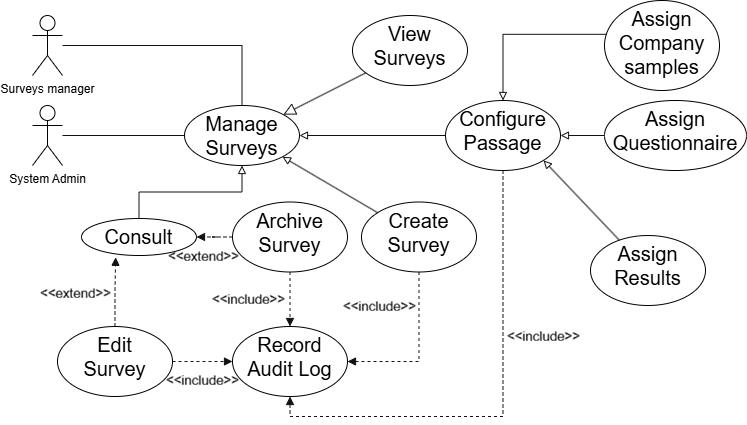
\includegraphics[width=1\textwidth]{images/out/diagrams/use case/manage surveys.png}}
    \caption{Refinement of the use case ``Manage surveys''}
    \label{fig:refinement_manage_surveys}
\end{figure}
\newpage
Table \ref{tab:refinement_manage_surveys} presents the textual description of the ``Manage surveys'' use case:

\begin{table}[H]
\centering
\caption{Textual description -- Manage surveys}
\label{tab:refinement_manage_surveys}
\vspace{0.2cm}
\small
\renewcommand{\arraystretch}{1.15}
\begin{tabular}{|p{3.5cm}|p{12.0cm}|}
\hline
\textbf{Use Case} & Manage surveys \\ \hline
\textbf{Actor} & System Administrator, Survey Manager \\ \hline
\textbf{Pre-condition} & The user is authenticated on the platform with System Administrator or Survey Manager role privileges. \\ \hline
\textbf{Post-condition} & Survey definitions, periodic passages, targeted company samples, and questionnaire reference forms are created, configured, or archived in the database, and recorded in system audit logs. \\ \hline
\textbf{Main Scenario} & 
1. The survey manager navigates to the survey management dashboard. \newline
2. The system displays the directory of statistical survey campaigns. \newline
3. The manager selects a survey campaign and configures its periodic passages (e.g., annual or quarterly survey editions). \newline
4. For each passage, the manager sets passage parameters (passage title, start/end collection dates, statistical domain) and attaches questionnaire reference templates (PDF/Excel). \newline
5. The manager defines and assigns the company sample (targeted list of registered enterprise representatives) for the specific survey passage. \newline
6. The system validates passage dates, company sample selections, and template file formats. \newline
7. The system commits the survey passage and its associated company sample to the database. \newline
8. The system creates an entry in the system audit logs recording the survey passage and sample configuration action (performing user ID, survey ID, passage ID, assigned sample count, timestamp, IP address). \newline
9. The system displays a confirmation notification and updates the survey passage directory. \\ \hline
\textbf{Alternative Scenarios} & 
$\bullet$ Invalid date range: The system alerts the manager if the passage end date precedes the start date. \newline
$\bullet$ Empty company sample: The system warns the manager if no companies are assigned to the passage sample. \newline
$\bullet$ Invalid form file format: The system blocks upload and specifies valid template extensions. \\ \hline
\textbf{Exception} & Database transaction failure; the system rolls back changes and displays an error prompt. \\ \hline
\end{tabular}
\end{table}

\section{Sprint 0 Conception}
This section presents the structural and dynamic design models for the use cases implemented in Sprint 0.

\subsection{Class Diagram -- Sprint 0 Core Domain}
The class diagram models the entity structures, attributes, and relationships supporting authentication and administrative management:

\begin{figure}[H]
    \centering
    \makebox[\textwidth][c]{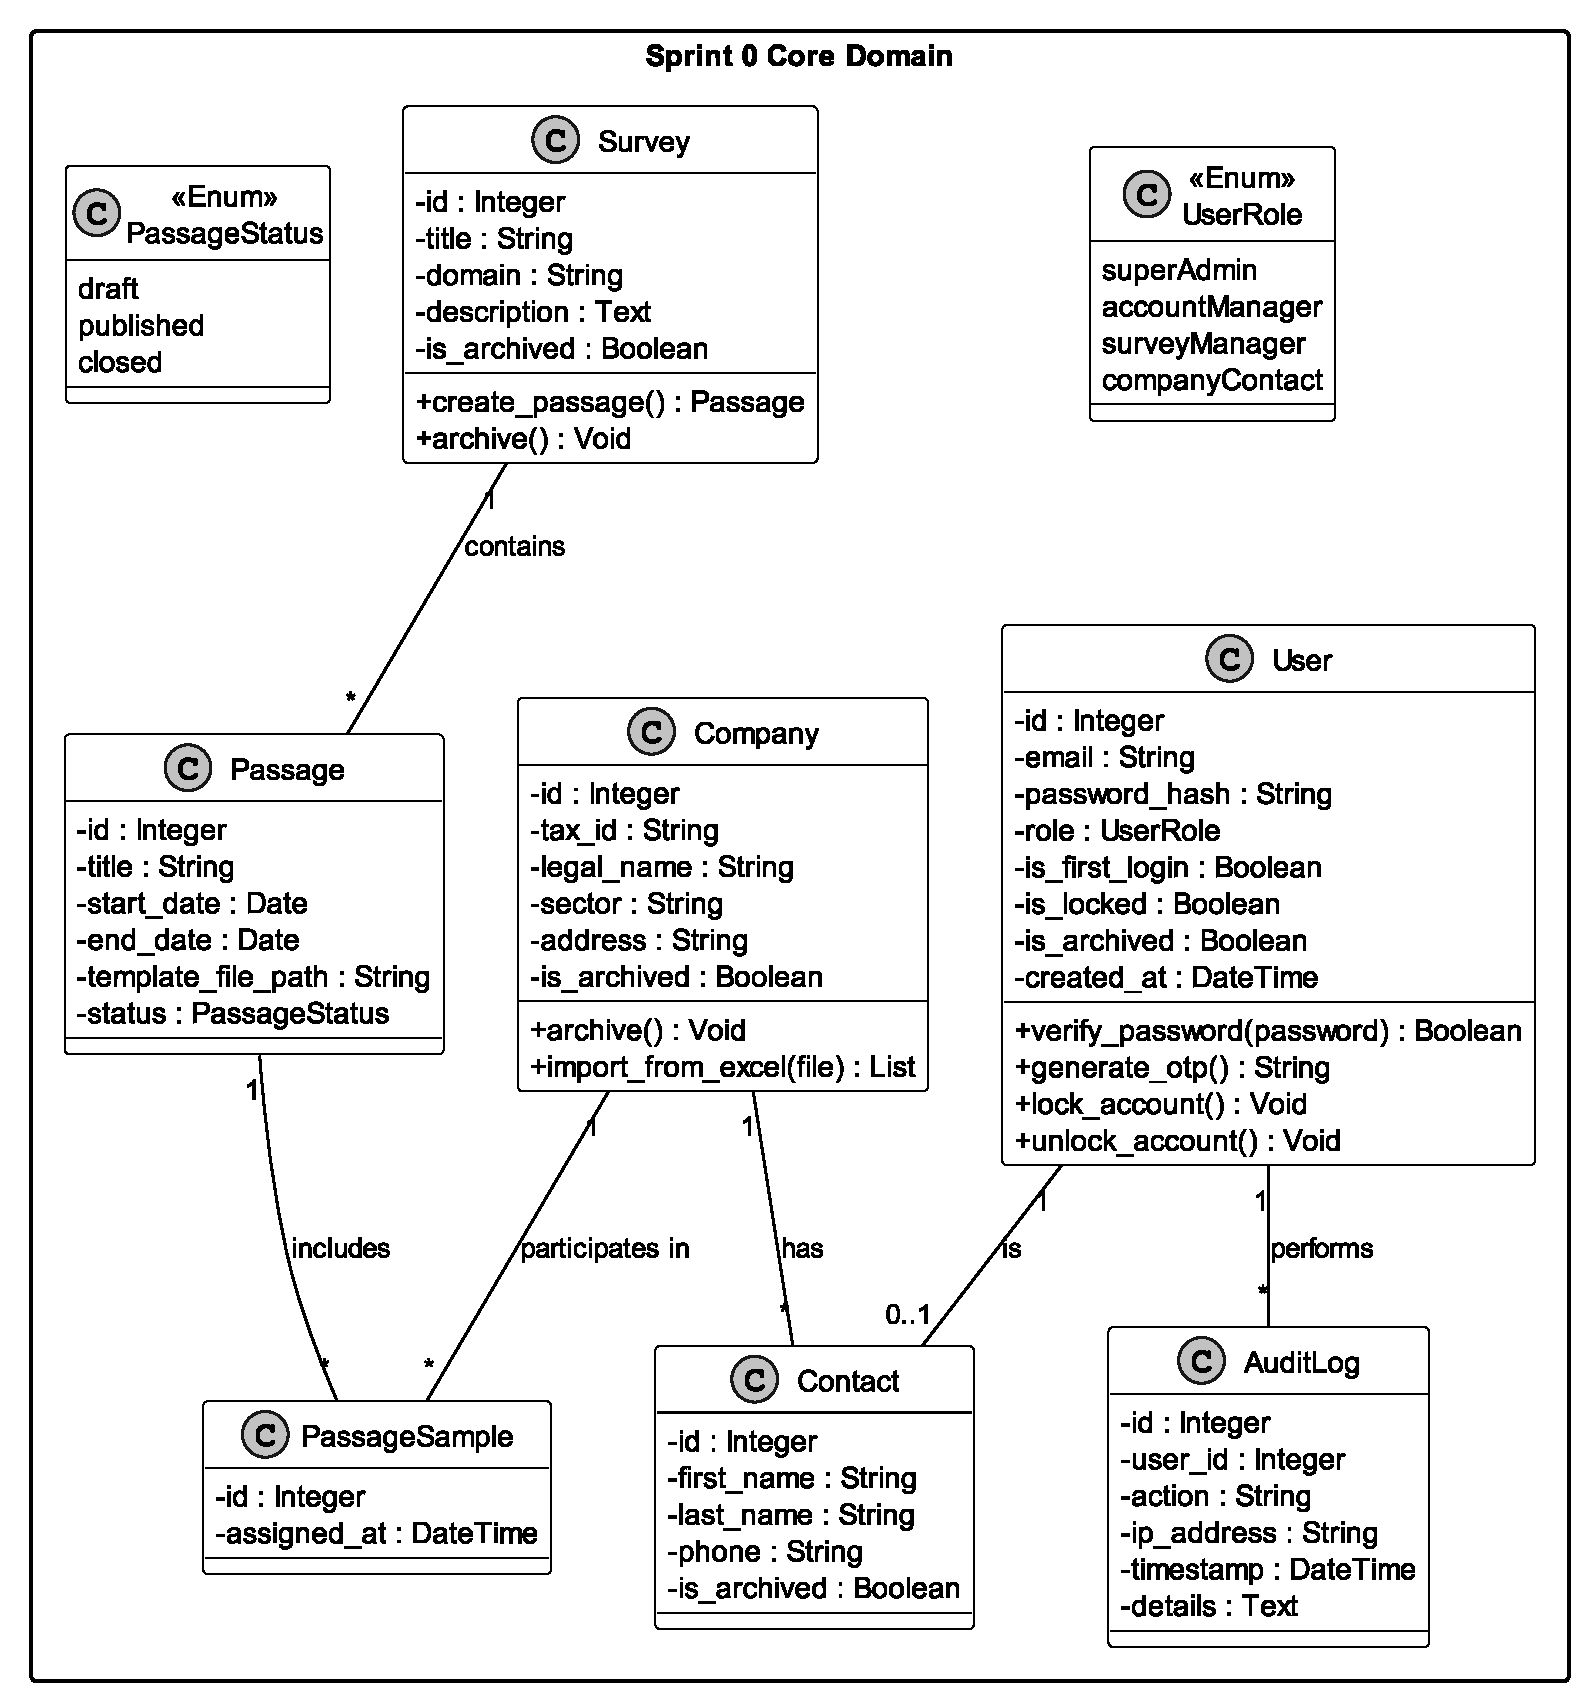
\includegraphics[width=1\textwidth]{images/out/diagrams/class/sprint0/sprint0.eps}}
    \caption{Sprint 0 Class Diagram}
    \label{fig:sprint0_class_diagram}
\end{figure}

The Sprint 0 class diagram (Figure \ref{fig:sprint0_class_diagram}) establishes the structural core of the platform data model. The \texttt{User} entity serves as the primary authentication actor, possessing a foreign key relationship to \texttt{Role} (System Administrator, Account Manager, Survey Manager, Company Contact). The administrative domain connects \texttt{Company} to economic classification entities (\texttt{Sector} and \texttt{Activity}) via foreign keys, establishing normalized company master records. Company contact representatives are modeled through the \texttt{Contact} entity, which establishes a one-to-many relationship with \texttt{Company}. Statistical survey campaigns are modeled by \texttt{Survey}, linked to periodic \texttt{SurveyPassage} instances. Each passage maintains relationships to \texttt{SampleCompany} (the assigned company sample) and \texttt{SurveyQuestionnaire} (reference documents).
\newpage
\subsection{Activity Diagram -- Use Case ``Login''}
The activity diagram below illustrates the decision flows, validations, and branching logic during the login process, including OTP verification and first-time login redirection:

\begin{figure}[H]
    \centering
    \makebox[\textwidth][c]{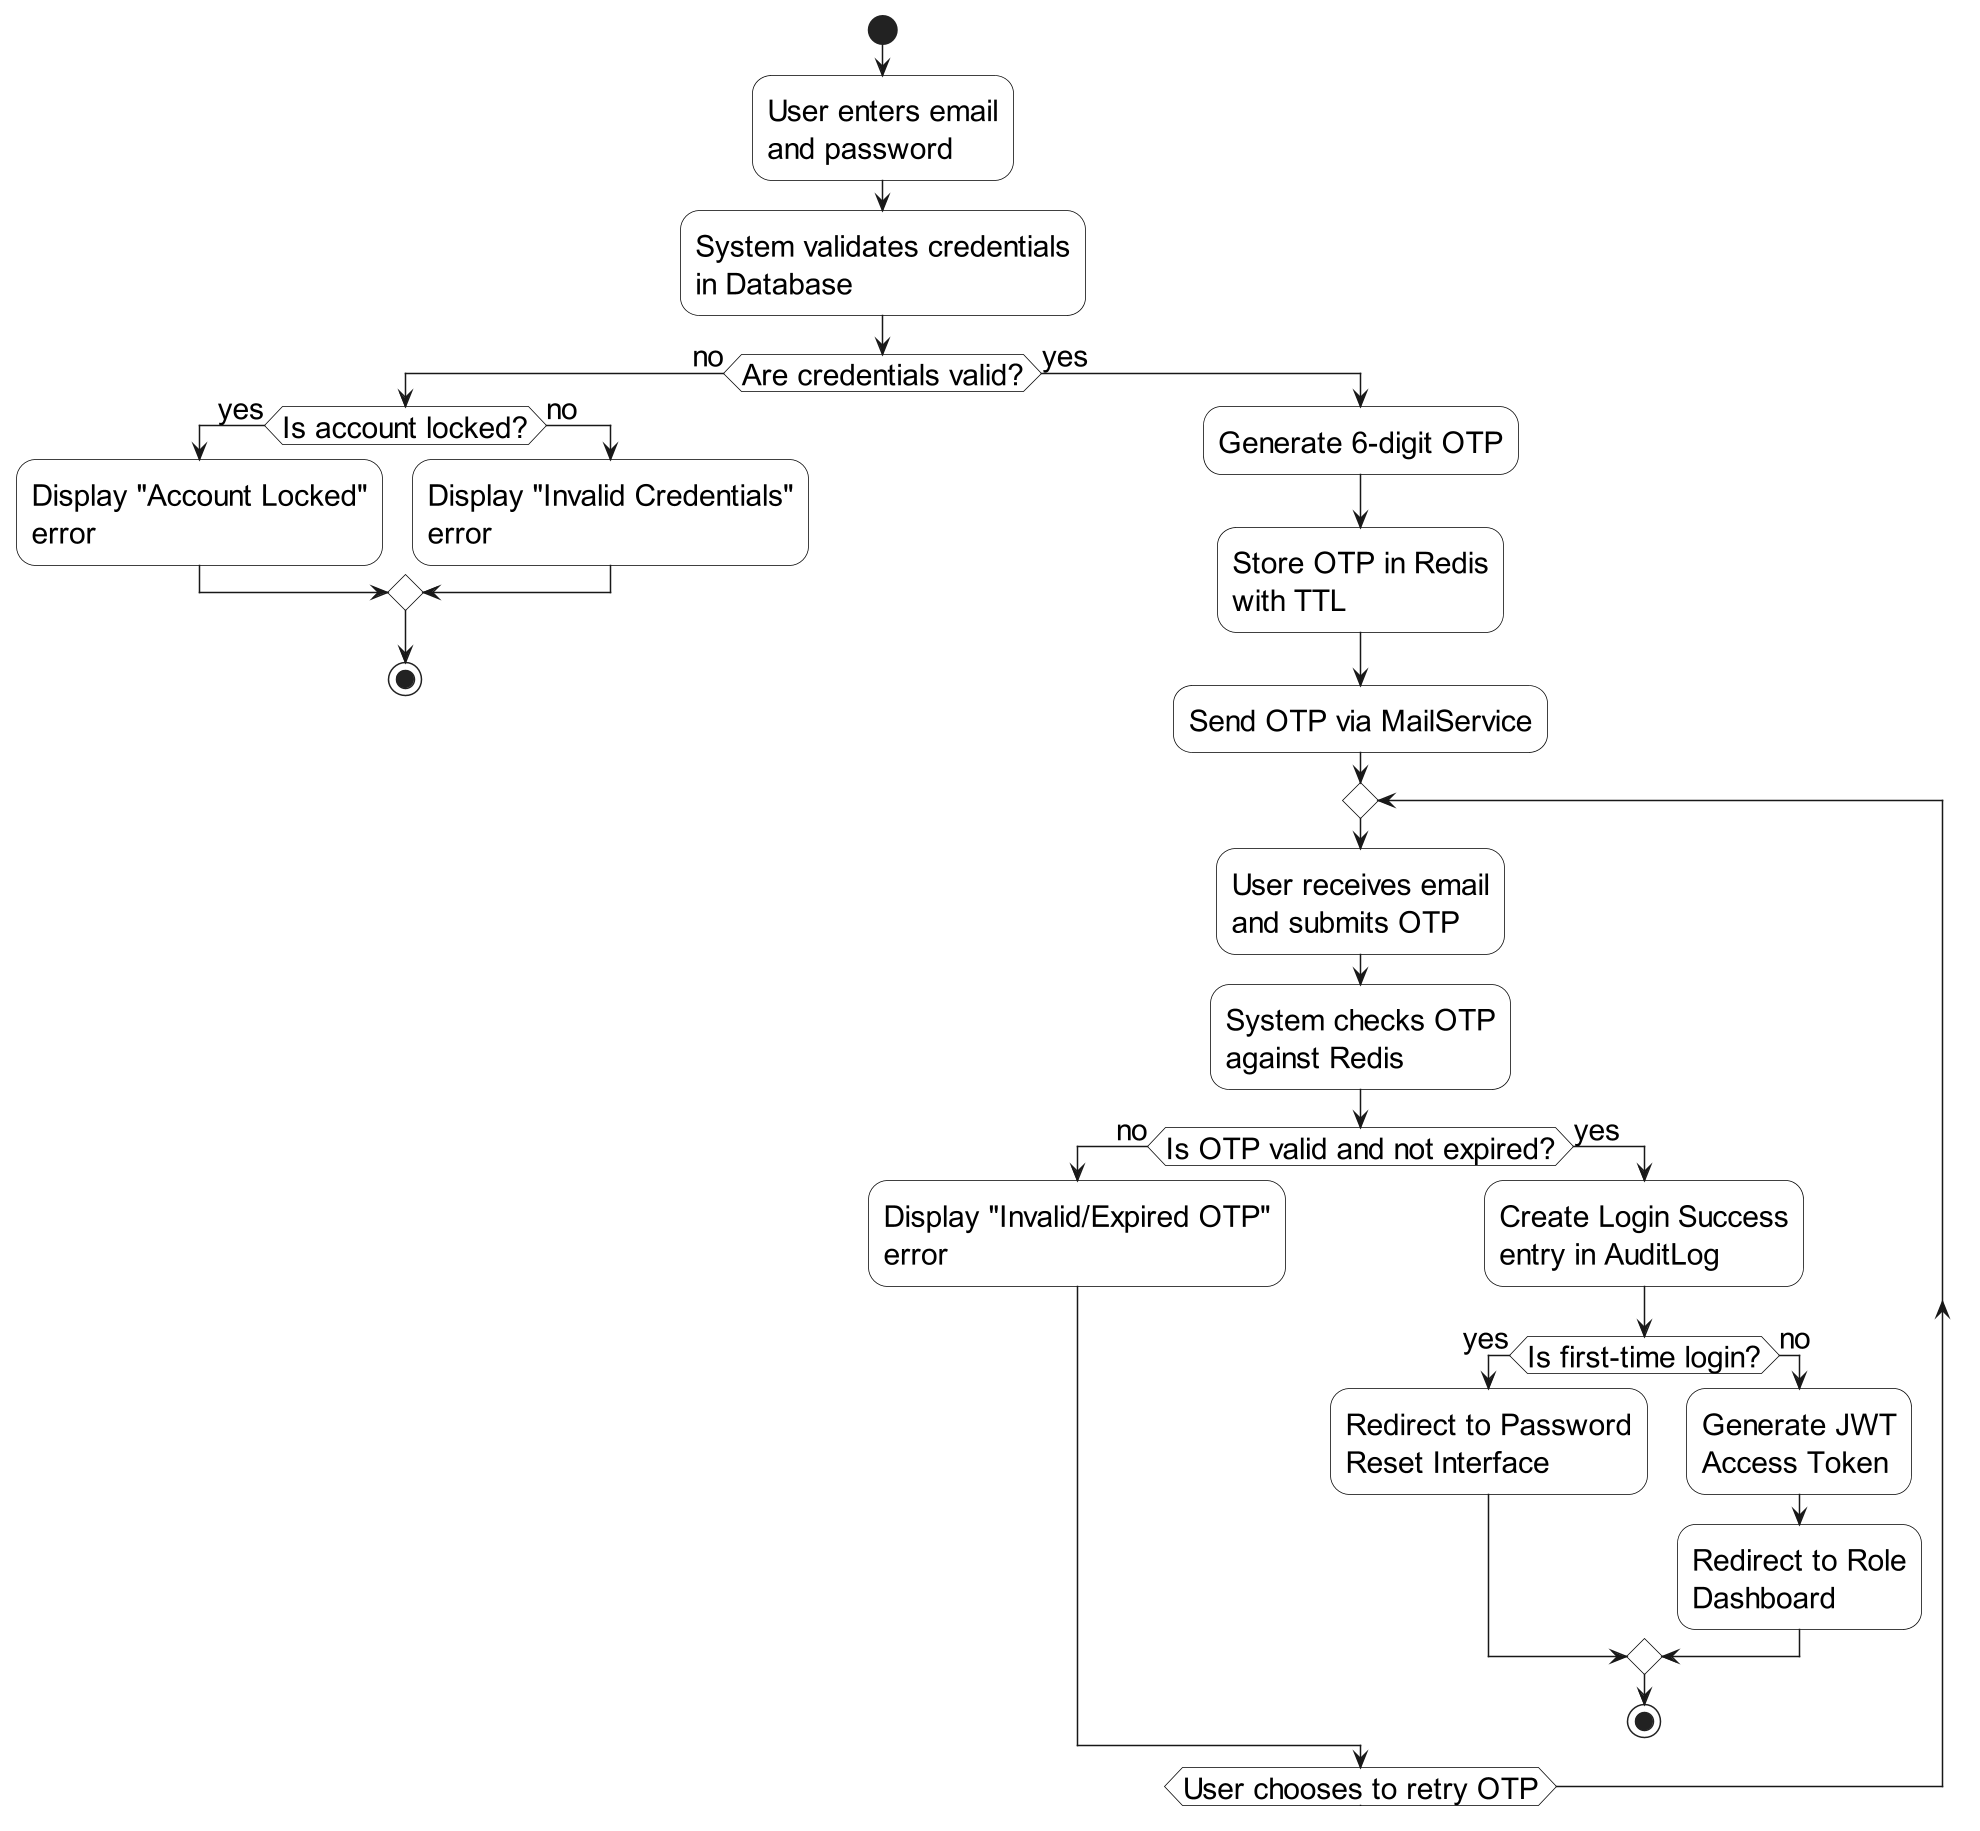
\includegraphics[width=1.4\textwidth,height=0.75\textheight,keepaspectratio]{images/out/diagrams/activite/act_login.png}}
    \caption{Activity Diagram -- Login}
    \label{fig:seq_login}
\end{figure}

\subsection{Sequence Diagram -- Use Case ``Manage admins''}
The sequence diagram below details administrative account creation and management interactions:

\begin{figure}[H]
    \centering
    \makebox[\textwidth][c]{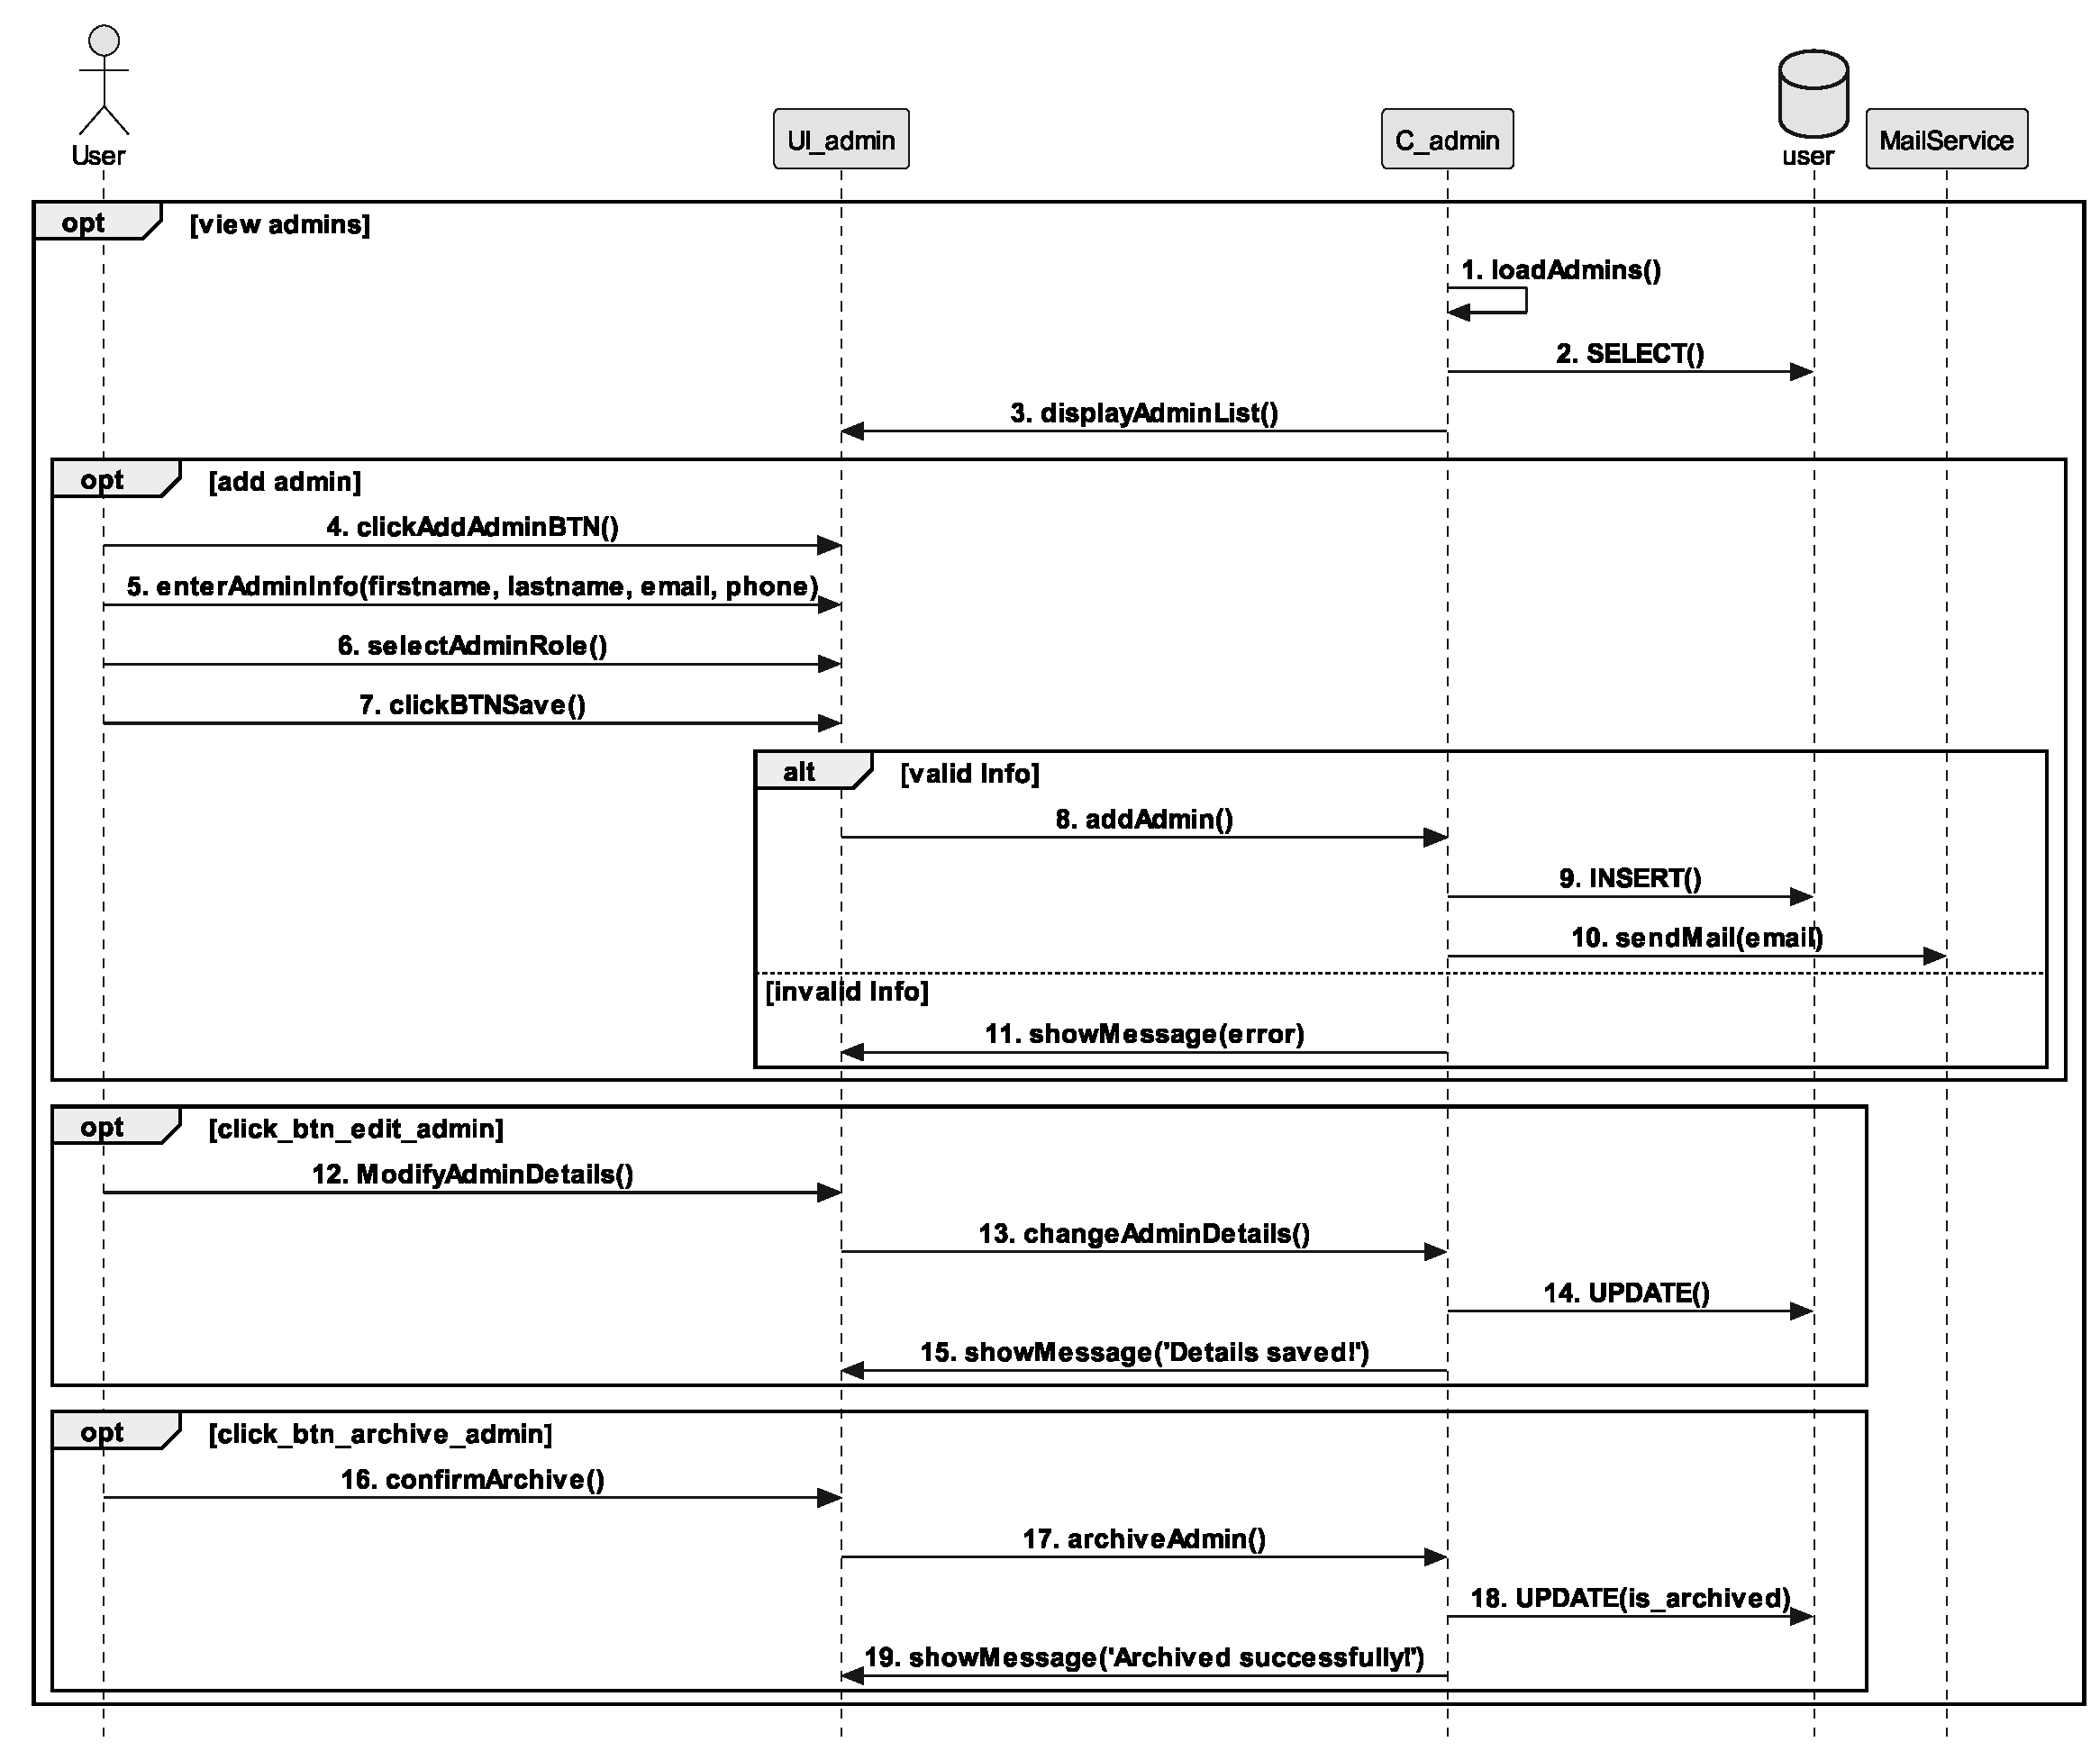
\includegraphics[width=1.2\textwidth]{images/out/diagrams/seq/manage_admin/manage_admin.eps}}
    %\framebox[0.85\linewidth][c]{\parbox{0.85\linewidth}{\centering\vspace{2.5cm}\textbf{Sequence Diagram -- Manage admins Placeholder}\\\textit{(Uncomment line above when image is ready)}\vspace{2.5cm}}}
    \caption{Sequence Diagram -- Manage admins}
    \label{fig:seq_manage_admins}
\end{figure}

\newpage
\subsection{Sequence Diagram -- Use Case ``Manage contacts''}
The sequence diagram below shows contact registration and company assignment interactions:

\begin{figure}[H]
    \centering
    \makebox[\textwidth][c]{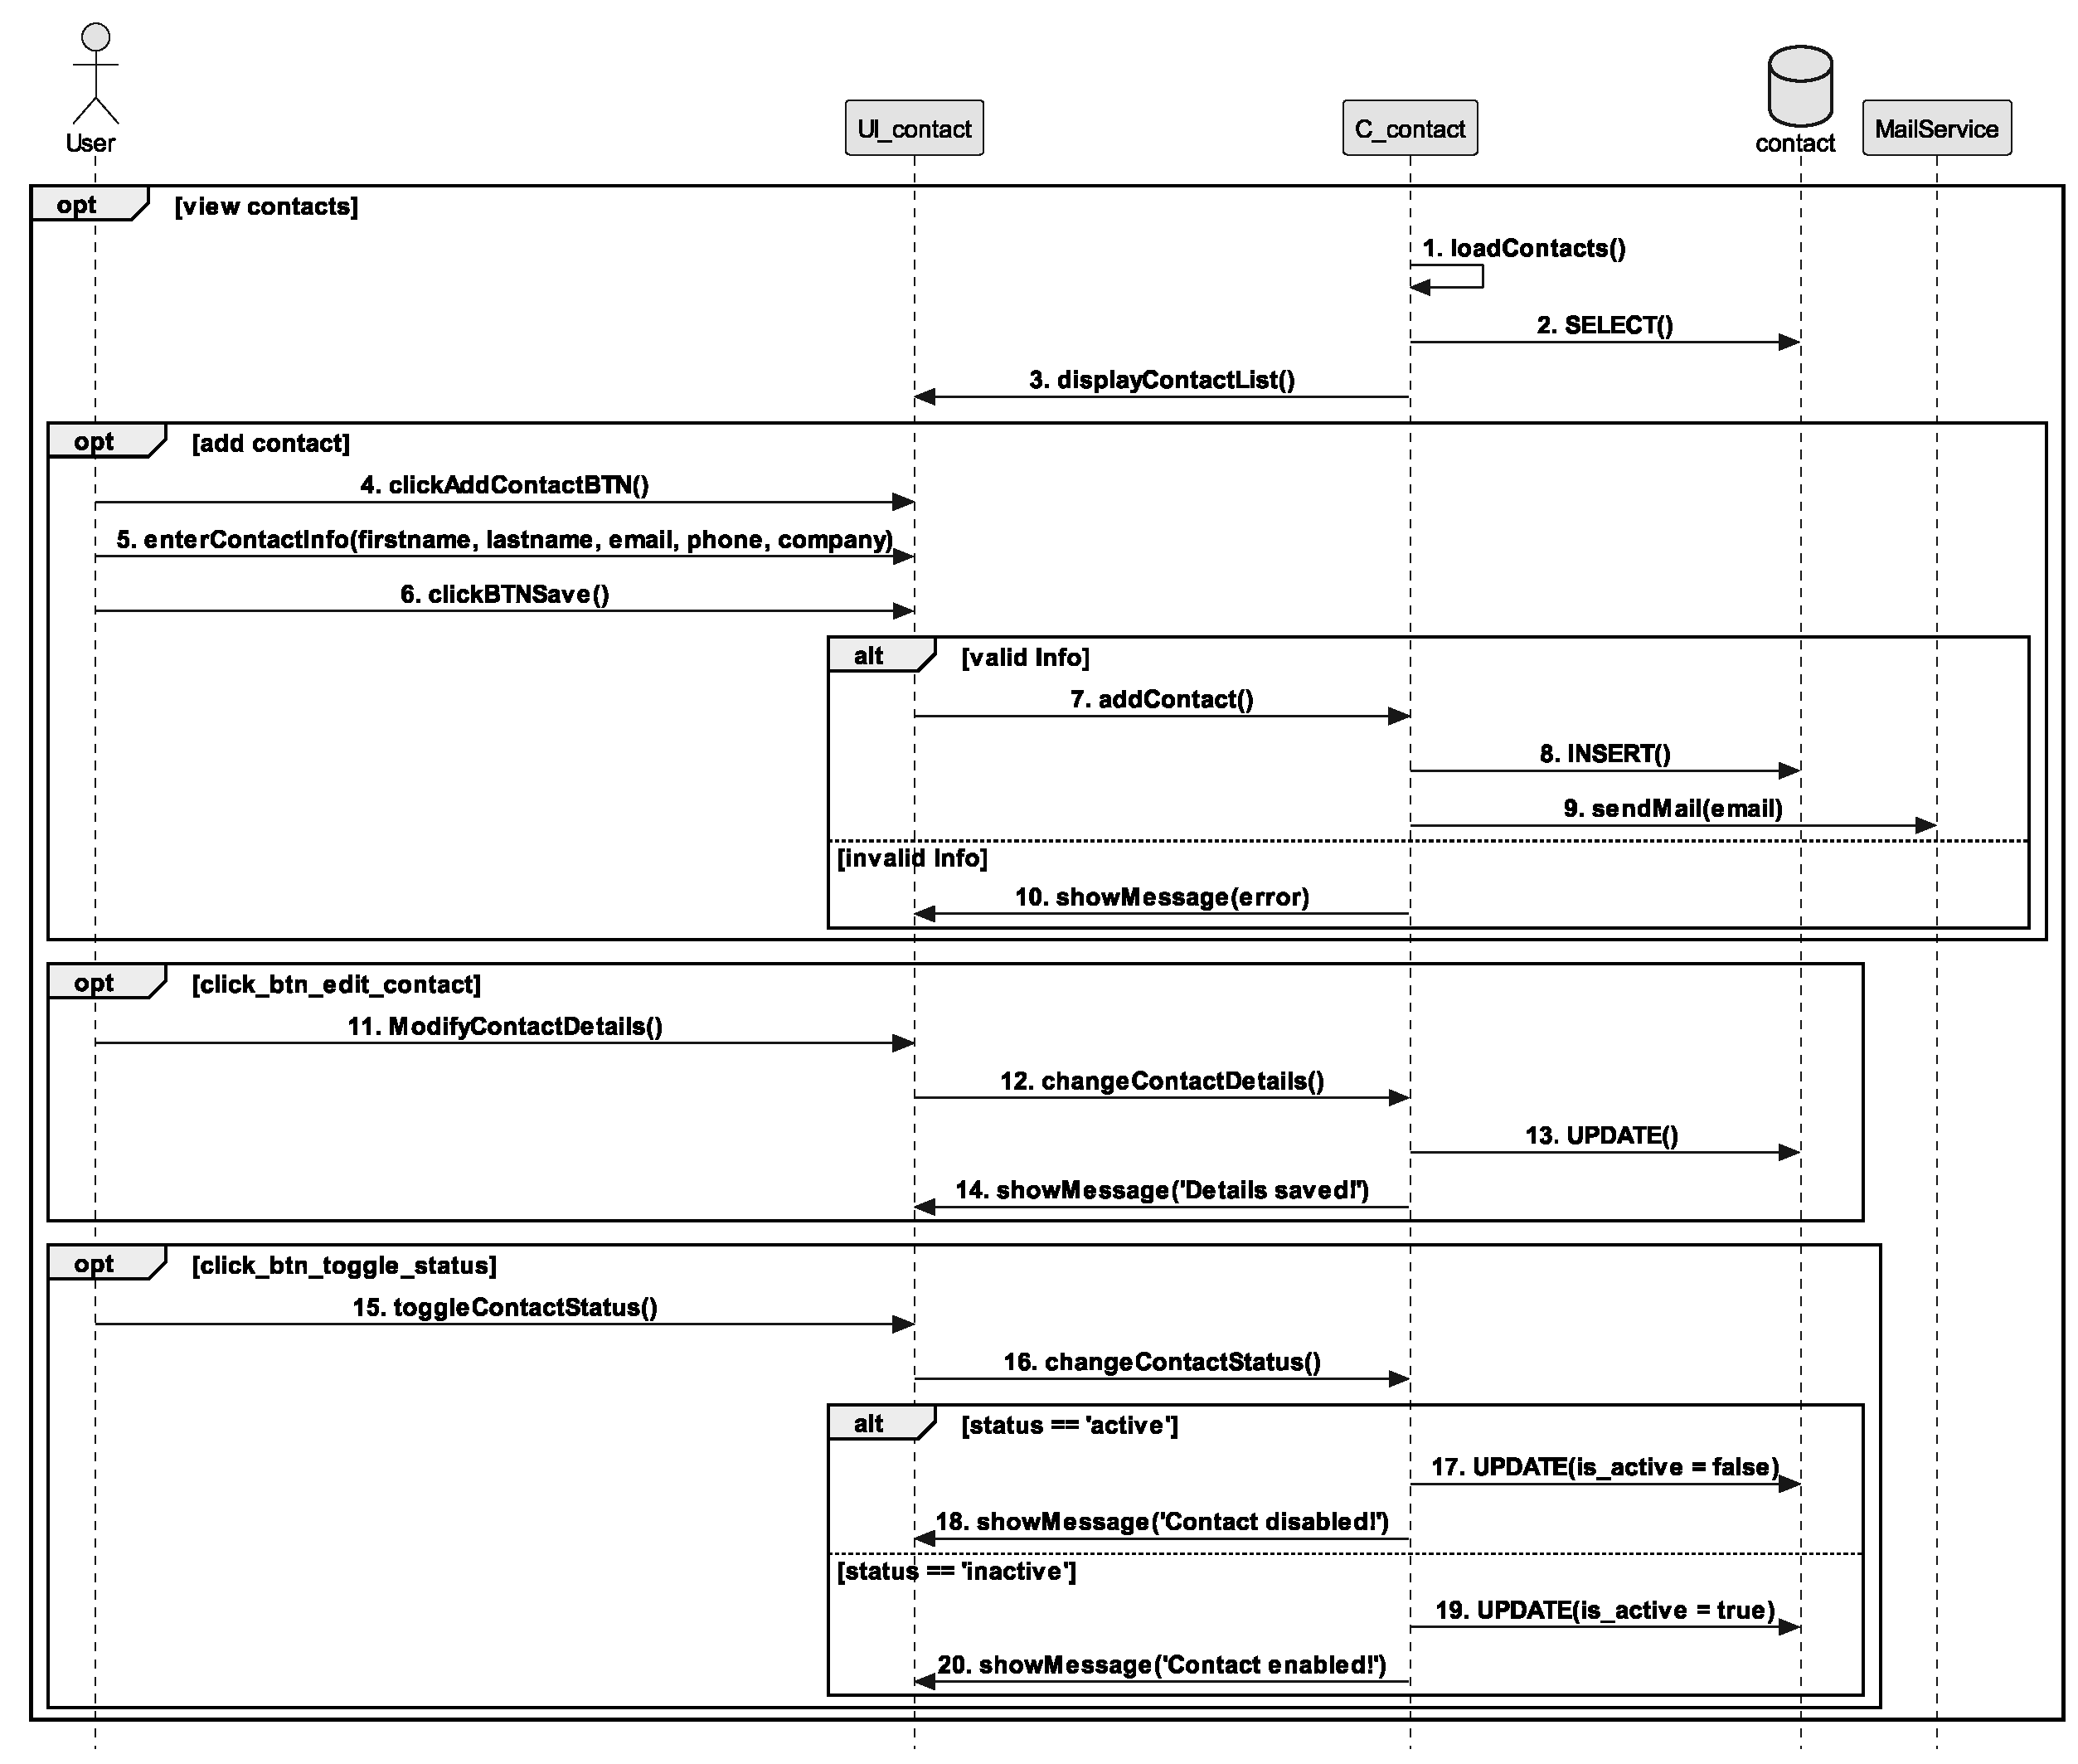
\includegraphics[width=1.2\textwidth]{images/out/diagrams/seq/manage_contacts/manage_contacts.eps}}
    \caption{Sequence Diagram -- Manage contacts}
    \label{fig:seq_manage_contacts}
\end{figure}

\newpage
\subsection{Sequence Diagram -- Use Case ``Manage companies''}
The sequence diagram below models company profile creation, editing, and directory lookup interactions:

\begin{figure}[H]
    \centering
    \makebox[\textwidth][c]{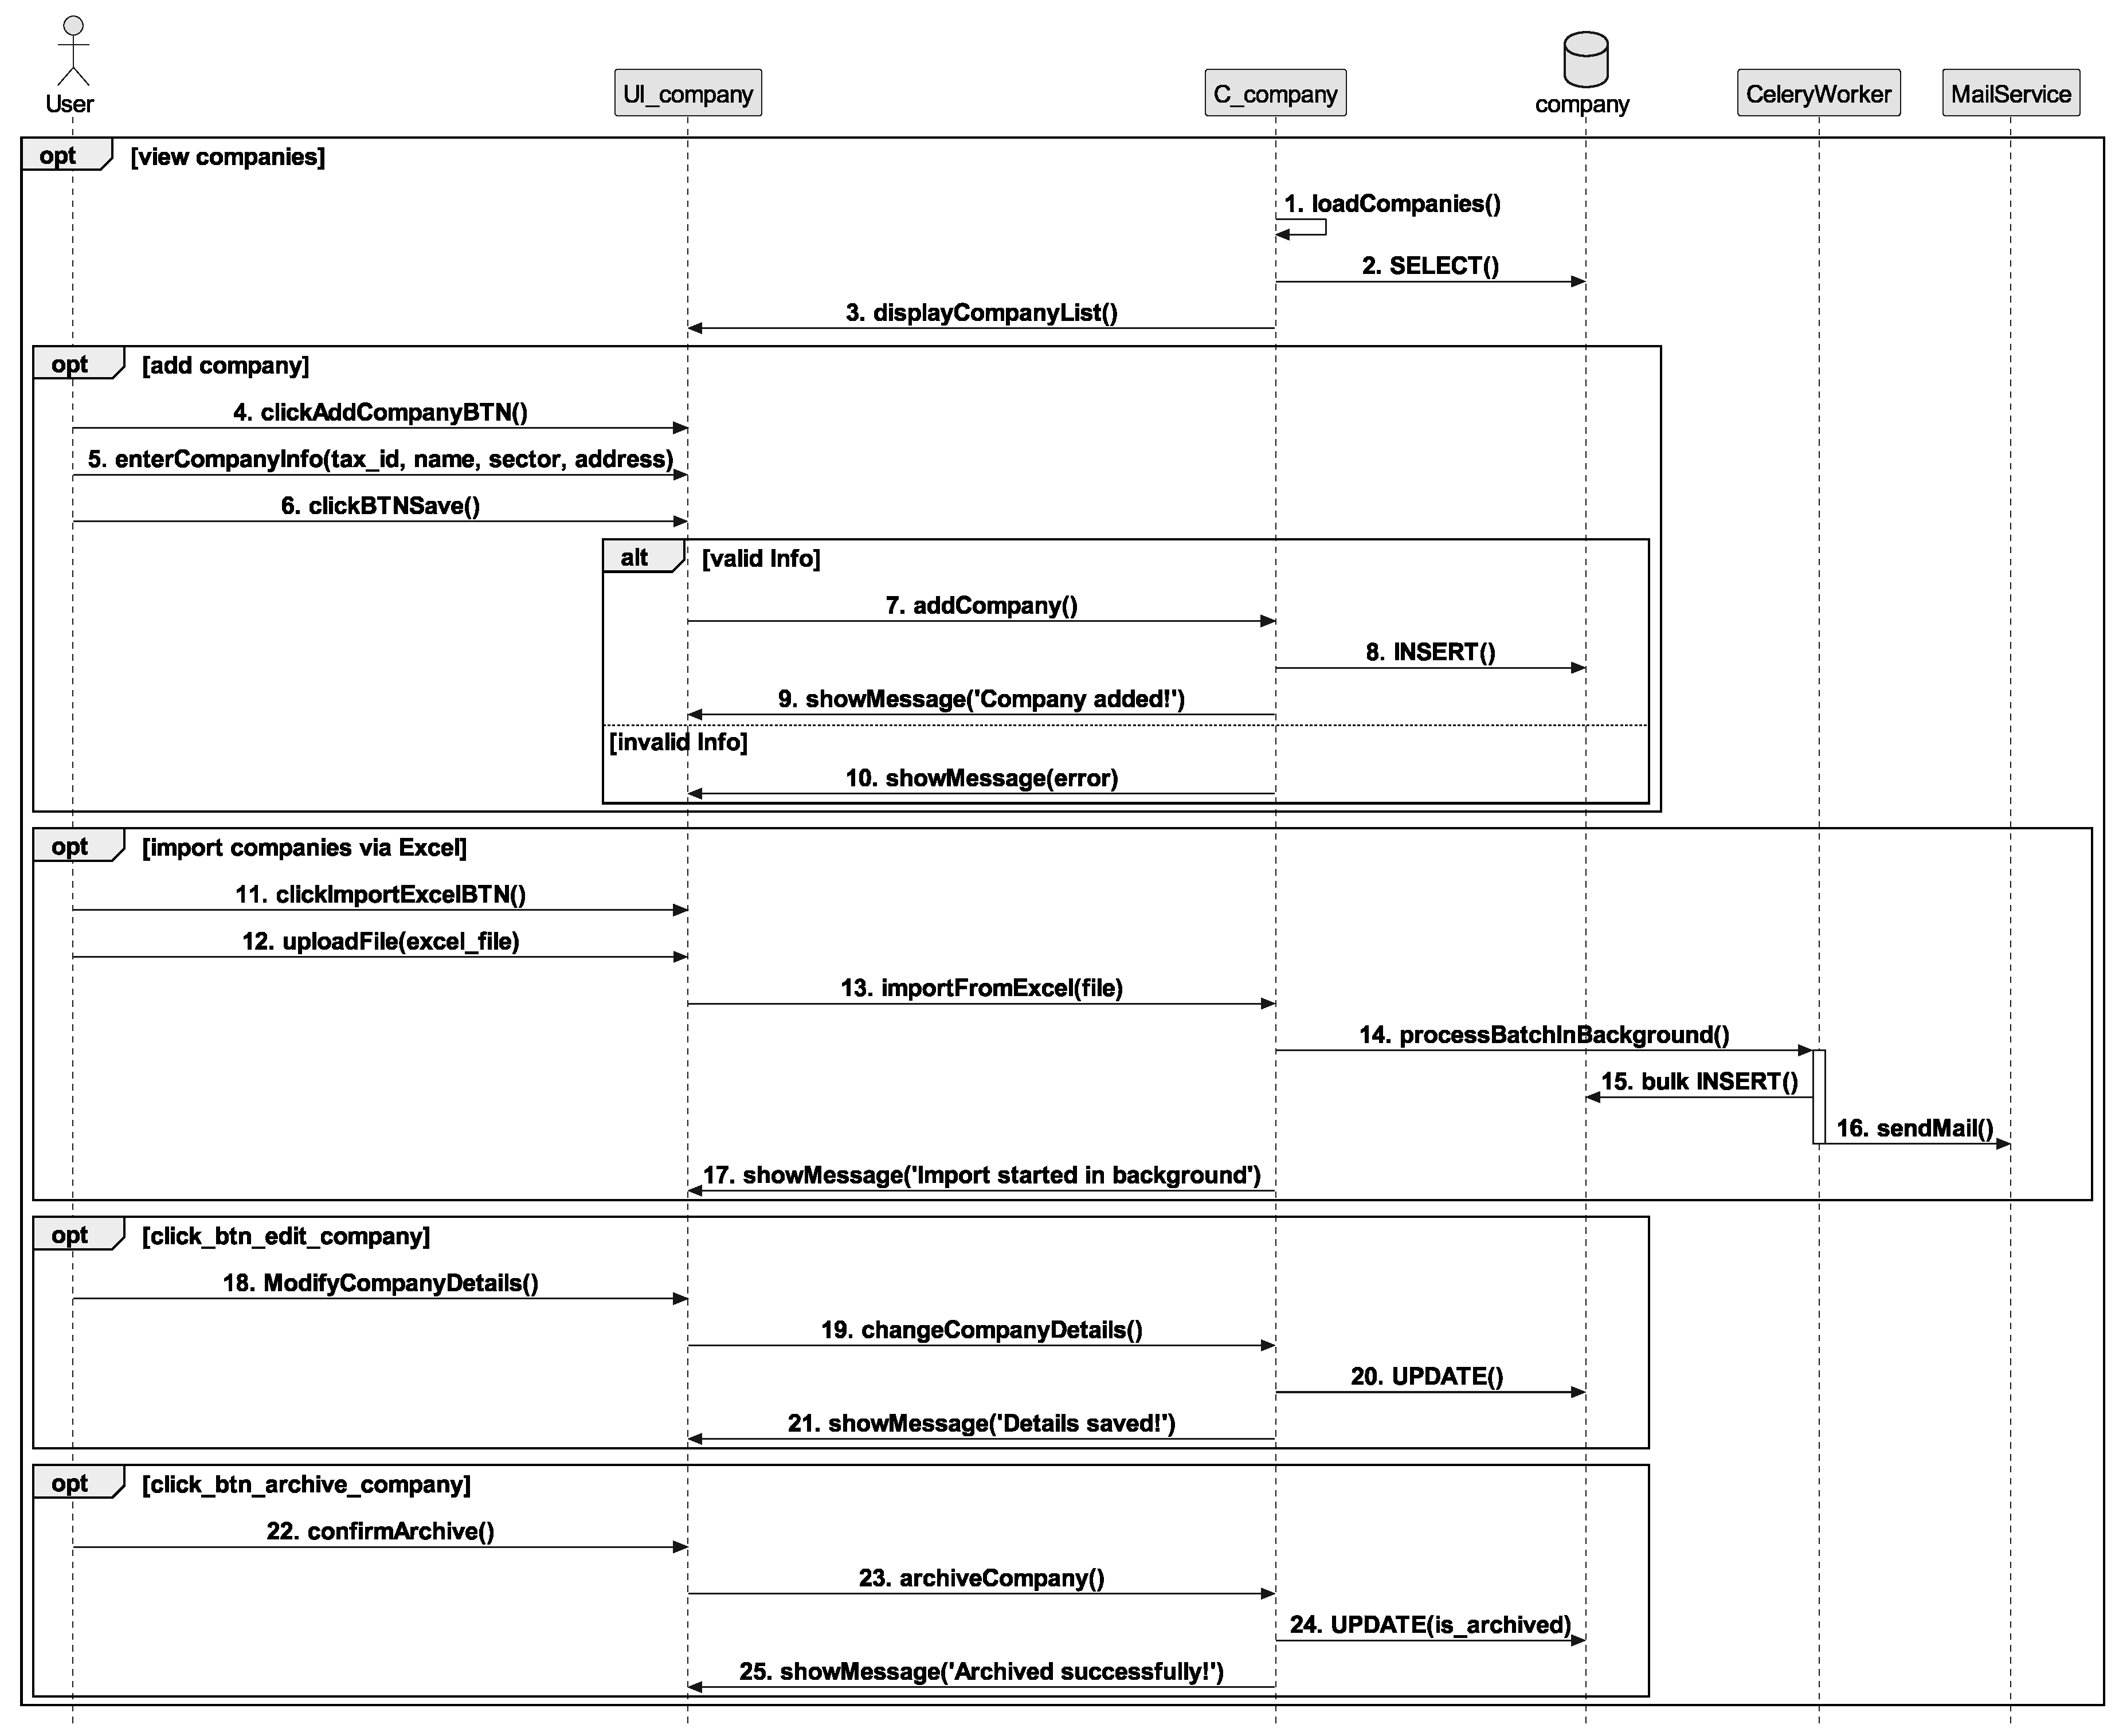
\includegraphics[width=1.2\textwidth]{images/out/diagrams/seq/manage_companies/manage_companies.eps}}
    \caption{Sequence Diagram -- Manage companies}
    \label{fig:seq_manage_companies}
\end{figure}
\newpage
\subsection{Activity and State Diagrams -- Use Case ``Manage surveys''}
Due to the complexity of the survey management process, the dynamic behavior is modeled using both an Activity Diagram and a State Machine Diagram. The activity diagram illustrates the workflow of defining a survey, configuring passages, uploading templates, and assigning targeted company samples. The state diagram models the lifecycle of a survey passage from draft to archiving.
\begin{figure}[H]
    \centering
    \makebox[\textwidth][c]{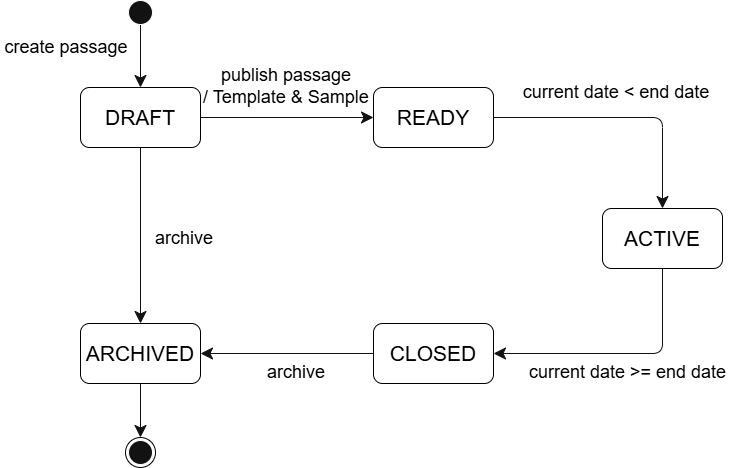
\includegraphics[width=1.0\textwidth]{images/out/diagrams/state/manage_survey/survey_etat.png}}
    \caption{State Diagram -- Manage surveys}
    \label{fig:state_manage_surveys}
\end{figure}
\begin{figure}[H]
    \centering
    \makebox[\textwidth][c]{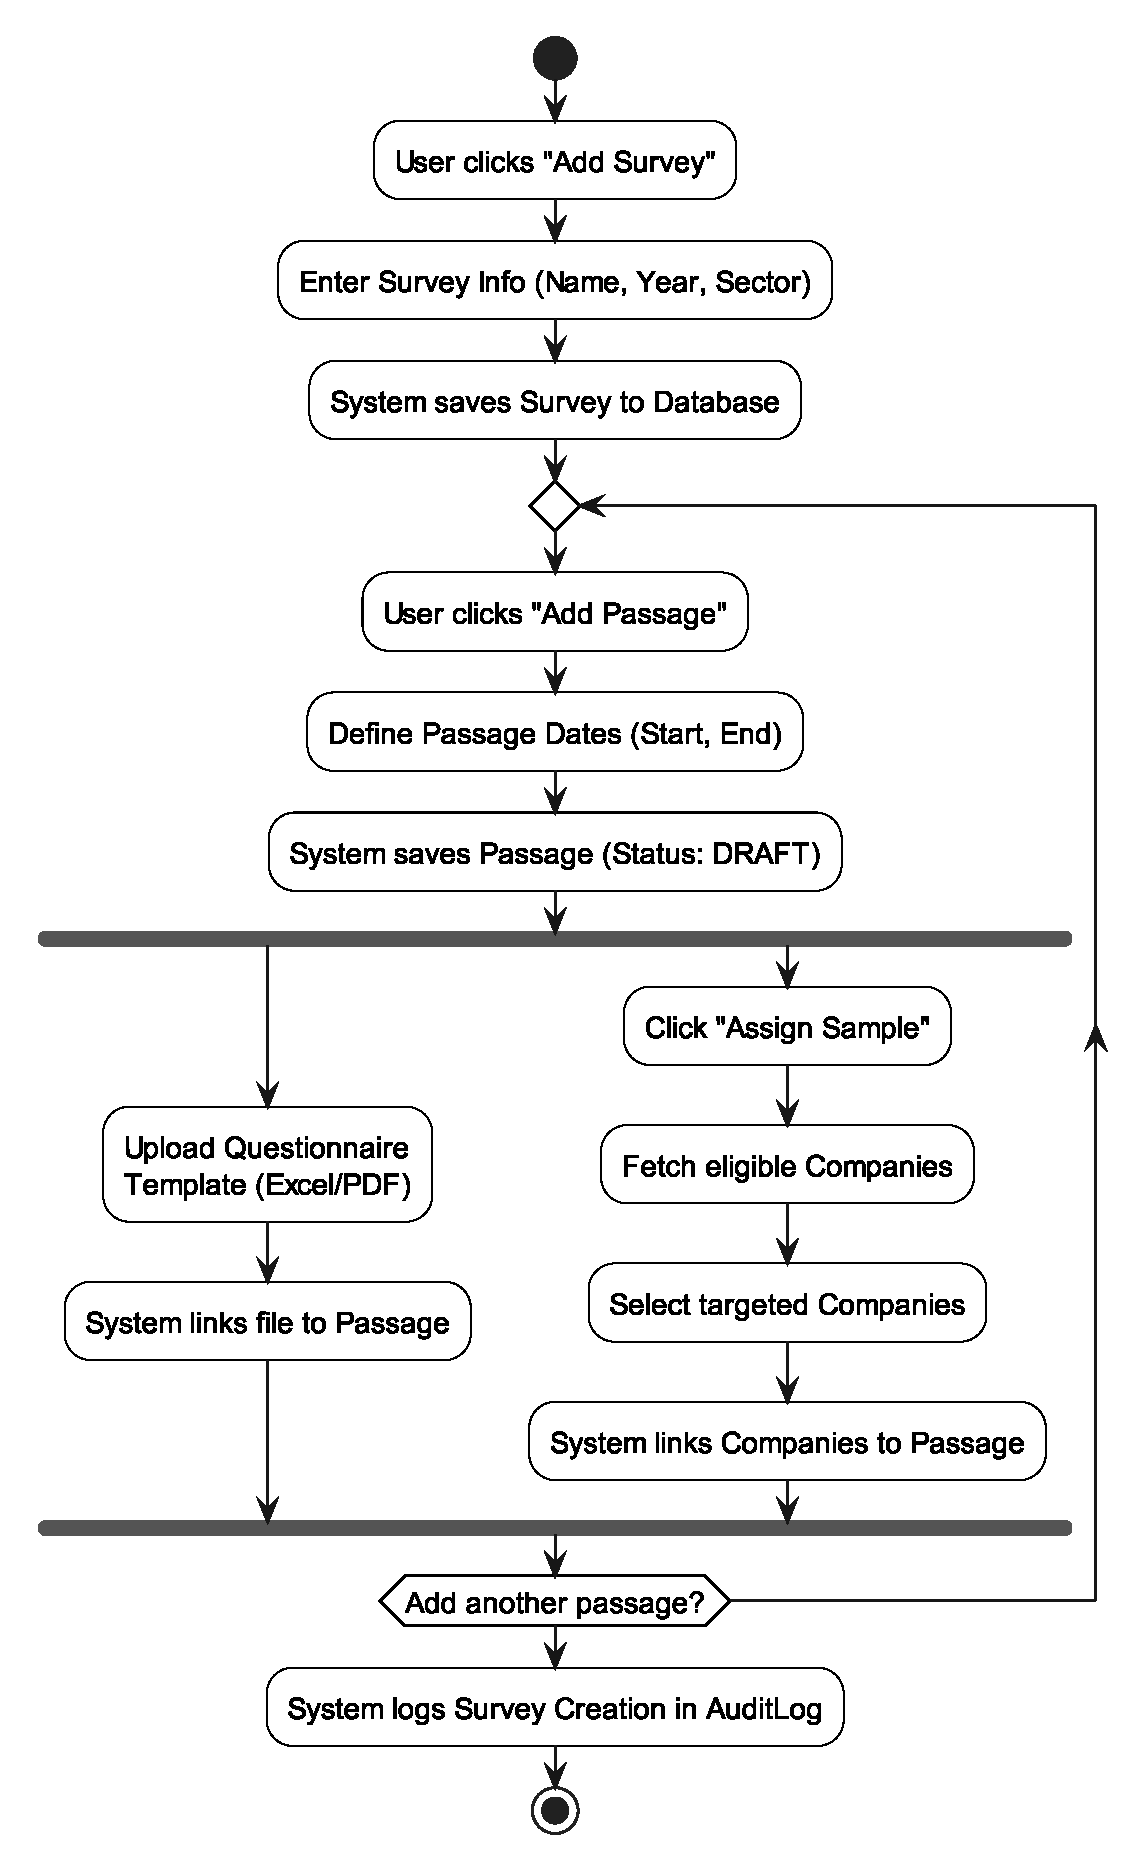
\includegraphics[width=0.8\textwidth]{images/out/diagrams/activite/manage_survey/manage_survey.eps}}
    \caption{Activity Diagram -- Manage surveys}
    \label{fig:act_manage_surveys}
\end{figure}



\newpage
\section{Sprint 0 Implementation}
This section presents the user interface implementations developed during Sprint 0, demonstrating the core authentication and administrative flows.

\subsection{Login Interface}
The authentication module provides secure access to the platform. It handles credential validation, two-factor authentication via OTP, and first-time password resets.

\begin{figure}[H]
    \centering
    \makebox[\textwidth][c]{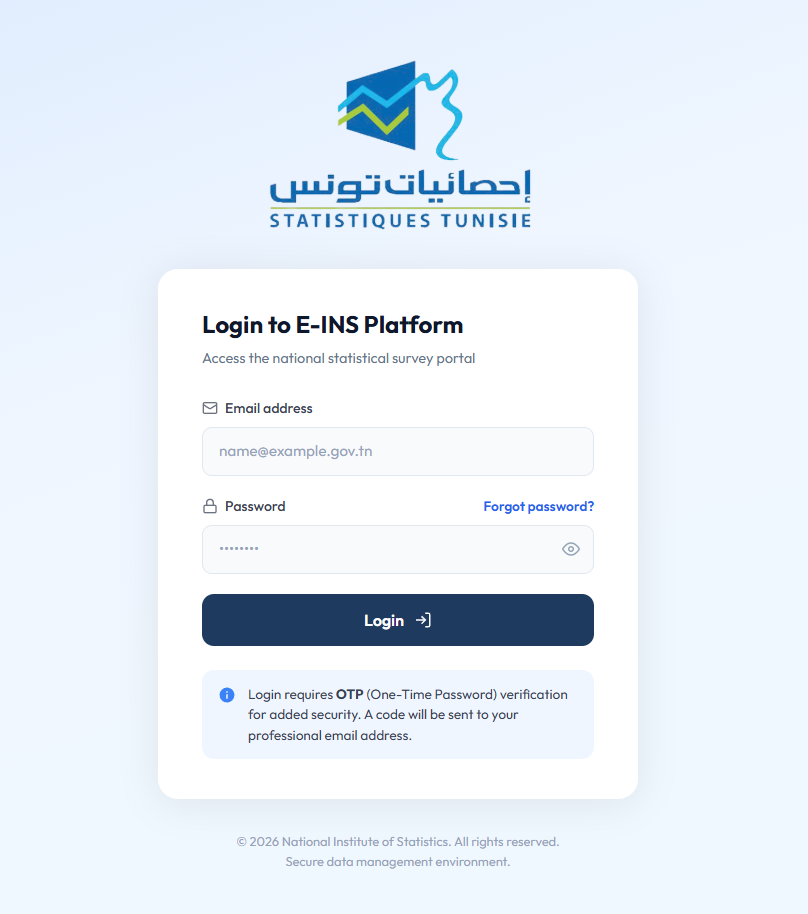
\includegraphics[width=0.9\textwidth]{images/screenshots/sprint0/login.png}}
    \caption{Login Interface}
    \label{fig:ui_login}
\end{figure}

\begin{figure}[H]
    \centering
    \makebox[\textwidth][c]{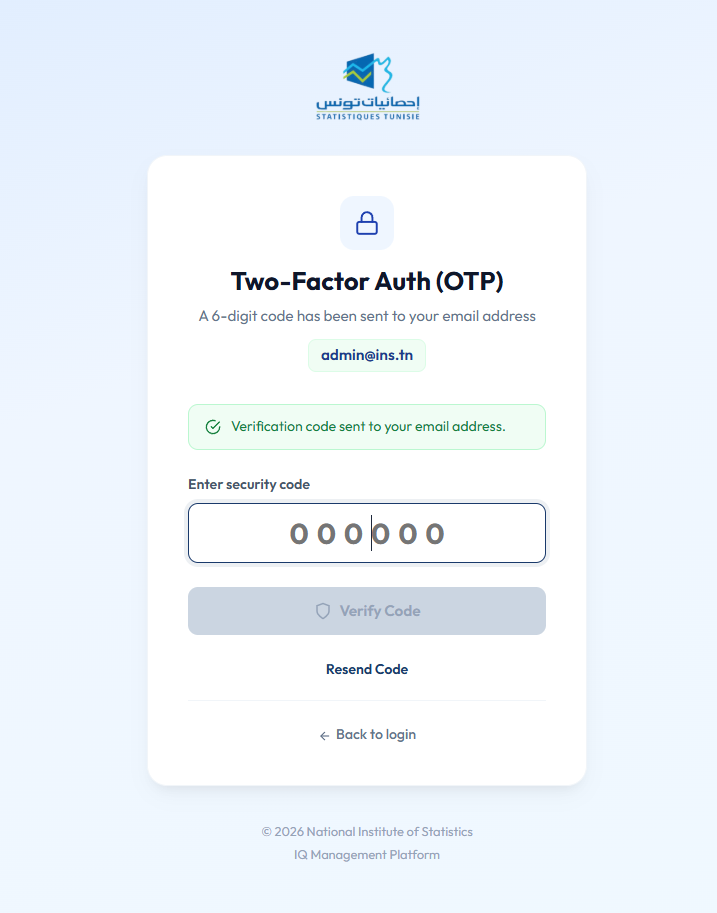
\includegraphics[width=0.9\textwidth]{images/screenshots/sprint0/OTP.png}}
    \caption{OTP Verification Interface}
    \label{fig:ui_otp}
\end{figure}

\begin{figure}[H]
    \centering
    \makebox[\textwidth][c]{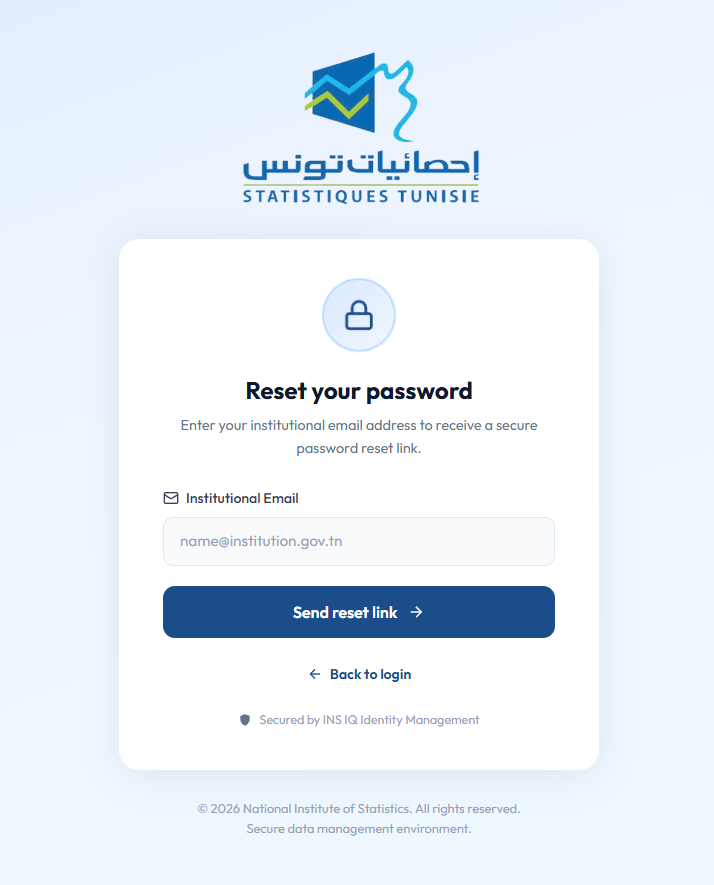
\includegraphics[width=0.9\textwidth]{images/screenshots/sprint0/resetpassword.png}}
    \caption{Reset Password Interface}
    \label{fig:ui_reset_password}
\end{figure}

\subsection{Security Architecture}
The platform enforces configurable authentication security parameters at the system-settings level: OTP codes expire after 5 minutes by default, accounts lock after 3 failed sign-in attempts, lockouts last 24 hours, and a 1-hour password-only bypass window is granted after manual administrator unlock. Authentication tokens are issued as JSON Web Tokens (JWT) signed with the HS256 algorithm and a 24-hour expiration duration, configured via Pydantic Settings loaded from environment variables (\texttt{.env}). To ensure immediate access revocation upon logout, each token includes a unique \texttt{jti} claim that is blacklisted in Redis until expiration. On the client side, the Angular application manages user session tokens via \texttt{localStorage} and injects them automatically into outgoing HTTP headers through a custom HTTP interceptor. API endpoints enforce access control via FastAPI's \texttt{Depends(get\_current\_user)} dependency guard. Listing \ref{lst:jwt_security} illustrates the backend token creation implementation incorporating the \texttt{jti} blacklist mechanism.

\begin{lstlisting}[language=Python, caption={JWT Token Generation with Blacklist Support (\texttt{app/core/security.py})}, label={lst:jwt_security}]
def create_access_token(
    data: dict, 
    expires_delta: Optional[datetime.timedelta] = None
) -> str:
    to_encode = data.copy()
    ttl = expires_delta or datetime.timedelta(
        minutes=settings.ACCESS_TOKEN_EXPIRE_MINUTES
    )
    expire = datetime.datetime.now() + ttl
    # Unique JWT ID (jti) for logout blacklisting
    to_encode.update({
        "exp": expire,
        "jti": secrets.token_hex(16),
    })
    return jwt.encode(
        to_encode, 
        settings.SECRET_KEY, 
        algorithm=settings.ALGORITHM
    )
\end{lstlisting}

\newpage
\subsection{Manage admins Interface}
The admin management interface allows the System Administrator to view, filter, create, and update administrative accounts across system roles.

\begin{figure}[H]
    \centering
    \makebox[\textwidth][c]{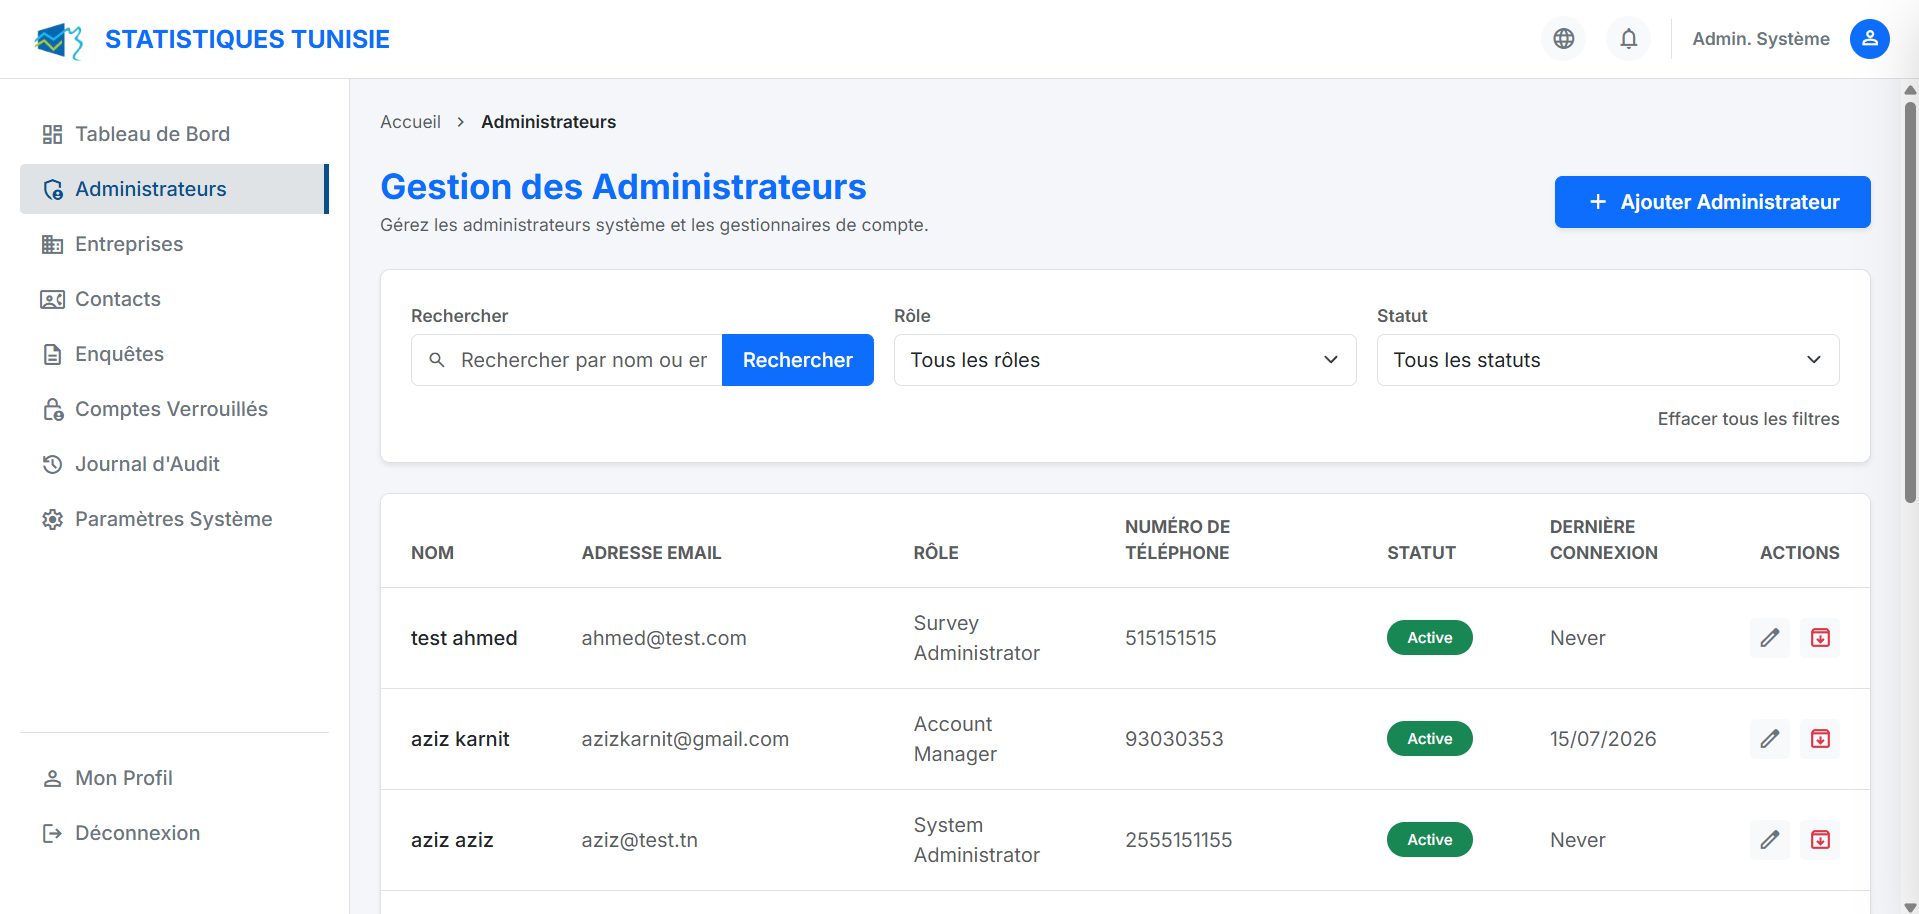
\includegraphics[width=1.1\textwidth]{images/screenshots/sprint0/admin_page.png}}
    \caption{Admin Directory Interface}
    \label{fig:ui_admin_page}
\end{figure}

\begin{figure}[H]
    \centering
    \makebox[\textwidth][c]{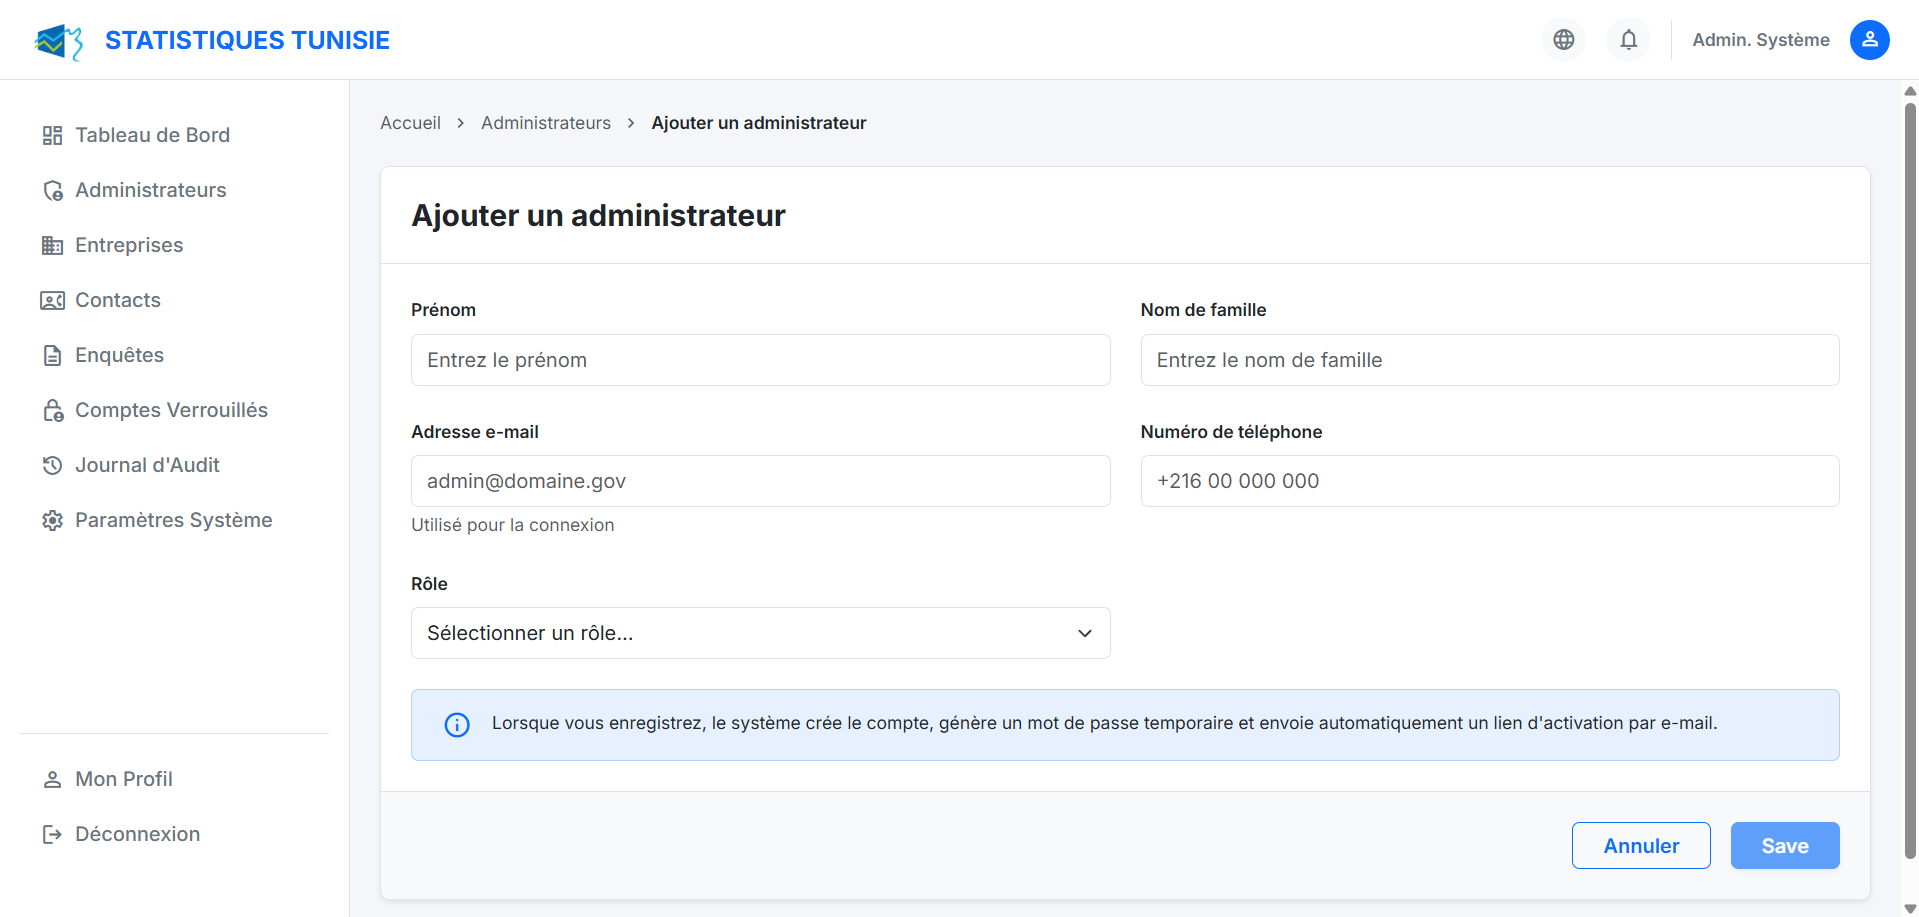
\includegraphics[width=1.1\textwidth]{images/screenshots/sprint0/add_admin.png}}
    \caption{Add Admin Form}
    \label{fig:ui_add_admin}
\end{figure}

\begin{figure}[H]
    \centering
    \makebox[\textwidth][c]{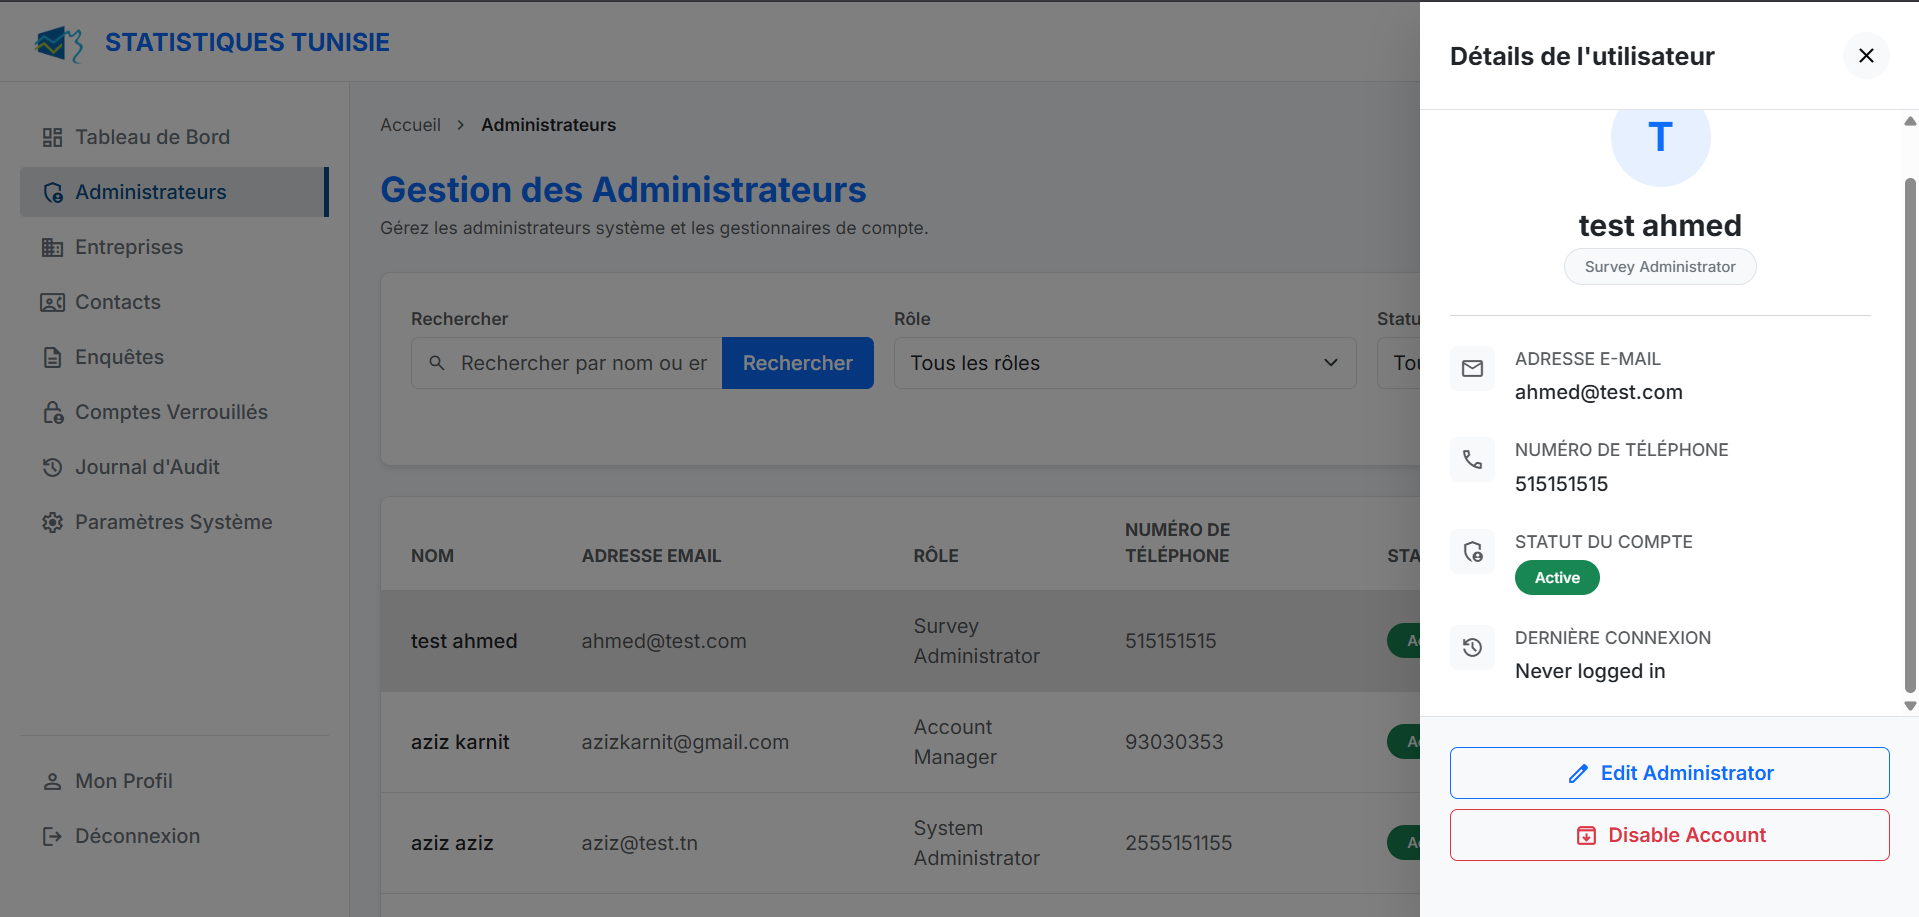
\includegraphics[width=1.1\textwidth]{images/screenshots/sprint0/edit_archive_admin.png}}
    \caption{Edit and Disable Admin Actions}
    \label{fig:ui_edit_admin}
\end{figure}

\subsection{Manage contacts Interface}
The contact directory interface enables administrators and account managers to maintain company representative profiles and link contacts to surveyed enterprises.

\begin{figure}[H]
    \centering
    \makebox[\textwidth][c]{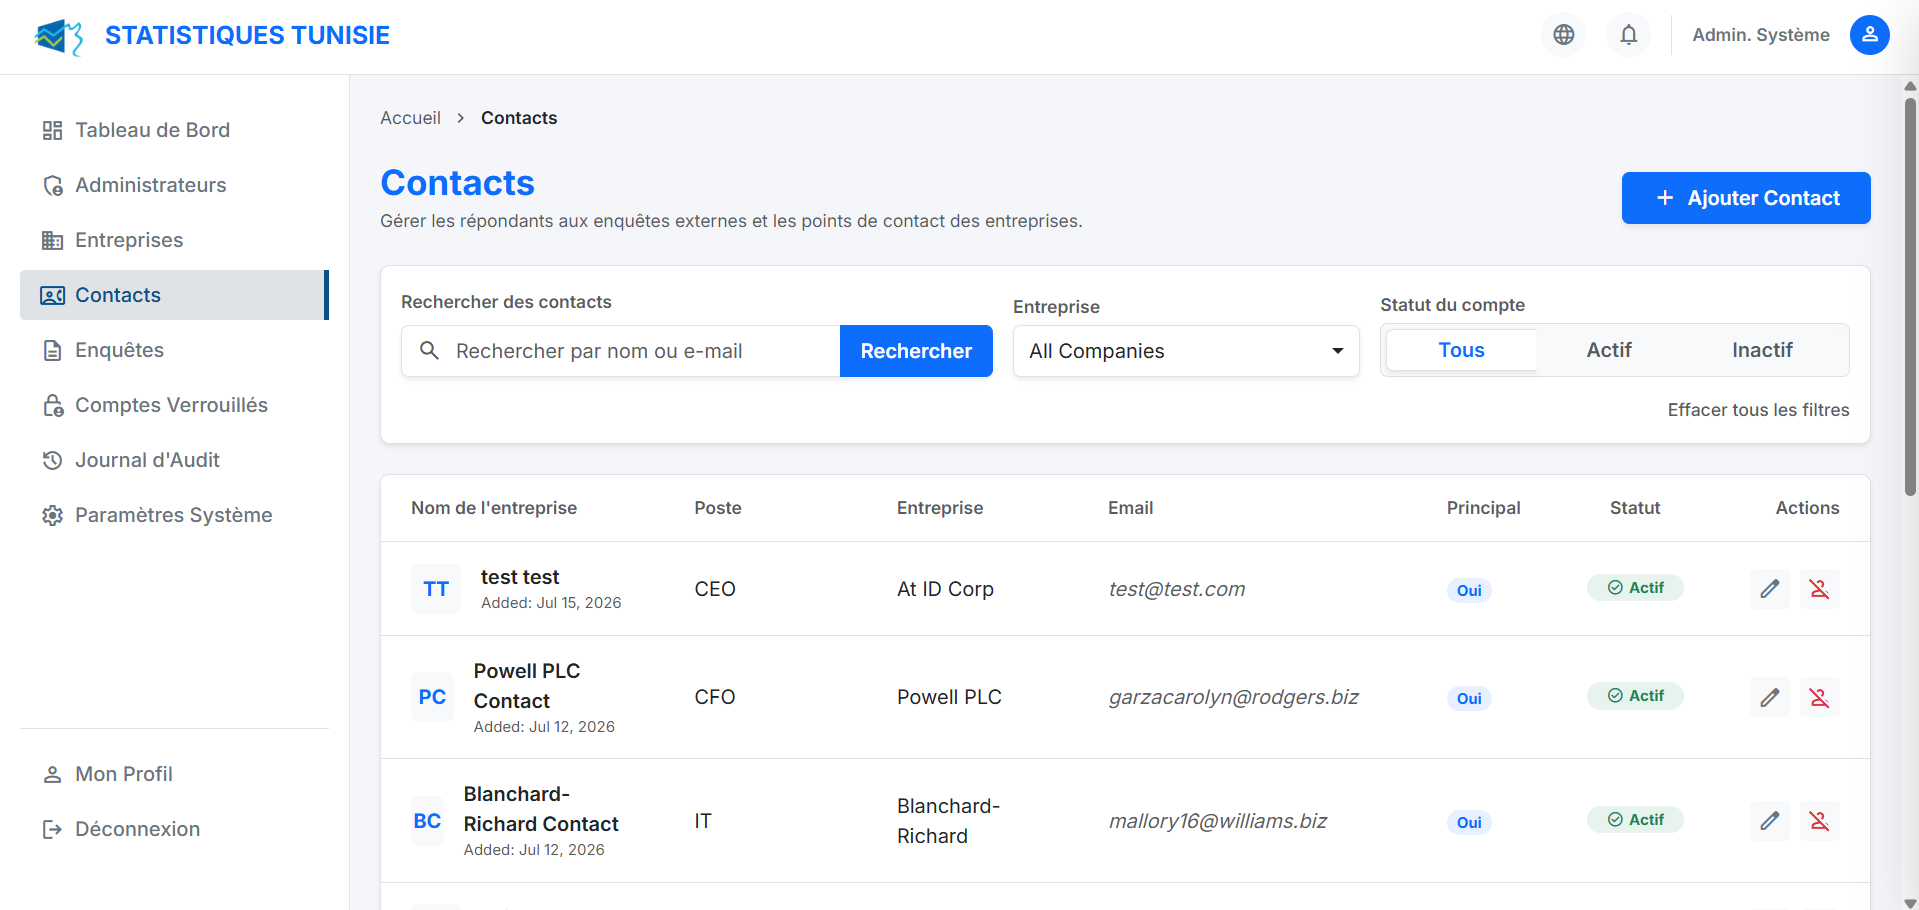
\includegraphics[width=1.1\textwidth]{images/screenshots/sprint0/contact_page.png}}
    \caption{Contact Directory Interface}
    \label{fig:ui_contact_page}
\end{figure}

\begin{figure}[H]
    \centering
    \makebox[\textwidth][c]{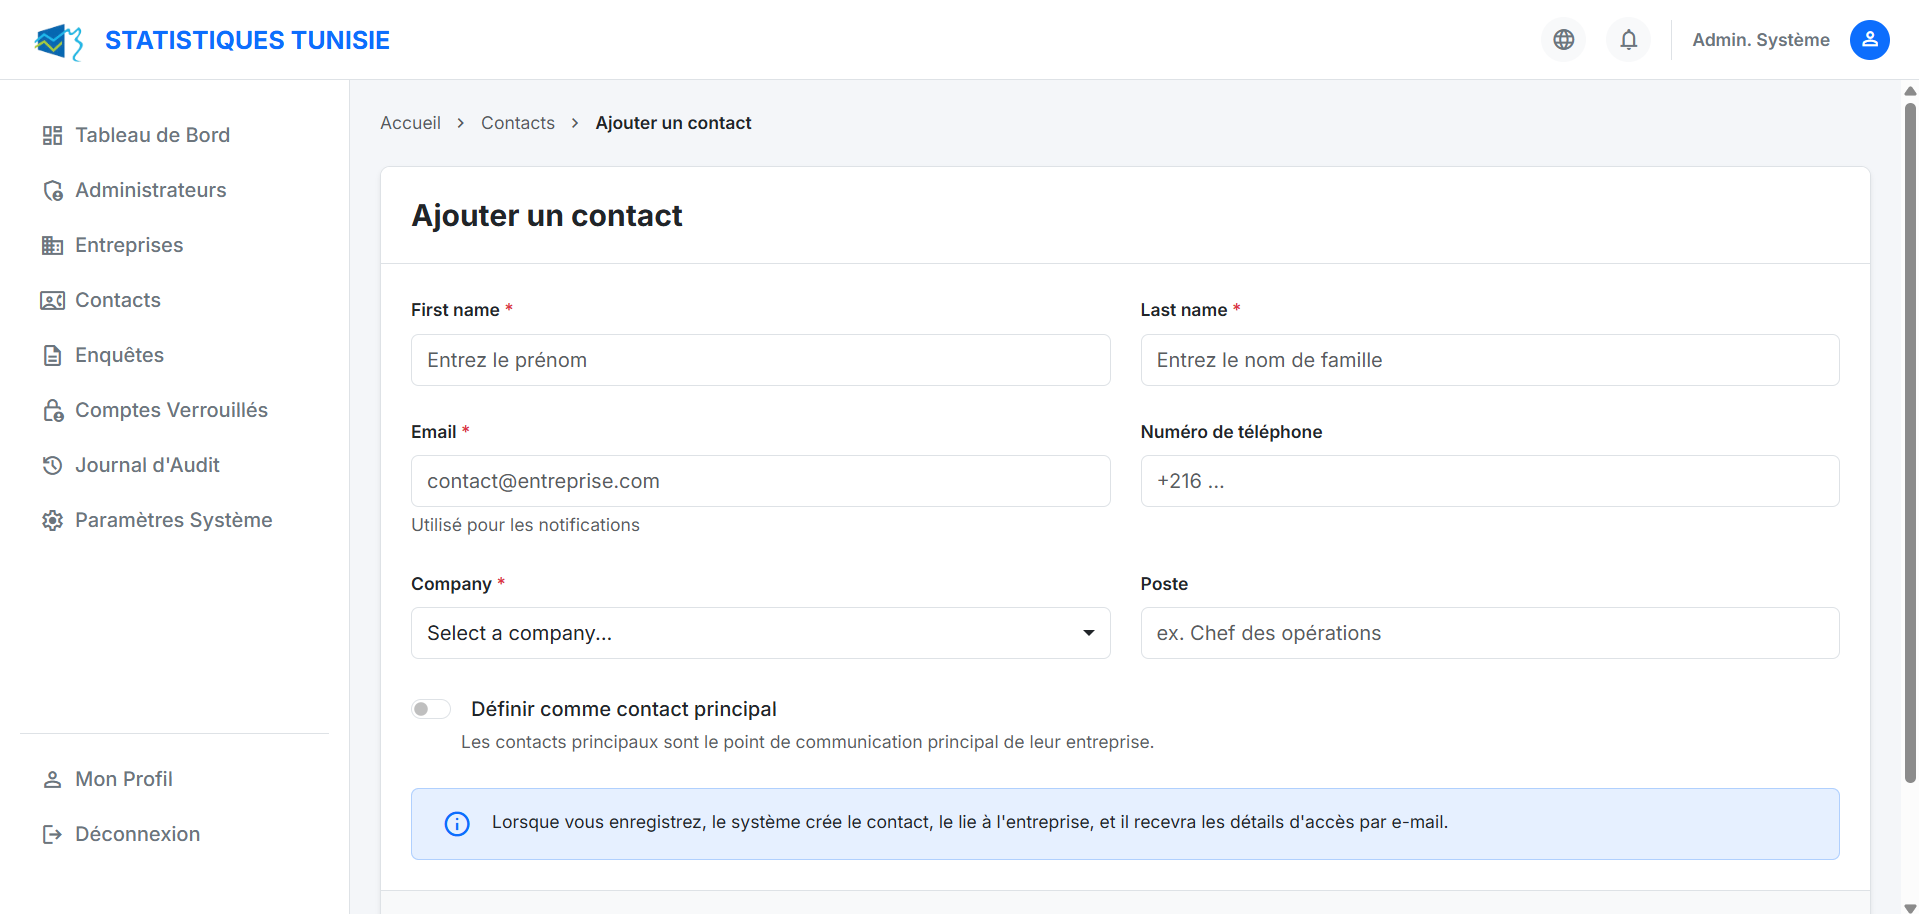
\includegraphics[width=1.1\textwidth]{images/screenshots/sprint0/add_contact.png}}
    \caption{Add Contact Form}
    \label{fig:ui_add_contact}
\end{figure}

\subsection{Manage companies Interface}
The company registry interface provides centralized administration for company master data. It supports both manual entry and asynchronous bulk Excel imports.

\begin{figure}[H]
    \centering
    \makebox[\textwidth][c]{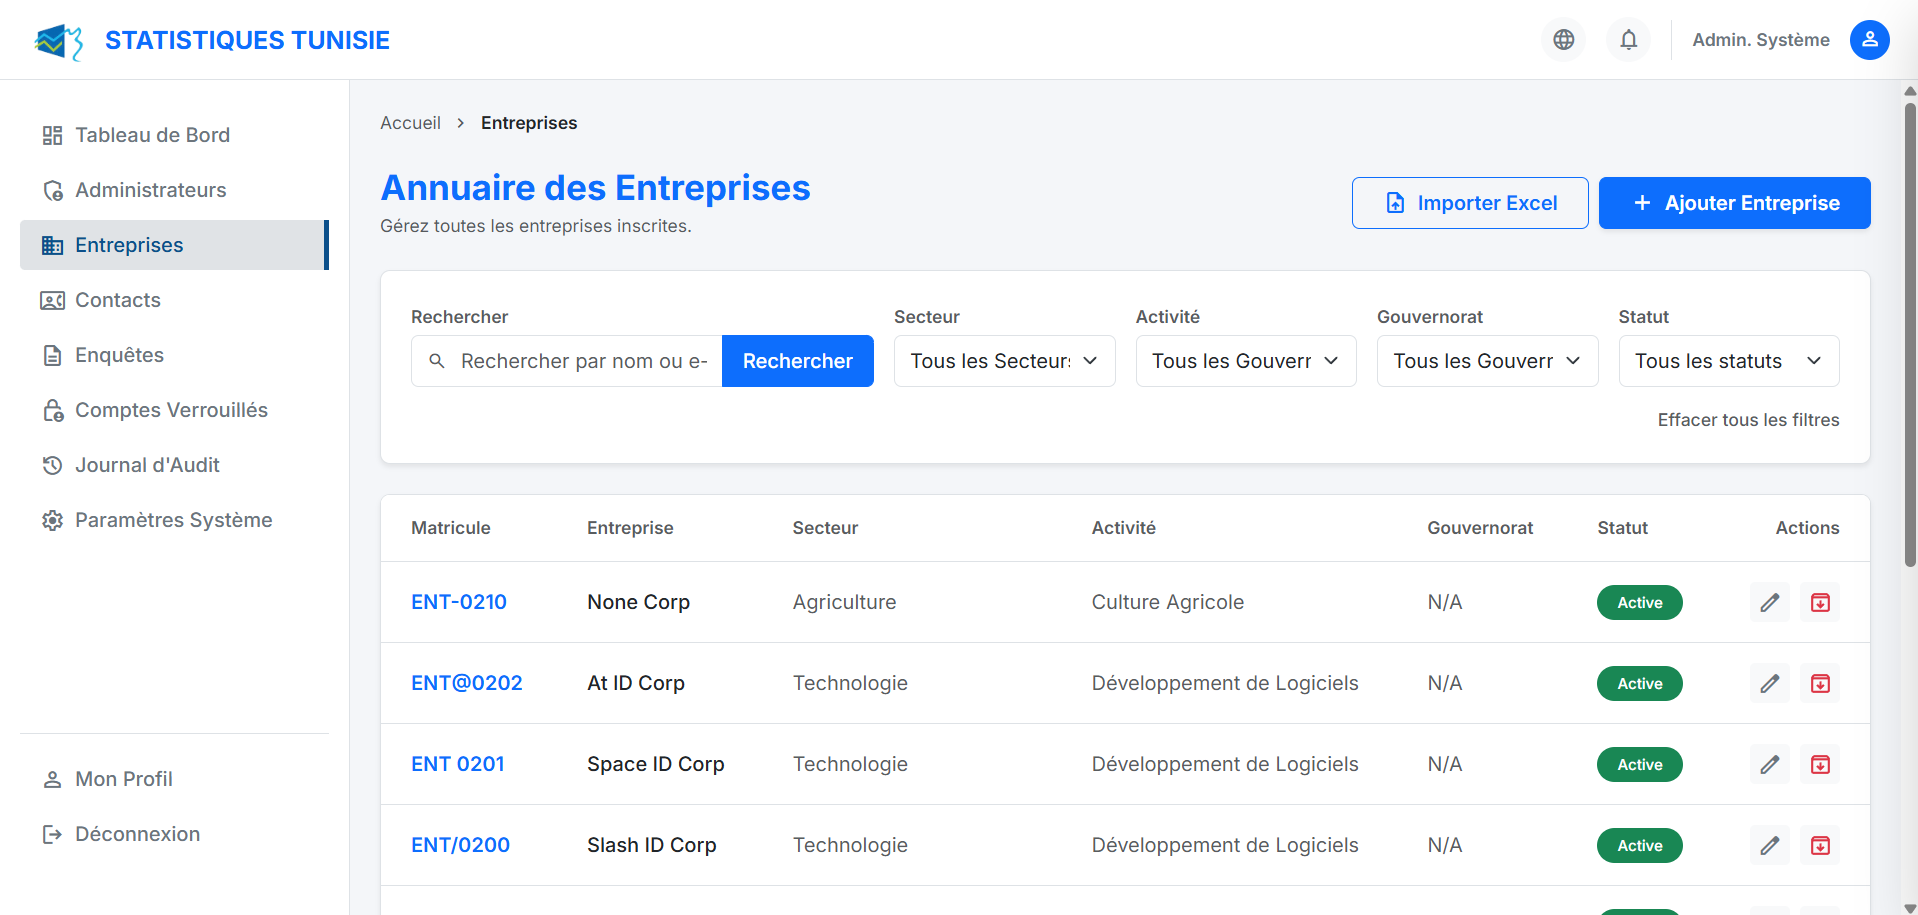
\includegraphics[width=1.1\textwidth]{images/screenshots/sprint0/company_page.png}}
    \caption{Company Directory Interface}
    \label{fig:ui_company_page}
\end{figure}

\begin{figure}[H]
    \centering
    \makebox[\textwidth][c]{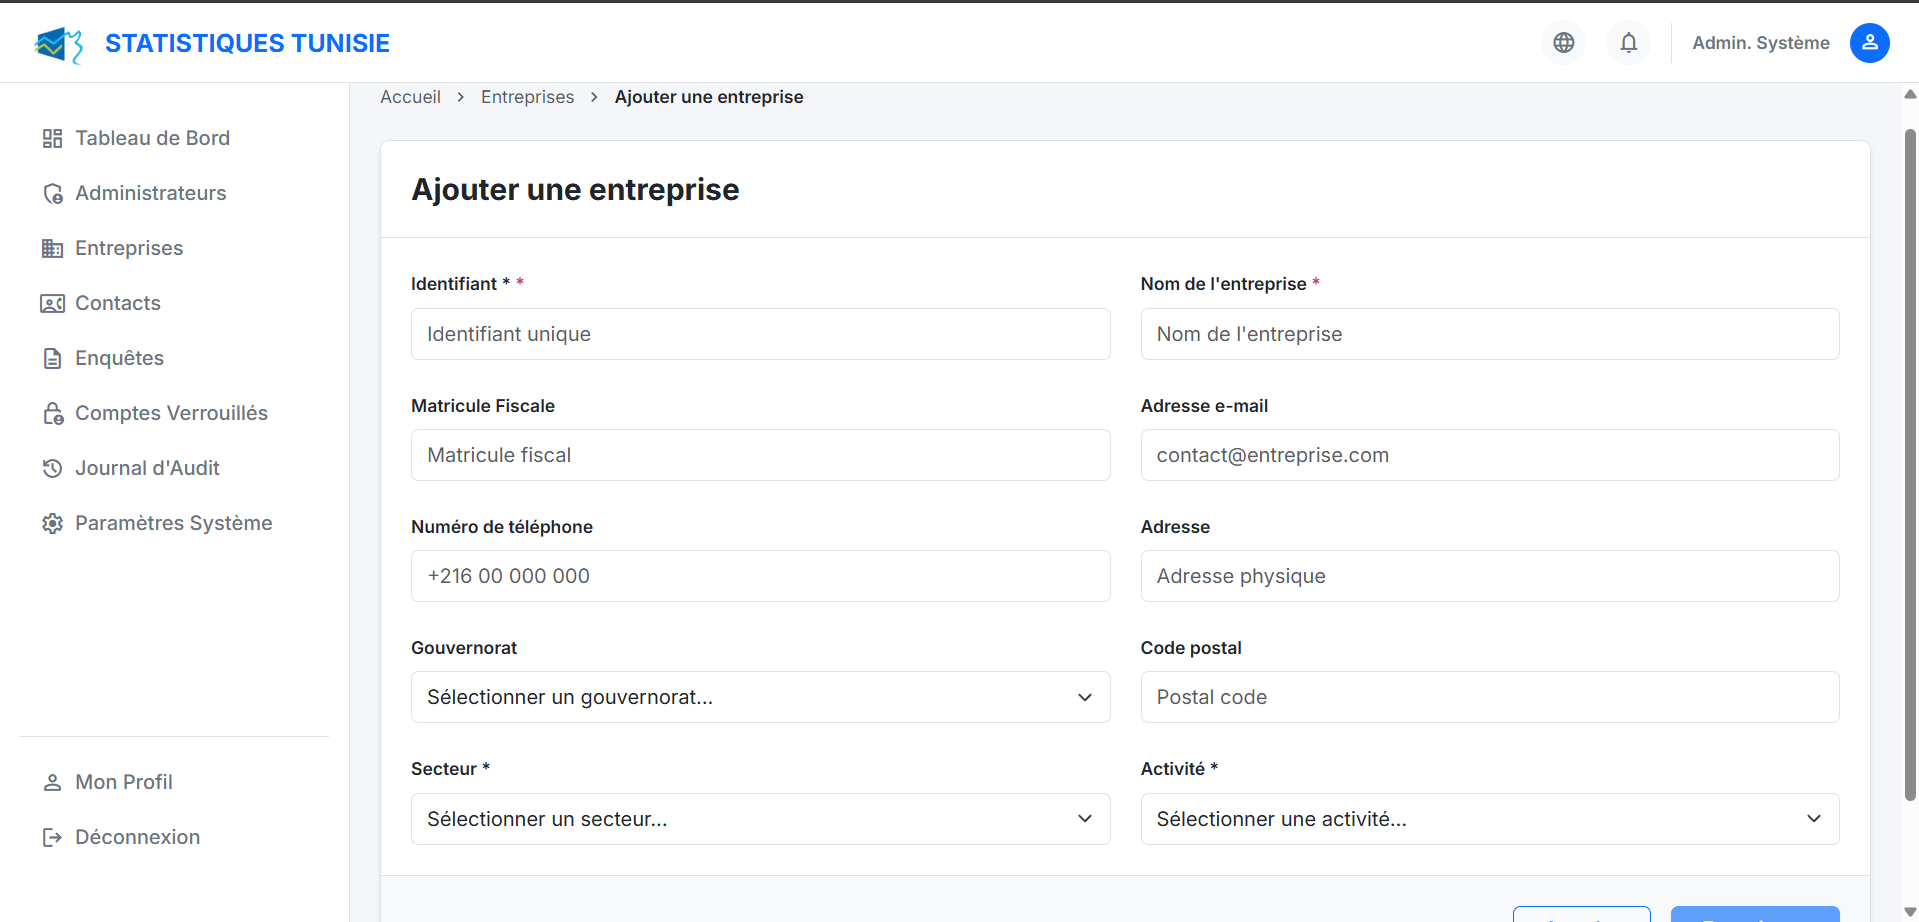
\includegraphics[width=1.1\textwidth]{images/screenshots/sprint0/add_company.png}}
    \caption{Add Company Form}
    \label{fig:ui_add_company}
\end{figure}

\begin{figure}[H]
    \centering
    \makebox[\textwidth][c]{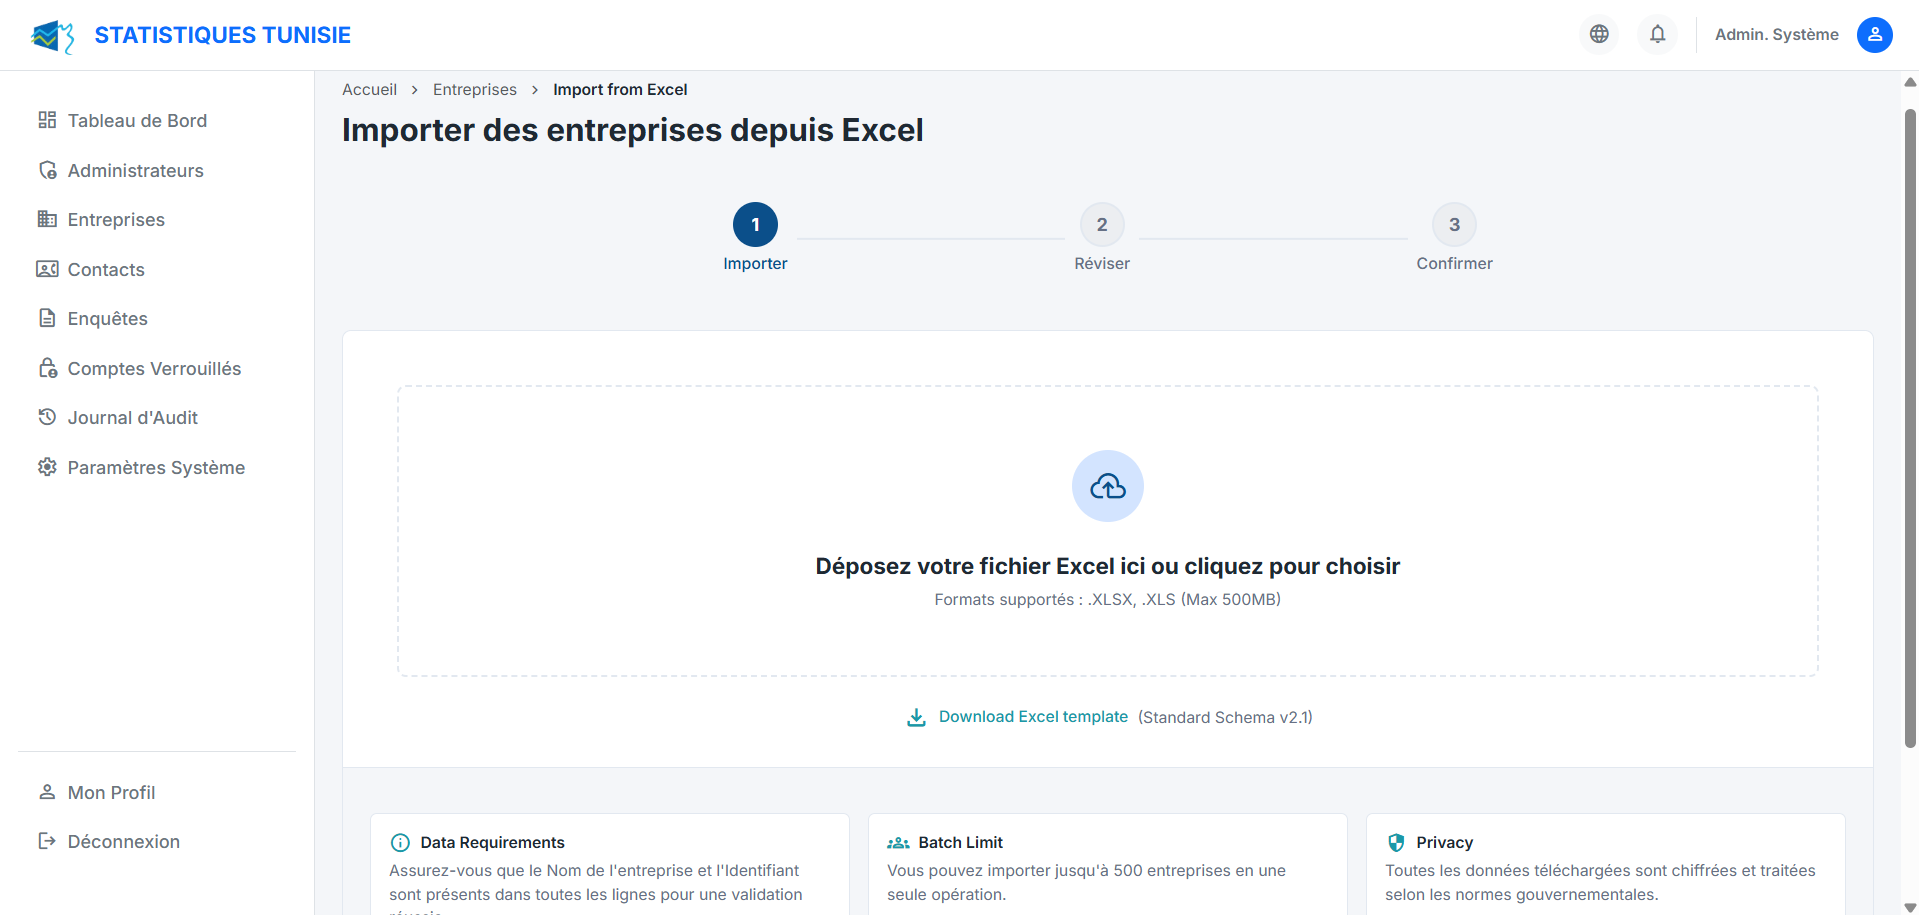
\includegraphics[width=1.1\textwidth]{images/screenshots/sprint0/batch_import_companies_first_page.png}}
    \caption{Batch Import - Upload File}
    \label{fig:ui_batch_upload}
\end{figure}

\begin{figure}[H]
    \centering
    \makebox[\textwidth][c]{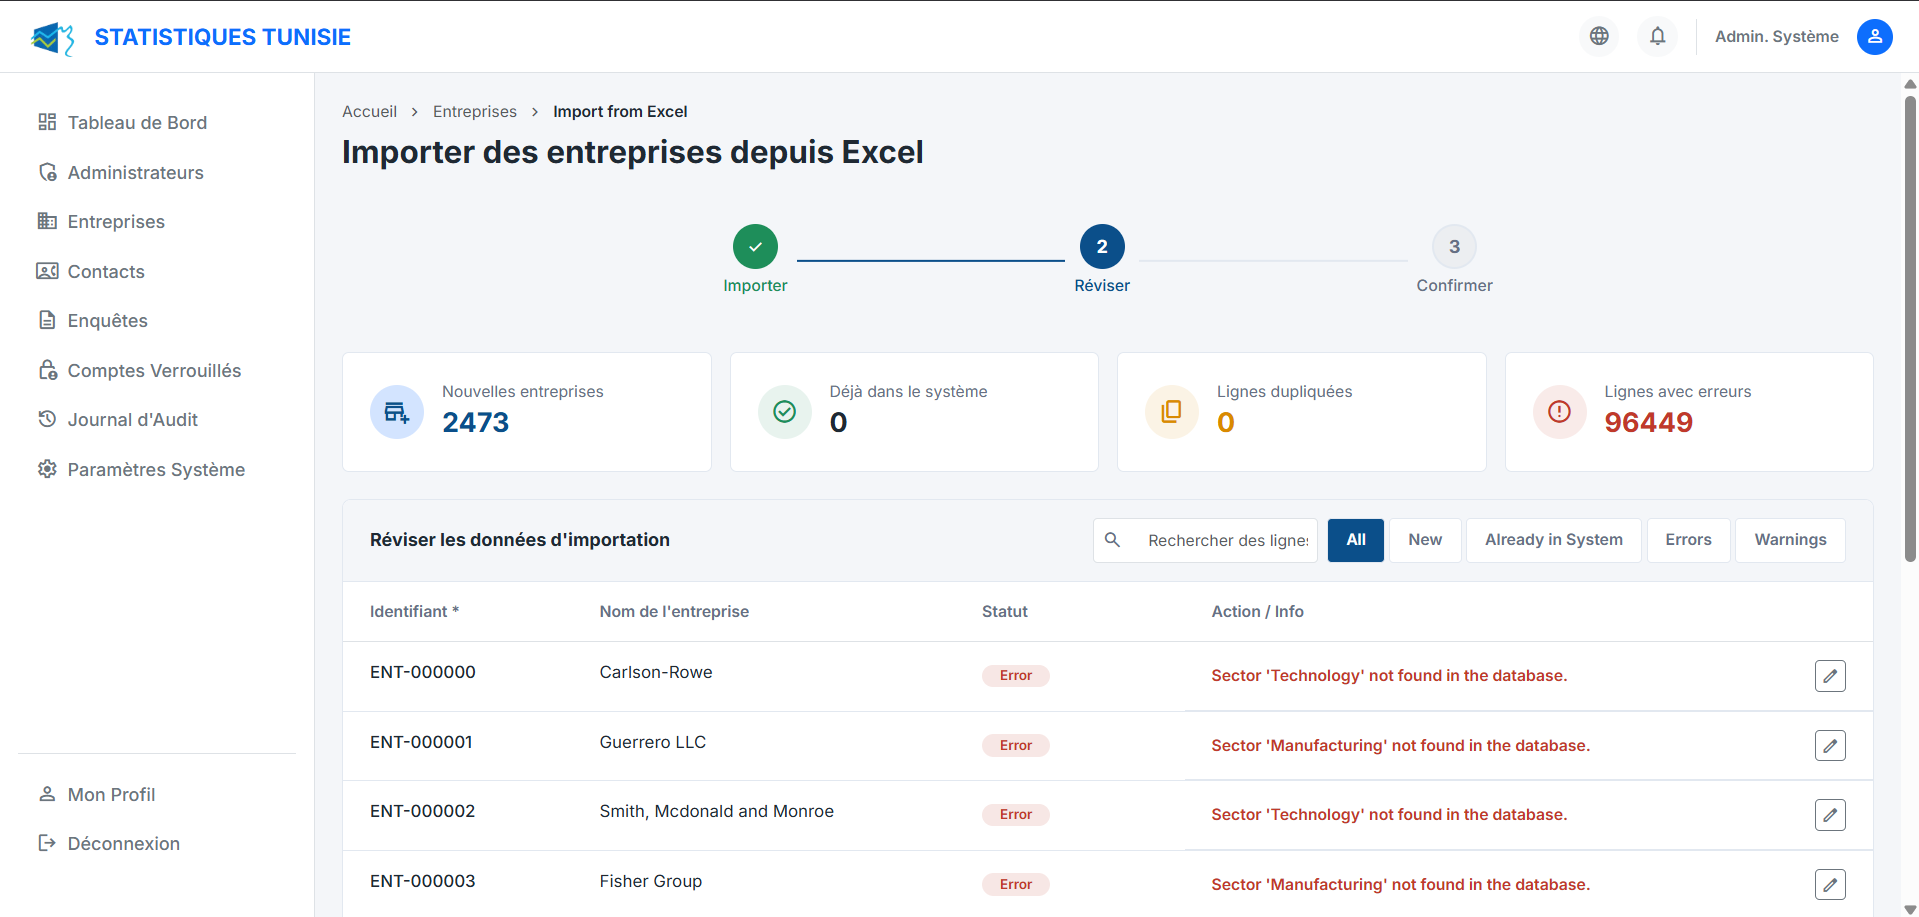
\includegraphics[width=1.1\textwidth]{images/screenshots/sprint0/batch_import_2nd_step.png}}
    \caption{Batch Import – Data Validation, showing results of a controlled synthetic stress test with a deliberately injected majority of error rows to validate the pipeline's per-row error reporting under adversarial conditions.}
    \label{fig:ui_batch_validate}
\end{figure}

To validate the reliability of the asynchronous company import pipeline prior to production use, a synthetic dataset generator was developed using \texttt{openpyxl}'s write-only streaming mode, enabling files of realistic scale ($\approx$100MB) to be produced without exhausting memory during generation. The generator accepts parameters controlling the exact distribution of valid, warning, error, and duplicate rows, producing reproducible, ground-truth-labeled test files for stress testing under adversarial conditions. Listing \ref{lst:celery_import} highlights the Celery task logic for asynchronous bulk spreadsheet processing.

\begin{lstlisting}[language=Python, caption={Asynchronous Company Import Task Excerpt (\texttt{app/tasks/import\_tasks.py})}, label={lst:celery_import}]
@celery_app.task
def process_excel_import(session_id: str, file_path: str):
    db: Session = SessionLocal()
    try:
        session = db.query(ImportSession).filter(
            ImportSession.id == session_id
        ).first()
        wb = openpyxl.load_workbook(
            file_path, read_only=True, data_only=True
        )
        ws = wb.active
        # Read and validate rows into staging table
        for i, row_vals in enumerate(data_rows, start=2):
            staging_records.append(CompanyImportStaging(...))
            if len(staging_records) >= 2000:
                db.bulk_save_objects(staging_records)
                db.commit()
                staging_records = []
    finally:
        db.close()
\end{lstlisting}

\begin{figure}[H]
    \centering
    \makebox[\textwidth][c]{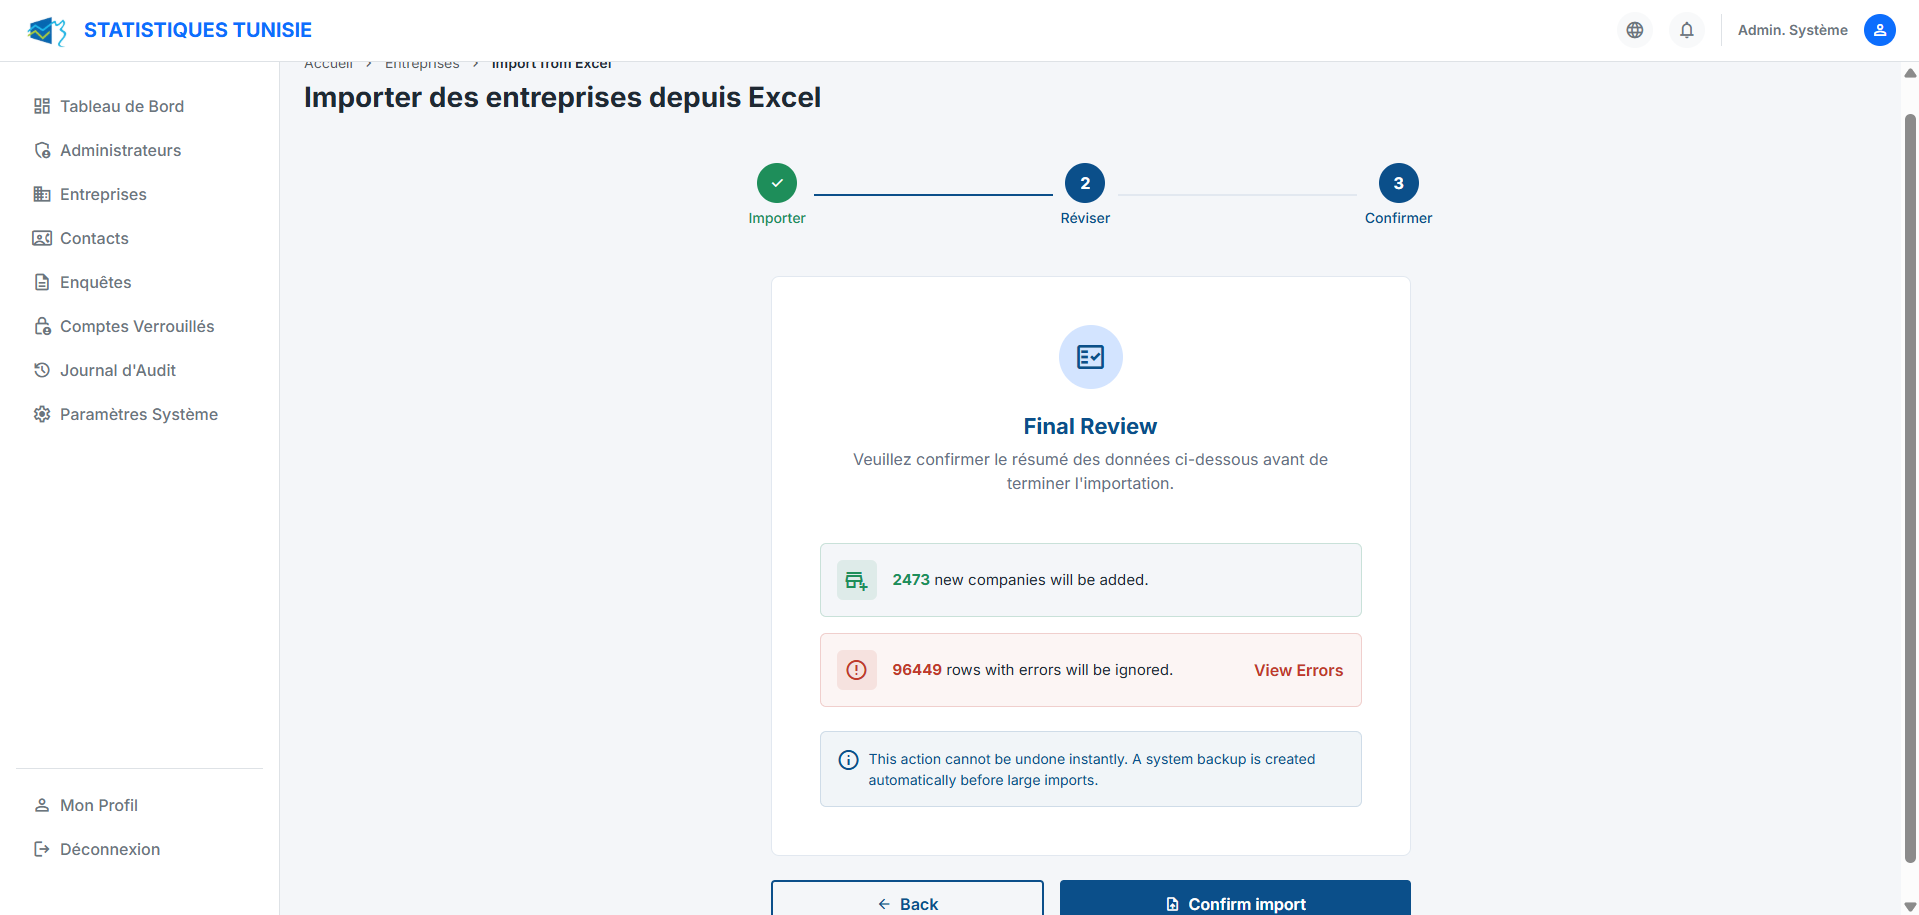
\includegraphics[width=1.1\textwidth]{images/screenshots/sprint0/batch_import_final_step.png}}
    \caption{Batch Import - Processing}
    \label{fig:ui_batch_processing}
\end{figure}

\newpage
\subsection{Manage surveys Interface}
The survey management interface enables administrators and survey managers to comprehensively configure statistical campaigns, define passage periods, assign company samples, and monitor results.

\begin{figure}[H]
    \centering
    \makebox[\textwidth][c]{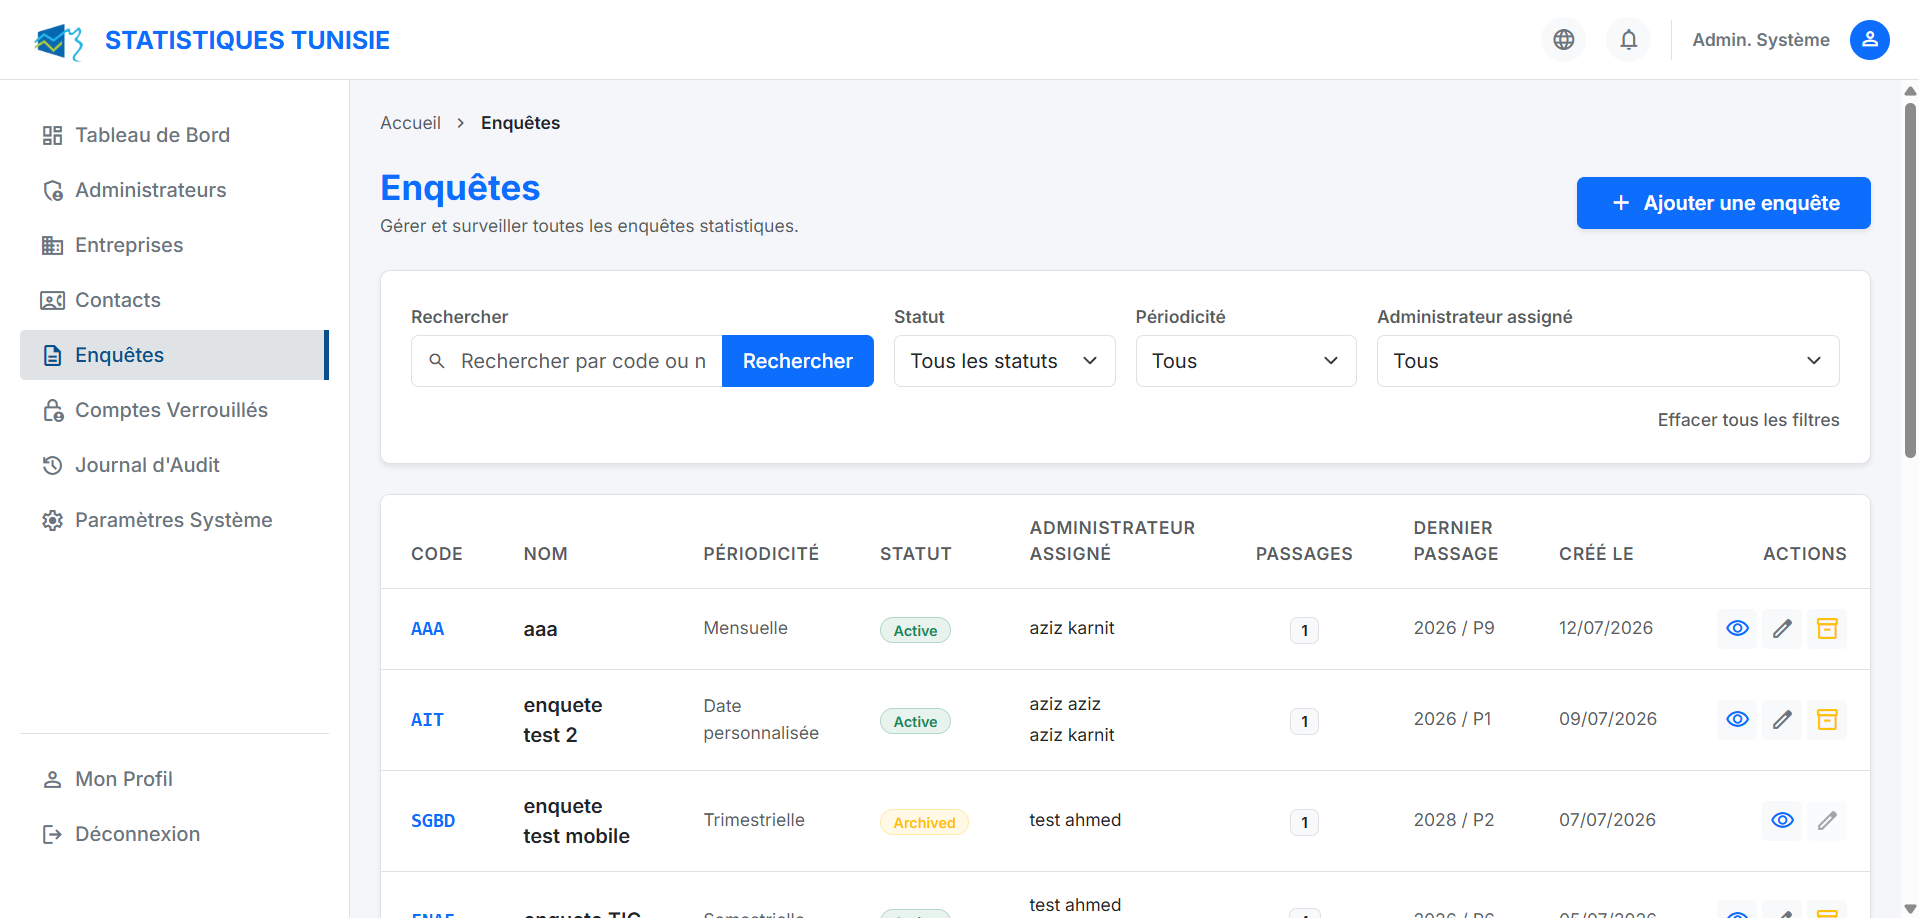
\includegraphics[width=1.1\textwidth]{images/screenshots/sprint0/survey_page.png}}
    \caption{Survey Directory Interface}
    \label{fig:ui_survey_page}
\end{figure}

\begin{figure}[H]
    \centering
    \makebox[\textwidth][c]{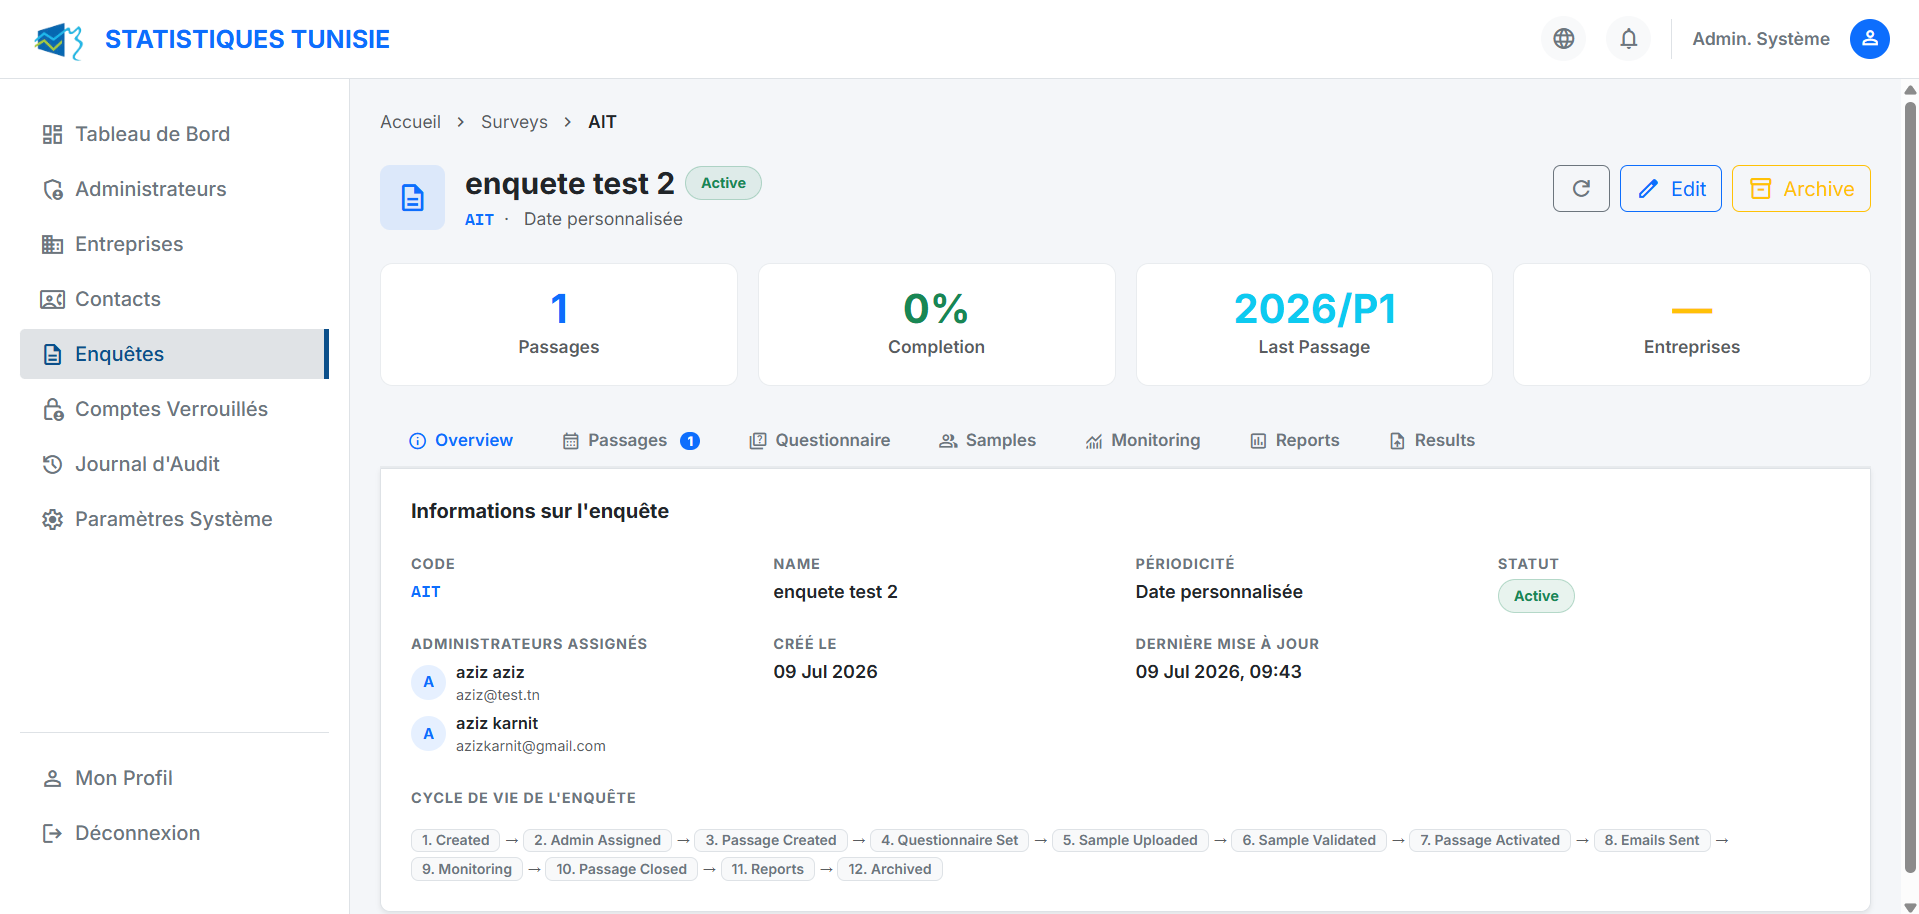
\includegraphics[width=1.1\textwidth]{images/screenshots/sprint0/survey_overview.png}}
    \caption{Survey Overview Dashboard}
    \label{fig:ui_survey_overview}
\end{figure}

\begin{figure}[H]
    \centering
    \makebox[\textwidth][c]{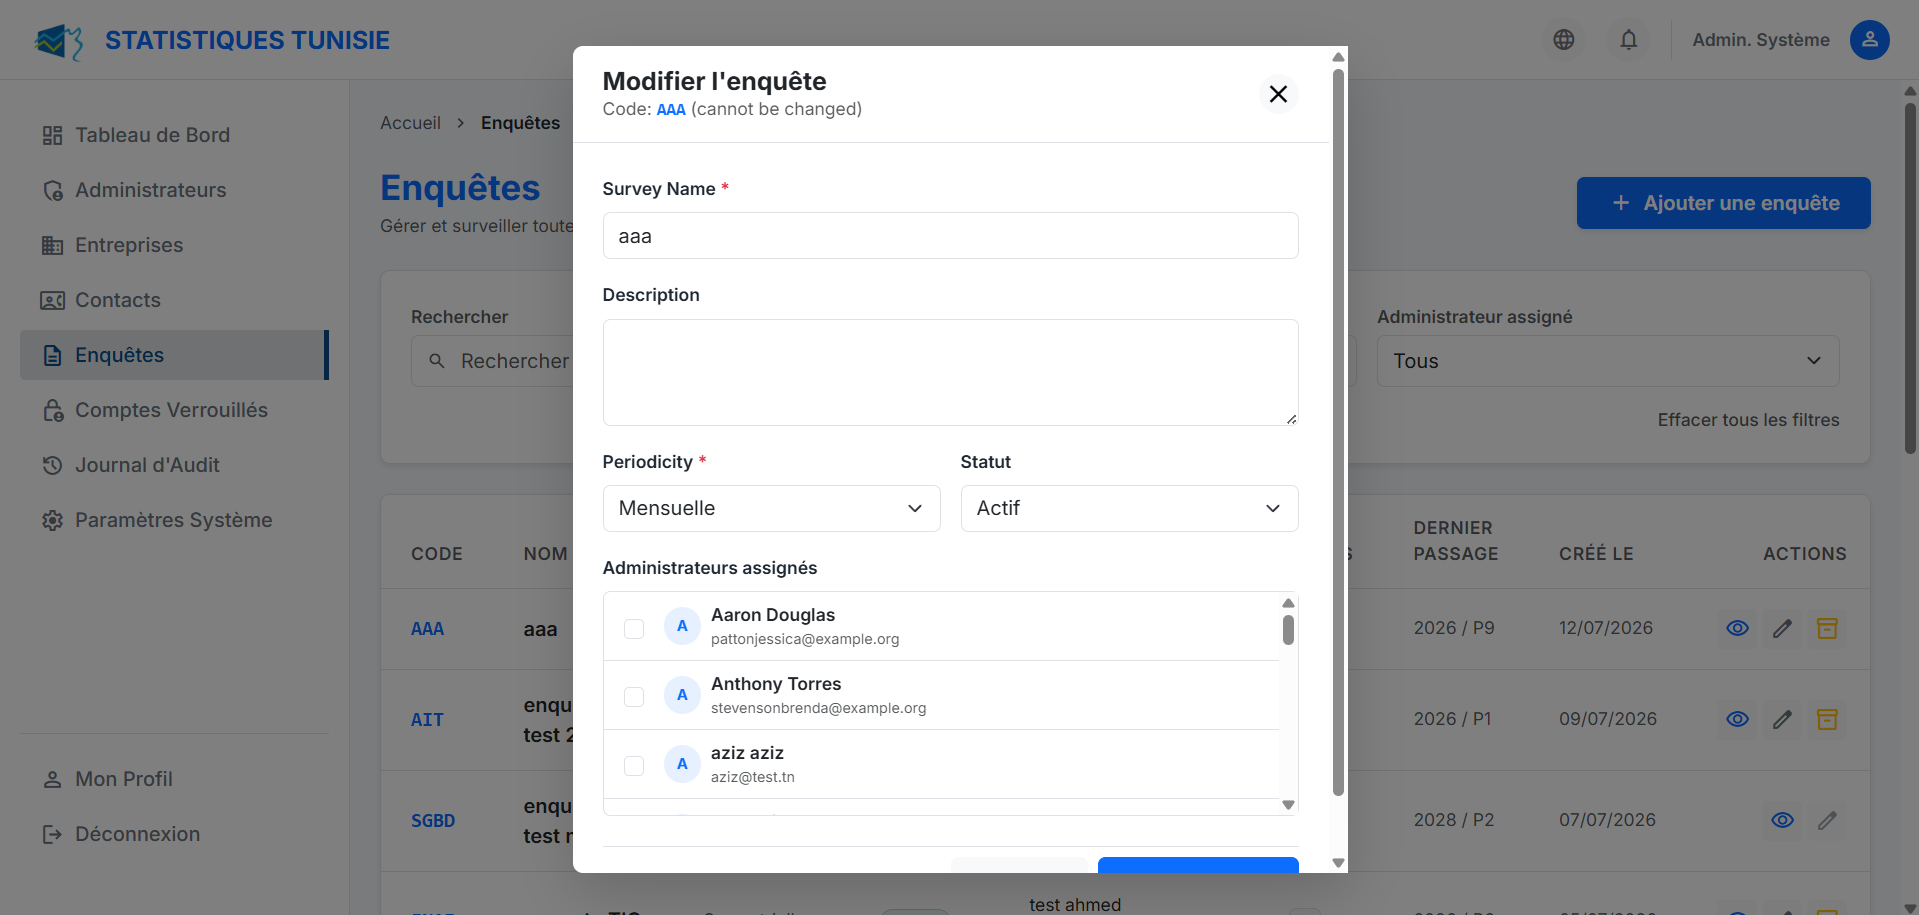
\includegraphics[width=1.1\textwidth]{images/screenshots/sprint0/edit_survey.png}}
    \caption{Edit Survey Configuration}
    \label{fig:ui_edit_survey}
\end{figure}

\begin{figure}[H]
    \centering
    \makebox[\textwidth][c]{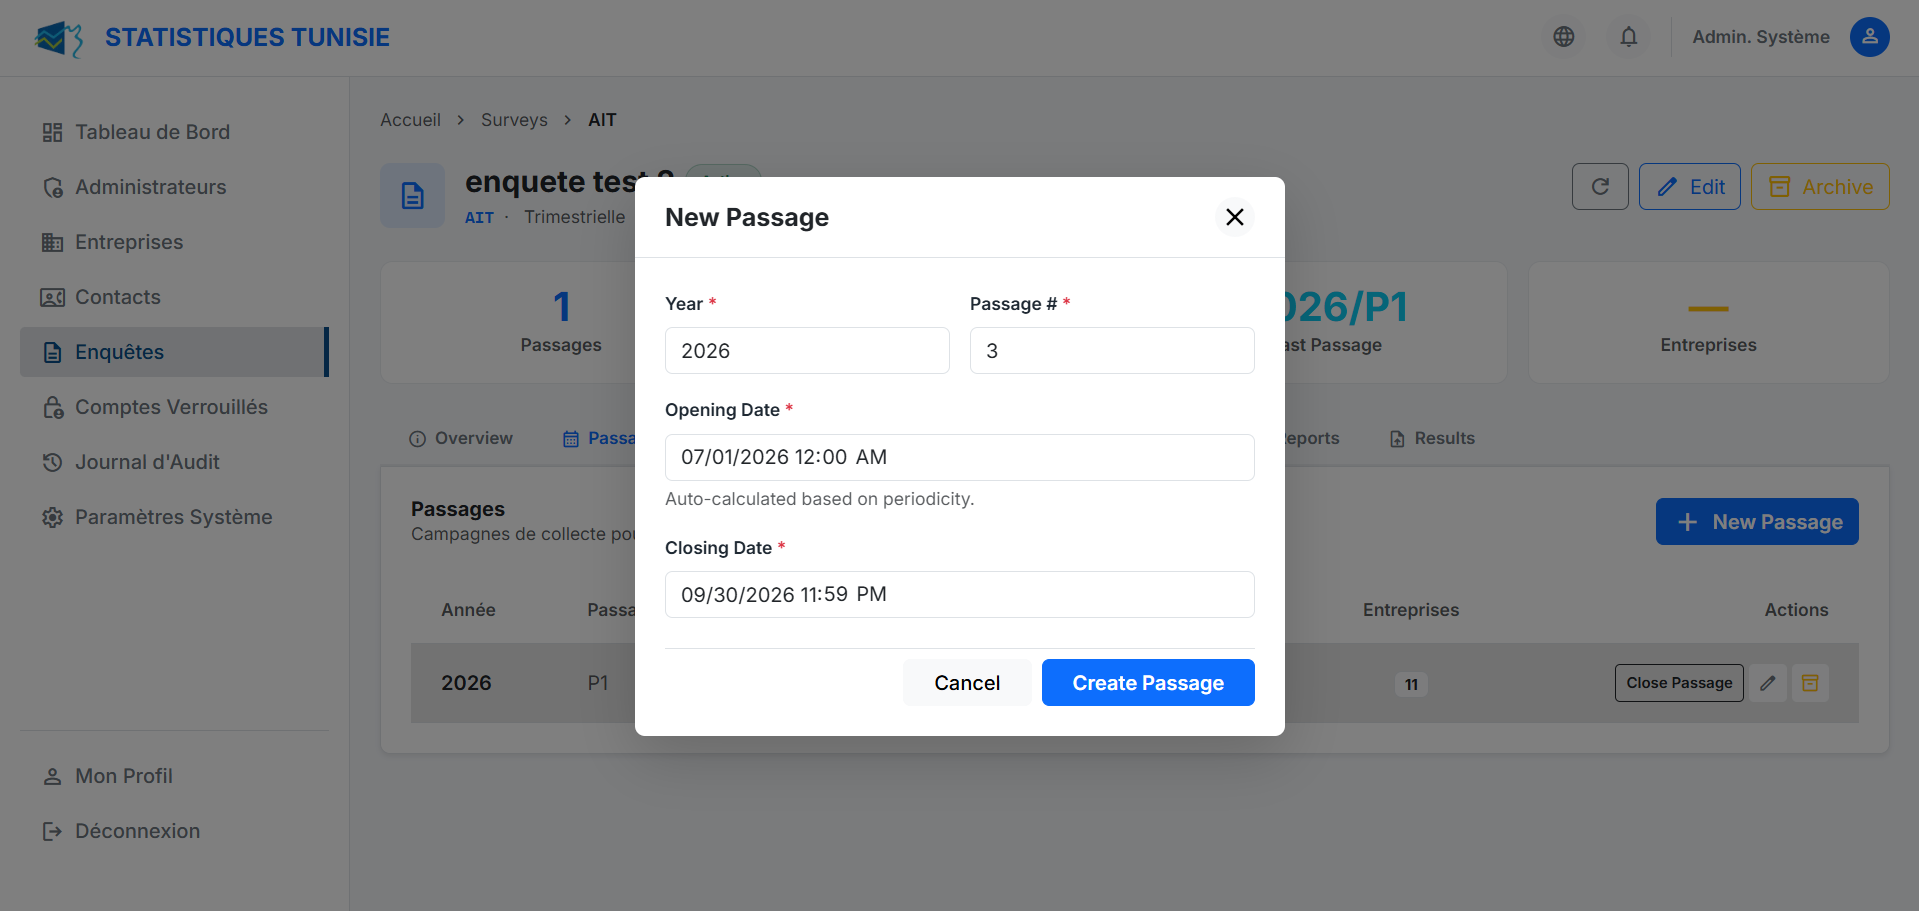
\includegraphics[width=1.1\textwidth]{images/screenshots/sprint0/add_passage.png}}
    \caption{Add Survey Passage Form}
    \label{fig:ui_add_passage}
\end{figure}

\begin{figure}[H]
    \centering
    \makebox[\textwidth][c]{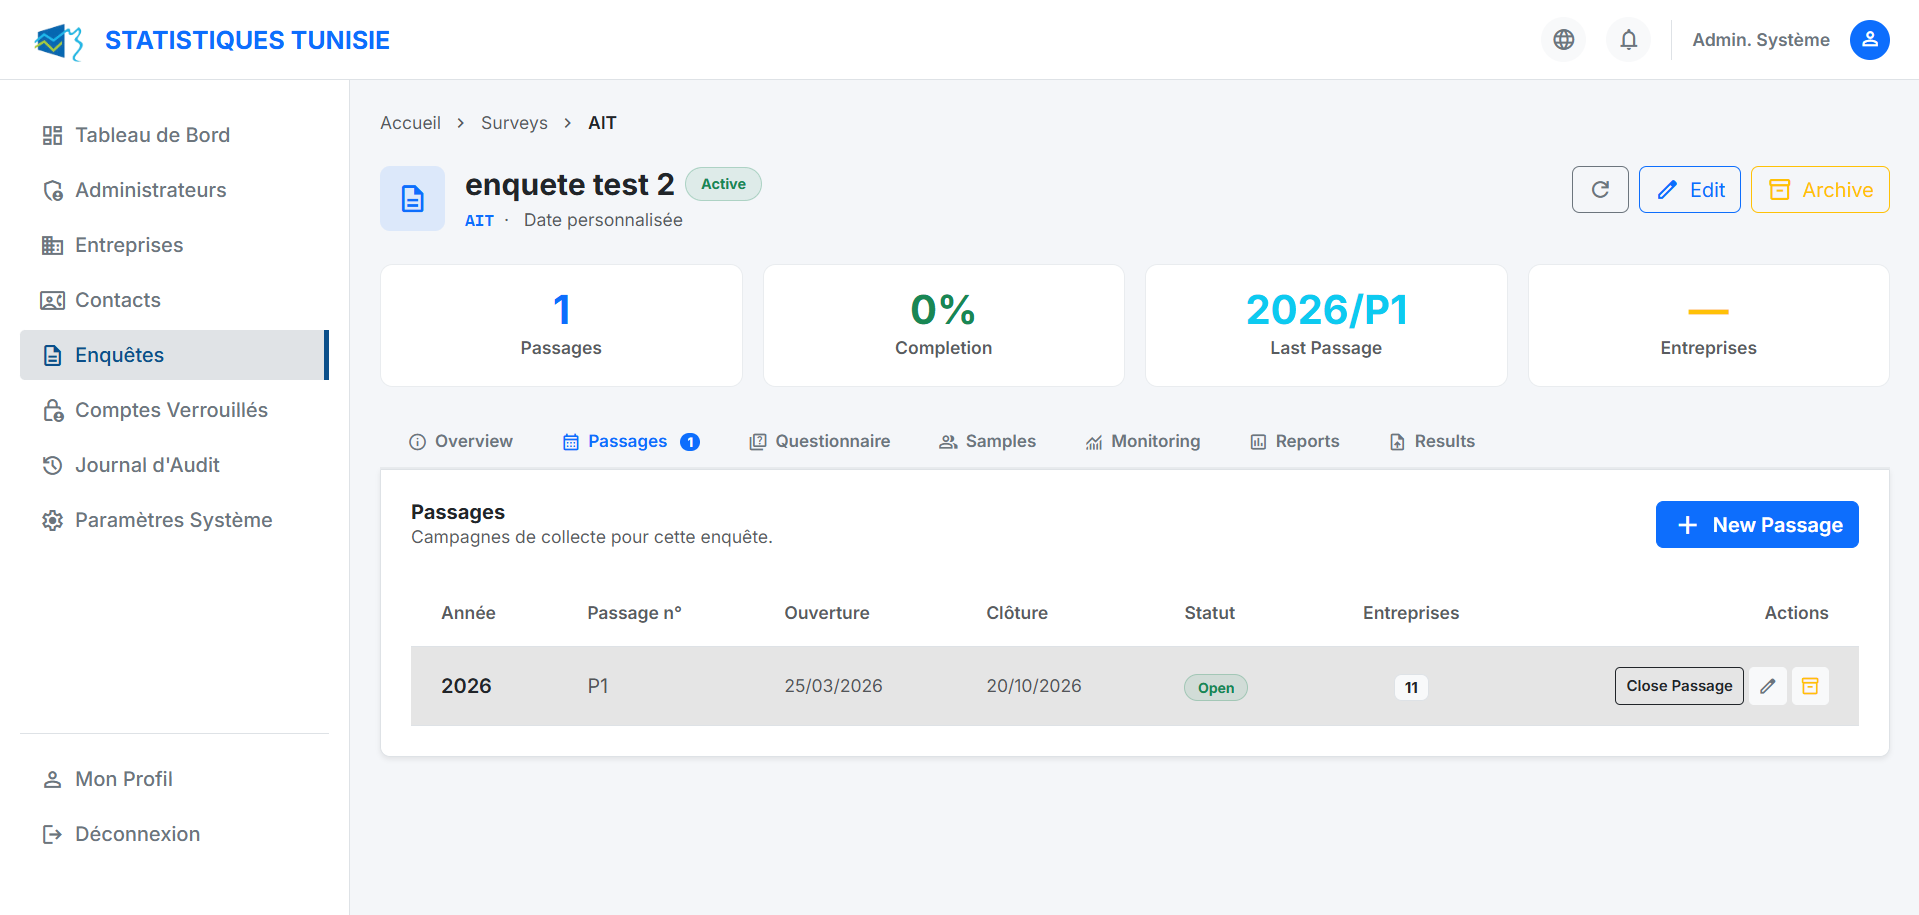
\includegraphics[width=1.1\textwidth]{images/screenshots/sprint0/survey_passage.png}}
    \caption{Survey Passage Details}
    \label{fig:ui_survey_passage}
\end{figure}

\begin{figure}[H]
    \centering
    \makebox[\textwidth][c]{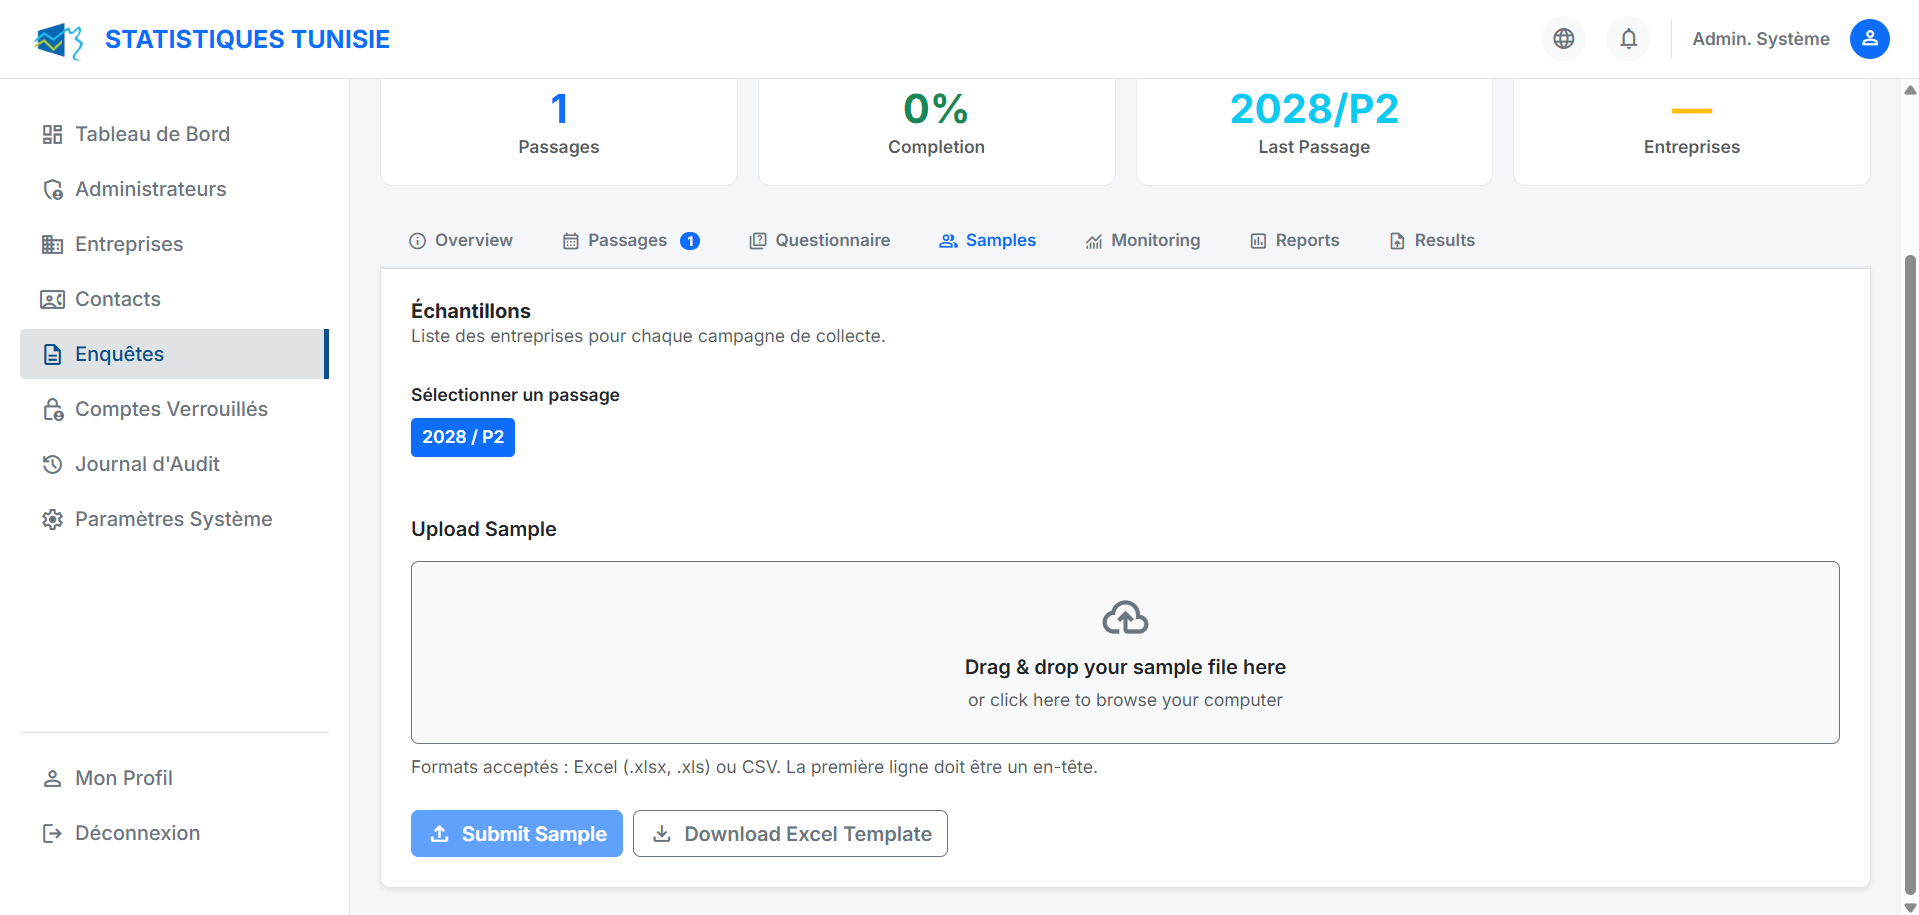
\includegraphics[width=1.1\textwidth]{images/screenshots/sprint0/sample_page.png}}
    \caption{Company Sample Assignment Interface}
    \label{fig:ui_sample_page}
\end{figure}

\begin{figure}[H]
    \centering
    \makebox[\textwidth][c]{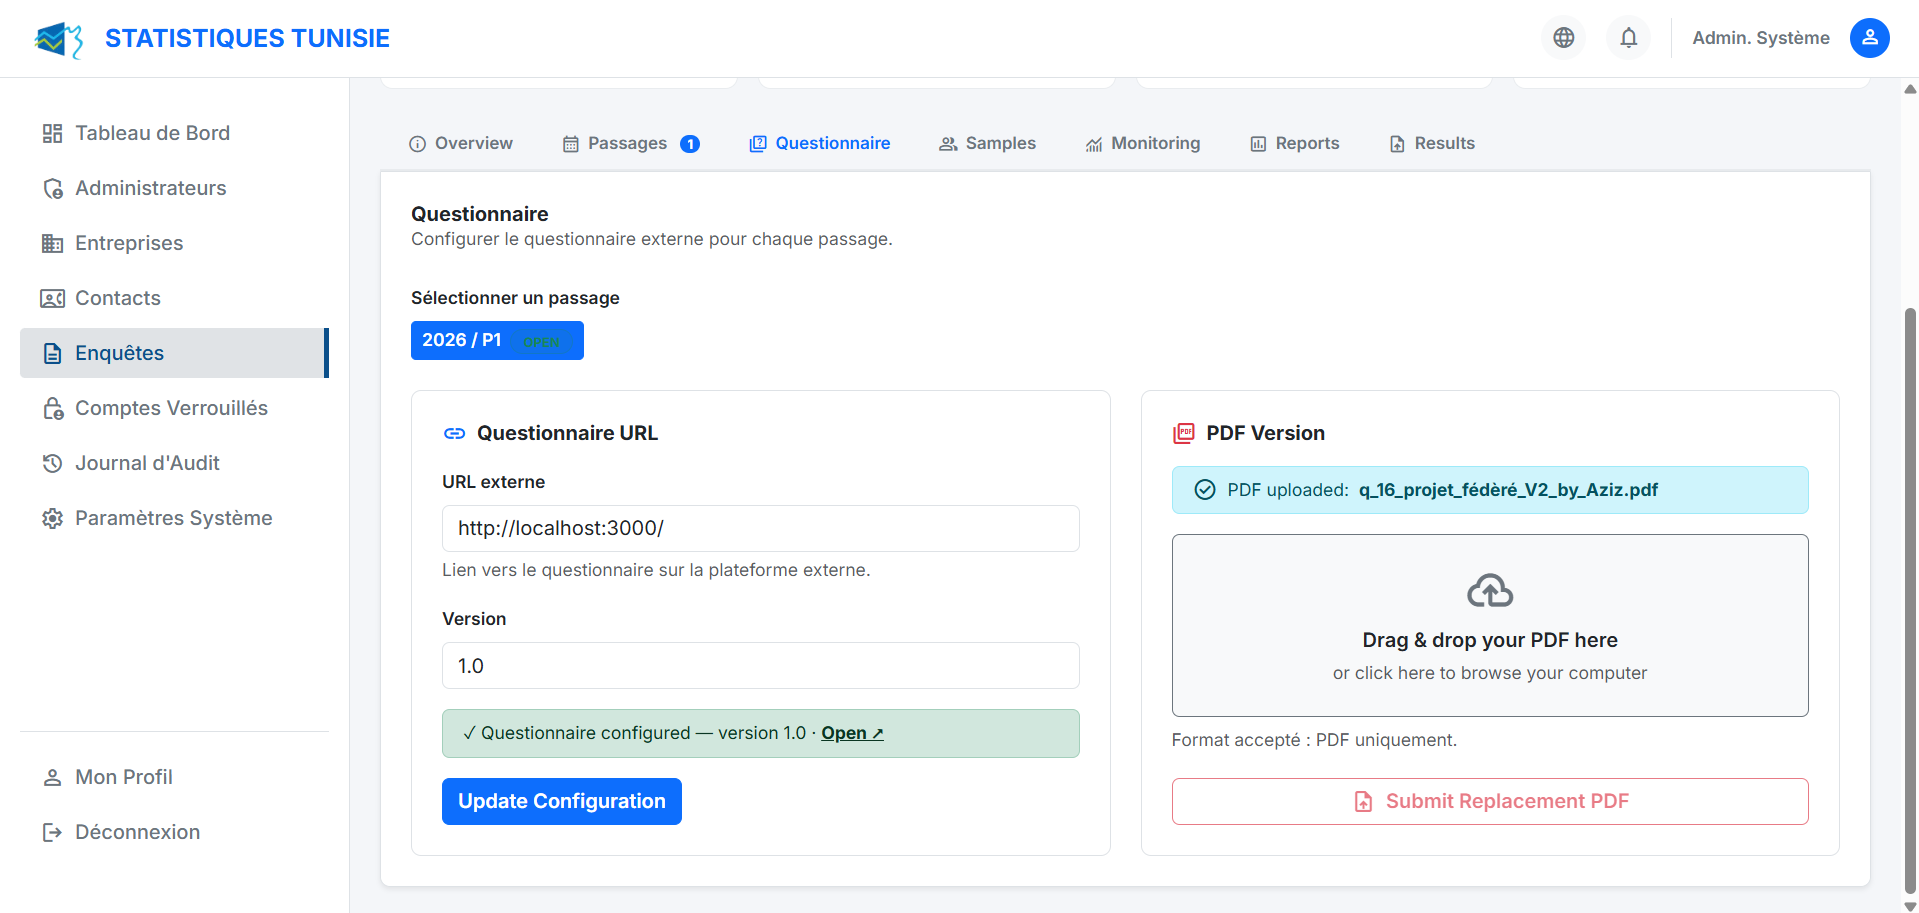
\includegraphics[width=1.1\textwidth]{images/screenshots/sprint0/questionnaire_page.png}}
    \caption{Questionnaire Template Management}
    \label{fig:ui_questionnaire_page}
\end{figure}

\begin{figure}[H]
    \centering
    \makebox[\textwidth][c]{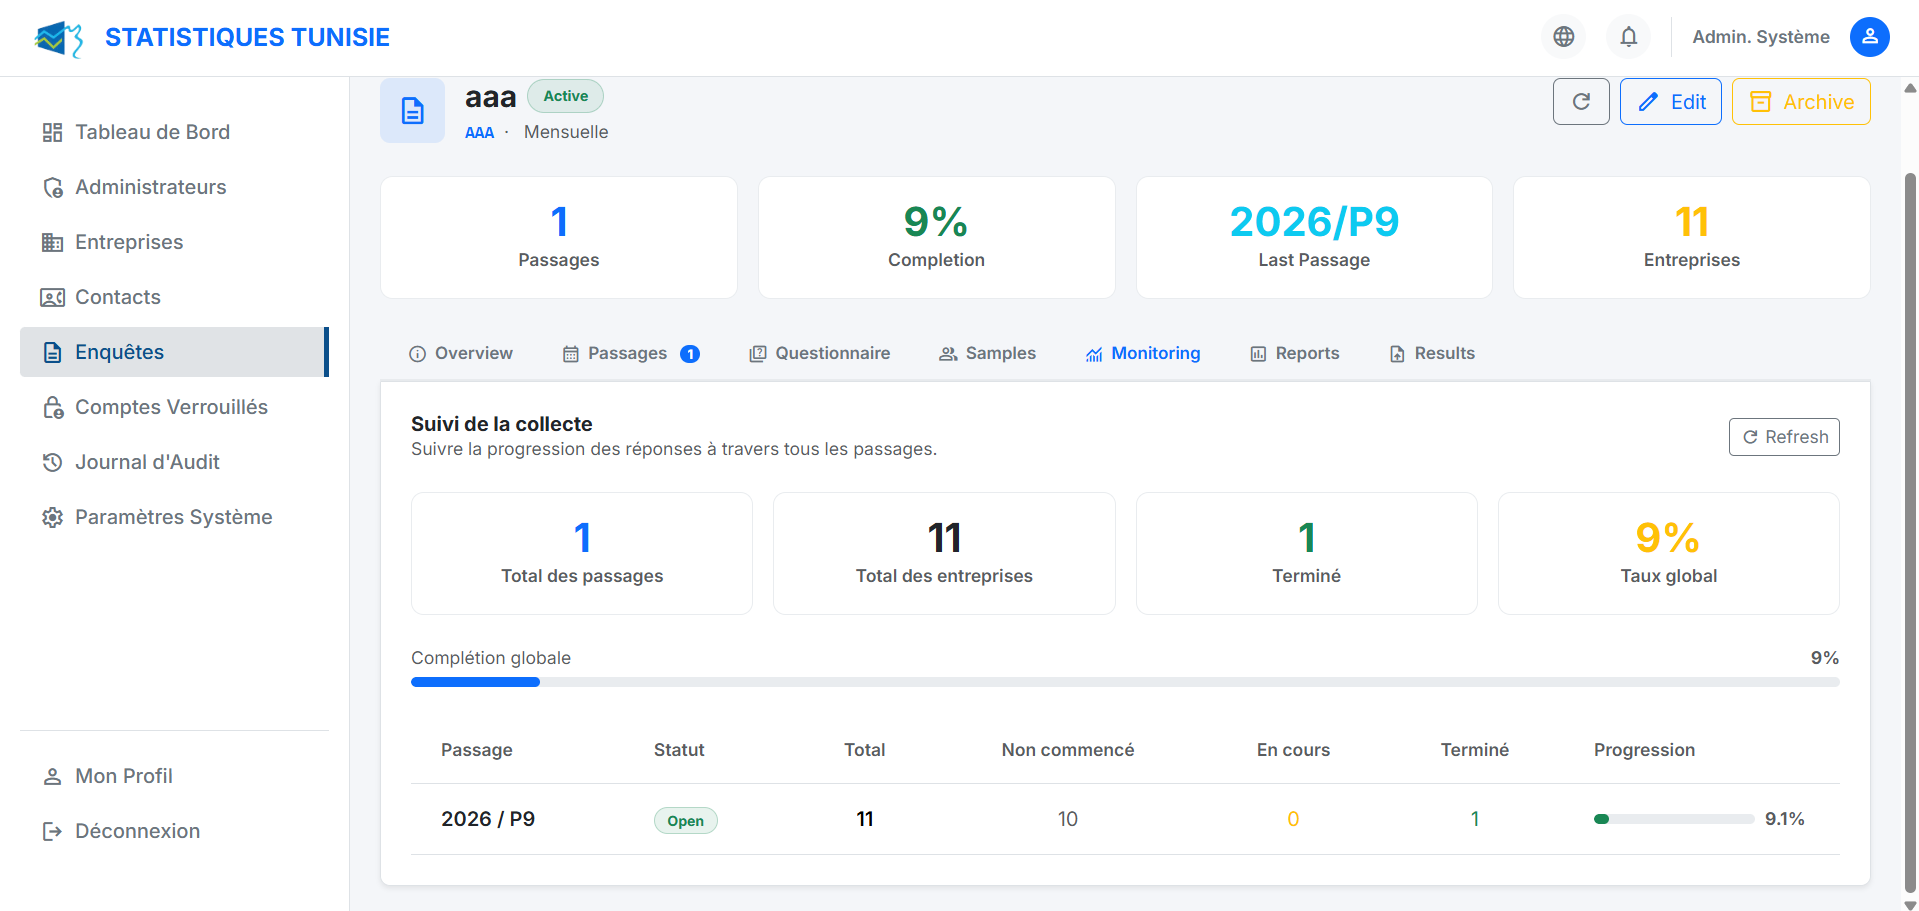
\includegraphics[width=1.1\textwidth]{images/screenshots/sprint0/monitoring_page.png}}
    \caption{Survey Passage Monitoring Dashboard}
    \label{fig:ui_monitoring}
\end{figure}

\begin{figure}[H]
    \centering
    \makebox[\textwidth][c]{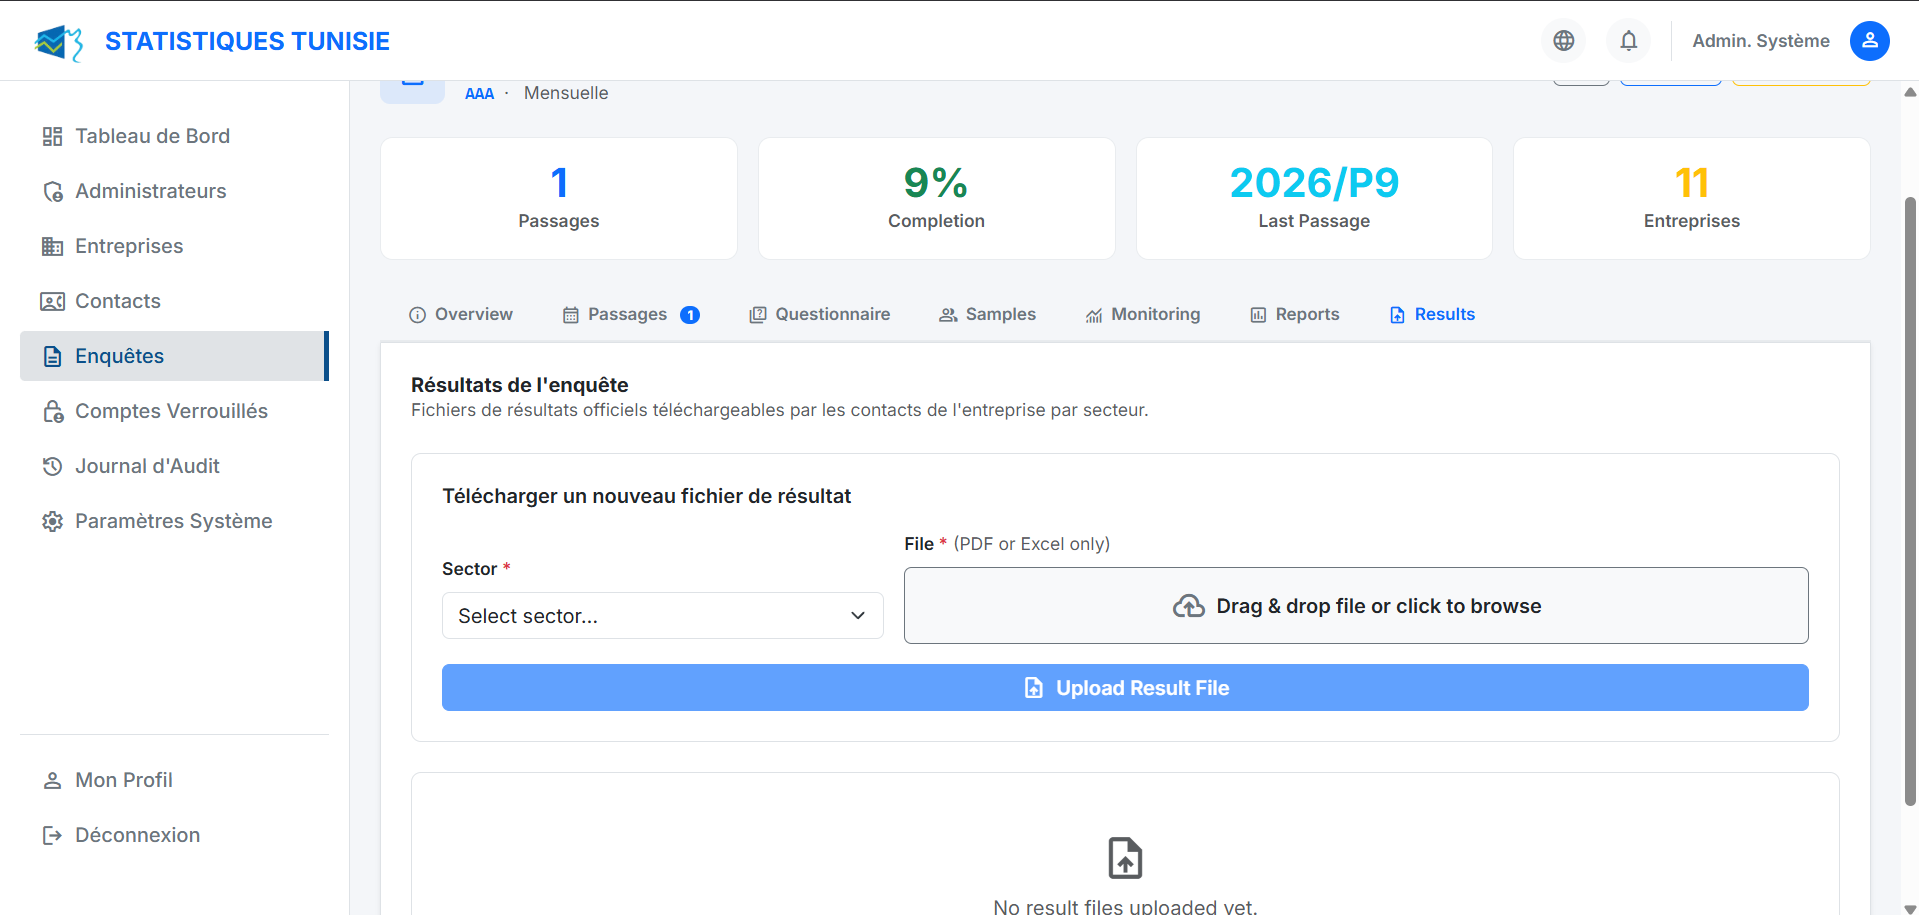
\includegraphics[width=1.1\textwidth]{images/screenshots/sprint0/results_page.png}}
    \caption{Survey Results Interface}
    \label{fig:ui_results}
\end{figure}


\section{Sprint 0 Conclusion}
In this chapter, we detailed the development of Sprint 0, which established the authentication system and core administrative management features of the platform. We presented the sprint backlog, refined each use case with detailed textual specifications, designed structural and sequence models, and demonstrated the implemented user interfaces. As noted in sprint retrospectives, fine-tuning the 2FA OTP expiration and Redis account lockout synchronization required additional validation iterations beyond initial estimates.

All planned user stories for Sprint 0 (``Login'', ``Manage admins'', ``Manage contacts'', ``Manage companies'', and ``Manage surveys'') were successfully developed and integrated, establishing a solid foundation for the platform. In the next chapter, we will address Sprint 1, focusing on survey administration and contact survey submission portals.

\newpage
\chapter{Sprint 1 -- Survey Portals \& Account Management}

\section{Introduction}
This chapter covers the development of Sprint 1, which focuses on the core survey submission portal for company contacts and additional secondary administrative features. It details the sprint backlog, the refinement of each user story, dynamic flow models, and the implementation of the user interfaces.

\section{Sprint 1 Backlog}
The Sprint 1 backlog encompasses the functional requirements assigned to the first development cycle following the setup of the core administration portal.

\begin{table}[H]
\centering
\caption{Sprint 1 Backlog}
\label{tab:sprint1_backlog}
\vspace{0.15cm}
\small
\renewcommand{\arraystretch}{1.15}
\begin{tabular}{|c|p{10.5cm}|c|}
\hline
\textbf{ID} & \textbf{User Story} & \textbf{Priority} \\ \hline
US06 & As a Company Contact, I want to Consult assigned surveys to view my active questionnaires. & High \\ \hline
US07 & As a Company Contact, I want to Consult assigned results to check my past survey responses. & High \\ \hline
US08 & As a System Administrator, I want to Manage system settings to configure global parameters. & Medium \\ \hline
US09 & As a System Administrator or Account Manager, I want to Manage locked accounts to restore or restrict system access. & Medium \\ \hline
US10 & As a user, I want to Manage profile to modify my personal contact information. & Low \\ \hline
\end{tabular}
\end{table}

\newpage
\section{Sprint 1 Refinement}
In this section, we refine the functional details and textual specifications for the use cases of Sprint 1.

\subsection{Refinement of the Use Case ``Consult assigned surveys''}
The diagram below illustrates the refinement of the ``Consult assigned surveys'' use case and its interactions with system actors:

\begin{figure}[H]
    \centering
    \makebox[\textwidth][c]{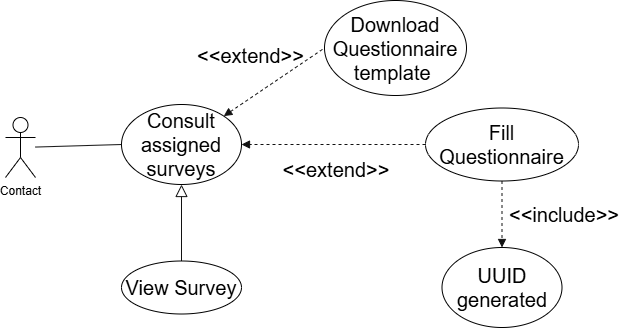
\includegraphics[width=1\textwidth]{images/out/diagrams/use case/assign_survey.png}}
    \caption{Use Case Diagram -- Consult assigned surveys}
    \label{fig:uc_consult_surveys}
\end{figure}

\newpage
Table \ref{tab:refinement_consult_surveys} presents the textual description of the ``Consult assigned surveys'' use case:

\begin{table}[H]
\centering
\caption{Textual description -- Consult assigned surveys}
\label{tab:refinement_consult_surveys}
\vspace{0.2cm}
\small
\renewcommand{\arraystretch}{1.15}
\begin{tabular}{|p{3.5cm}|p{12.0cm}|}
\hline
\textbf{Use Case} & Consult assigned surveys \\ \hline
\textbf{Actor} & Company Contact \\ \hline
\textbf{Pre-condition} & The Company Contact is authenticated and active on the platform. \\ \hline
\textbf{Post-condition} & The contact can view active surveys, download the required reference templates, and upload their completed questionnaire. \\ \hline
\textbf{Main Scenario} & 
1. The contact receives an email notification upon being assigned to a survey passage. \newline
2. The contact navigates to the ``My Surveys'' portal. \newline
3. The system retrieves and lists all active survey passages assigned to the contact's company. \newline
4. The contact selects a specific survey passage to view details. \newline
5. The system displays passage deadlines and provides two options: ``Download Template'' and ``Fill Questionnaire''. \newline
6. (Optional) The contact downloads the template to prepare answers offline. \newline
7. The contact clicks ``Fill Questionnaire''. \newline
8. The system generates an anonymous UUID based on the contact and passage to ensure data confidentiality. \newline
9. The system redirects the contact to the external questionnaire system, passing the UUID. \newline
10. The contact fills the questionnaire in the external system (with the ability to save progress and return later). \\ \hline
\textbf{Alternative Scenarios} & 
$\bullet$ No active surveys: The system displays a message indicating no pending surveys are assigned. \newline
$\bullet$ External system unavailable: The platform displays a maintenance warning and asks the user to try again later. \\ \hline
\textbf{Exception} & Server connection drop during file upload; the system displays a network retry prompt. \\ \hline
\end{tabular}
\end{table}

\newpage
\subsection{Refinement of the Use Case ``Consult assigned results''}
The diagram below illustrates the refinement of the ``Consult assigned results'' use case and its interactions with system actors:

\begin{figure}[H]
    \centering
    \makebox[\textwidth][c]{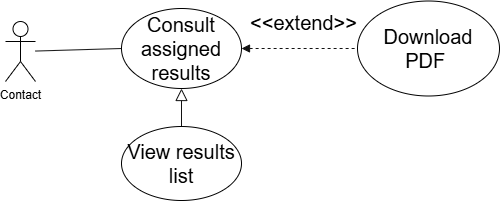
\includegraphics[width=1\textwidth]{images/out/diagrams/use case/consult results.png}}
    \caption{Use Case Diagram -- Consult assigned results}
    \label{fig:uc_consult_results}
\end{figure}

Table \ref{tab:refinement_consult_results} presents the textual description of the ``Consult assigned results'' use case:

\begin{table}[H]
\centering
\caption{Textual description -- Consult assigned results}
\label{tab:refinement_consult_results}
\vspace{0.2cm}
\small
\renewcommand{\arraystretch}{1.15}
\begin{tabular}{|p{3.5cm}|p{12.0cm}|}
\hline
\textbf{Use Case} & Consult assigned results \\ \hline
\textbf{Actor} & Company Contact \\ \hline
\textbf{Pre-condition} & The Company Contact is authenticated and has previously submitted surveys. \\ \hline
\textbf{Post-condition} & The contact successfully views historical submission data and validation feedback. \\ \hline
\textbf{Main Scenario} & 
1. The contact accesses the ``Survey Results'' section. \newline
2. The system retrieves past survey submissions associated with the contact's company. \newline
3. The system displays a list of past survey results containing: Survey Name, File Name, Format, Published Date, and an Action column. \newline
4. The contact clicks the ``Download'' action for a specific result. \newline
5. The system initiates the download of the submitted file. \\ \hline
\textbf{Alternative Scenarios} & 
$\bullet$ No past submissions: The system displays a ``No historical data'' placeholder. \\ \hline
\textbf{Exception} & Database timeout; the system prompts the user to refresh the page. \\ \hline
\end{tabular}
\end{table}

\subsection{Refinement of the Use Case ``Manage system settings''}
The diagram below illustrates the refinement of the ``Manage system settings'' use case and its interactions with system actors:

\begin{figure}[H]
    \centering
    \makebox[\textwidth][c]{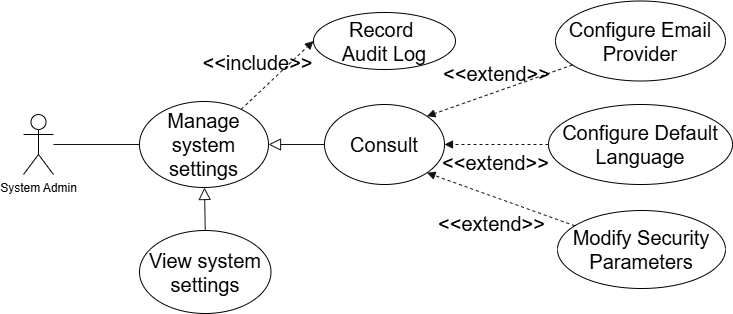
\includegraphics[width=0.89\textwidth]{images/out/diagrams/use case/system_settings.png}}
    \caption{Use Case Diagram -- Manage system settings}
    \label{fig:uc_manage_settings}
\end{figure}

Table \ref{tab:refinement_manage_settings} presents the textual description of the ``Manage system settings'' use case:

\begin{table}[H]
\centering
\caption{Textual description -- Manage system settings}
\label{tab:refinement_manage_settings}
\vspace{0.2cm}
\small
\renewcommand{\arraystretch}{1.15}
\begin{tabular}{|p{3.5cm}|p{12.0cm}|}
\hline
\textbf{Use Case} & Manage system settings \\ \hline
\textbf{Actor} & System Administrator \\ \hline
\textbf{Pre-condition} & The user is logged in as a System Administrator. \\ \hline
\textbf{Post-condition} & Global system parameters (Security protocols, Default Language, Email Provider) are securely updated. \\ \hline
\textbf{Main Scenario} & 
1. The administrator navigates to the ``System Settings'' dashboard. \newline
2. The system loads the current configuration parameters categorized by Security, Language, and Email. \newline
3. The administrator modifies a specific parameter value (e.g., 2FA code expiration, max login attempts, lockout duration, or default language). \newline
4. The administrator saves the new configuration. \newline
5. The system validates the numerical inputs and format constraints. \newline
6. The system updates the parameters in the database and refreshes the global application state. \newline
7. The system logs the configuration change in the audit trail. \\ \hline
\textbf{Alternative Scenarios} & 
$\bullet$ Invalid input format: The system rejects the change (e.g., providing a negative number for lockout duration) and displays a validation error. \\ \hline
\textbf{Exception} & Cache server unreachable; the system saves to DB but warns about delayed application. \\ \hline
\end{tabular}
\end{table}

\subsection{Refinement of the Use Case ``Manage locked accounts''}
The diagram below illustrates the refinement of the ``Manage locked accounts'' use case and its interactions with system actors:

\begin{figure}[H]
    \centering
    \makebox[\textwidth][c]{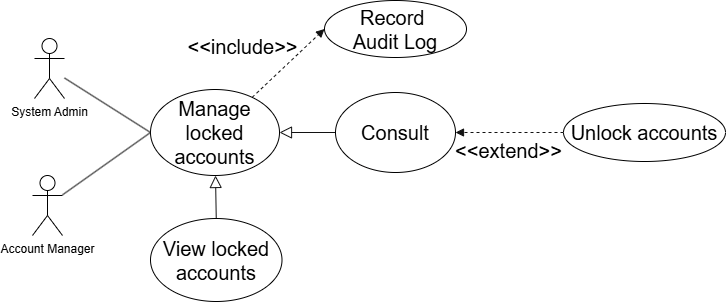
\includegraphics[width=1\textwidth]{images/out/diagrams/use case/unlocked_accounts.png}}
    \caption{Use Case Diagram -- Manage locked accounts}
    \label{fig:uc_manage_locked}
\end{figure}

Table \ref{tab:refinement_manage_locked} presents the textual description of the ``Manage locked accounts'' use case:

\begin{table}[H]
\centering
\caption{Textual description -- Manage locked accounts}
\label{tab:refinement_manage_locked}
\vspace{0.2cm}
\small
\renewcommand{\arraystretch}{1.15}
\begin{tabular}{|p{3.5cm}|p{12.0cm}|}
\hline
\textbf{Use Case} & Manage locked accounts \\ \hline
\textbf{Actor} & System Administrator, Account Manager \\ \hline
\textbf{Pre-condition} & The user has appropriate administrative privileges. \\ \hline
\textbf{Post-condition} & A user's account is unlocked, allowing them to authenticate, and the action is logged. \\ \hline
\textbf{Main Scenario} & 
1. The manager navigates to the ``Locked Accounts'' security monitoring interface. \newline
2. The system displays a list of accounts suspended due to multiple failed login attempts. \newline
3. The manager clicks ``Unlock'' on a specific user's row. \newline
4. The manager confirms the unlock action. \newline
5. The system resets the failed attempt counter and sets the account status to active. \newline
6. The system grants a temporary password-only login bypass window. \newline
7. The system records the unlock action in the security audit logs. \\ \hline
\textbf{Alternative Scenarios} & 
$\bullet$ Admin decides to permanently disable: The manager selects ``Disable permanently'' instead of unlocking. \\ \hline
\textbf{Exception} & Database timeout; the action fails and the manager is prompted to retry. \\ \hline
\end{tabular}
\end{table}

\subsection{Refinement of the Use Case ``Manage profile''}
The diagram below illustrates the refinement of the ``Manage profile'' use case and its interactions with system actors:

\begin{figure}[H]
    \centering
    \makebox[\textwidth][c]{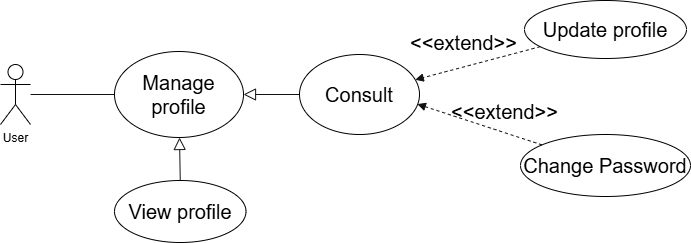
\includegraphics[width=1\textwidth]{images/out/diagrams/use case/manage profile.png}}
    \caption{Use Case Diagram -- Manage profile}
    \label{fig:uc_manage_profile}
\end{figure}

Table \ref{tab:refinement_manage_profile} presents the textual description of the ``Manage profile'' use case:

\begin{table}[H]
\centering
\caption{Textual description -- Manage profile}
\label{tab:refinement_manage_profile}
\vspace{0.2cm}
\small
\renewcommand{\arraystretch}{1.15}
\begin{tabular}{|p{3.5cm}|p{12.0cm}|}
\hline
\textbf{Use Case} & Manage profile \\ \hline
\textbf{Actor} & Any authenticated user \\ \hline
\textbf{Pre-condition} & The user is securely authenticated on the platform. \\ \hline
\textbf{Post-condition} & The user's personal details or password are updated in the database. \\ \hline
\textbf{Main Scenario} & 
1. The user clicks on their avatar and accesses the ``My Profile'' interface. \newline
2. The system loads the user's current personal data. \newline
3. The user modifies their phone number, interface language, or requests a password change. \newline
4. The user clicks ``Save Changes''. \newline
5. The system validates the input (e.g., verifying old password if changing to a new one). \newline
6. The system commits the changes to the database. \newline
7. The system displays a success confirmation message. \\ \hline
\textbf{Alternative Scenarios} & 
$\bullet$ Incorrect old password: The system rejects the password change request. \\ \hline
\textbf{Exception} & Session expiration during edit; user is redirected to login. \\ \hline
\end{tabular}
\end{table}

\section{Sprint 1 Conception}
This section presents the structural and dynamic design models for the use cases implemented in Sprint 1.

\subsection{Class Diagram -- Sprint 1 Core Domain}
The class diagram below models the entity structures, attributes, and relationships supporting the survey portal, responses, and user profile management:

\begin{figure}[H]
    \centering
    \makebox[\textwidth][c]{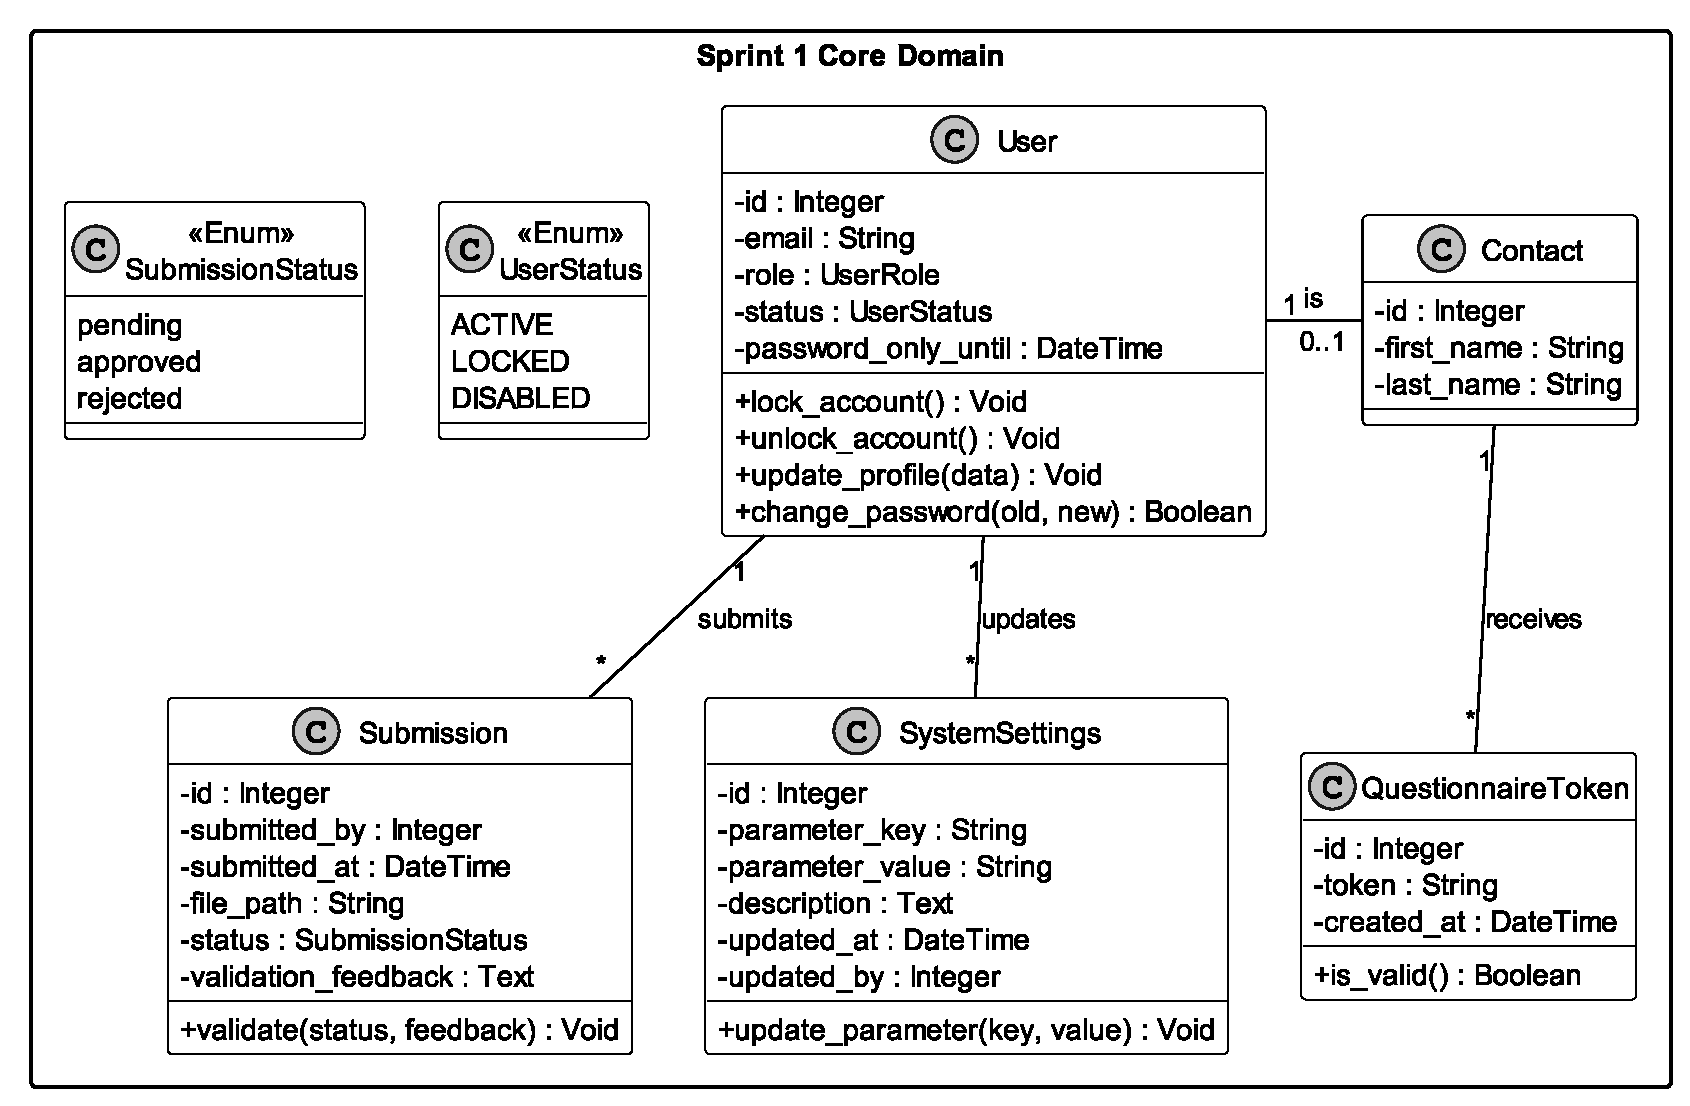
\includegraphics[width=1.2\textwidth]{images/out/diagrams/class/sprint1/sprint1.eps}}
    \caption{Sprint 1 Class Diagram}
    \label{fig:sprint1_class_diagram}
\end{figure}

The \texttt{Contact} class connects to \texttt{User} via the \texttt{is} association, establishing the link between a company contact profile and their corresponding login account in the system. The Sprint 1 class diagram (Figure \ref{fig:sprint1_class_diagram}) incorporates this association to support direct contact authentication, profile management, and dedicated survey dashboard access.

\newpage
\subsection{Sequence Diagram -- Use Case ``Consult assigned surveys''}
The diagram below illustrates the dynamic interactions for the ``Consult assigned surveys'' use case:

\begin{figure}[H]
    \centering
    \makebox[\textwidth][c]{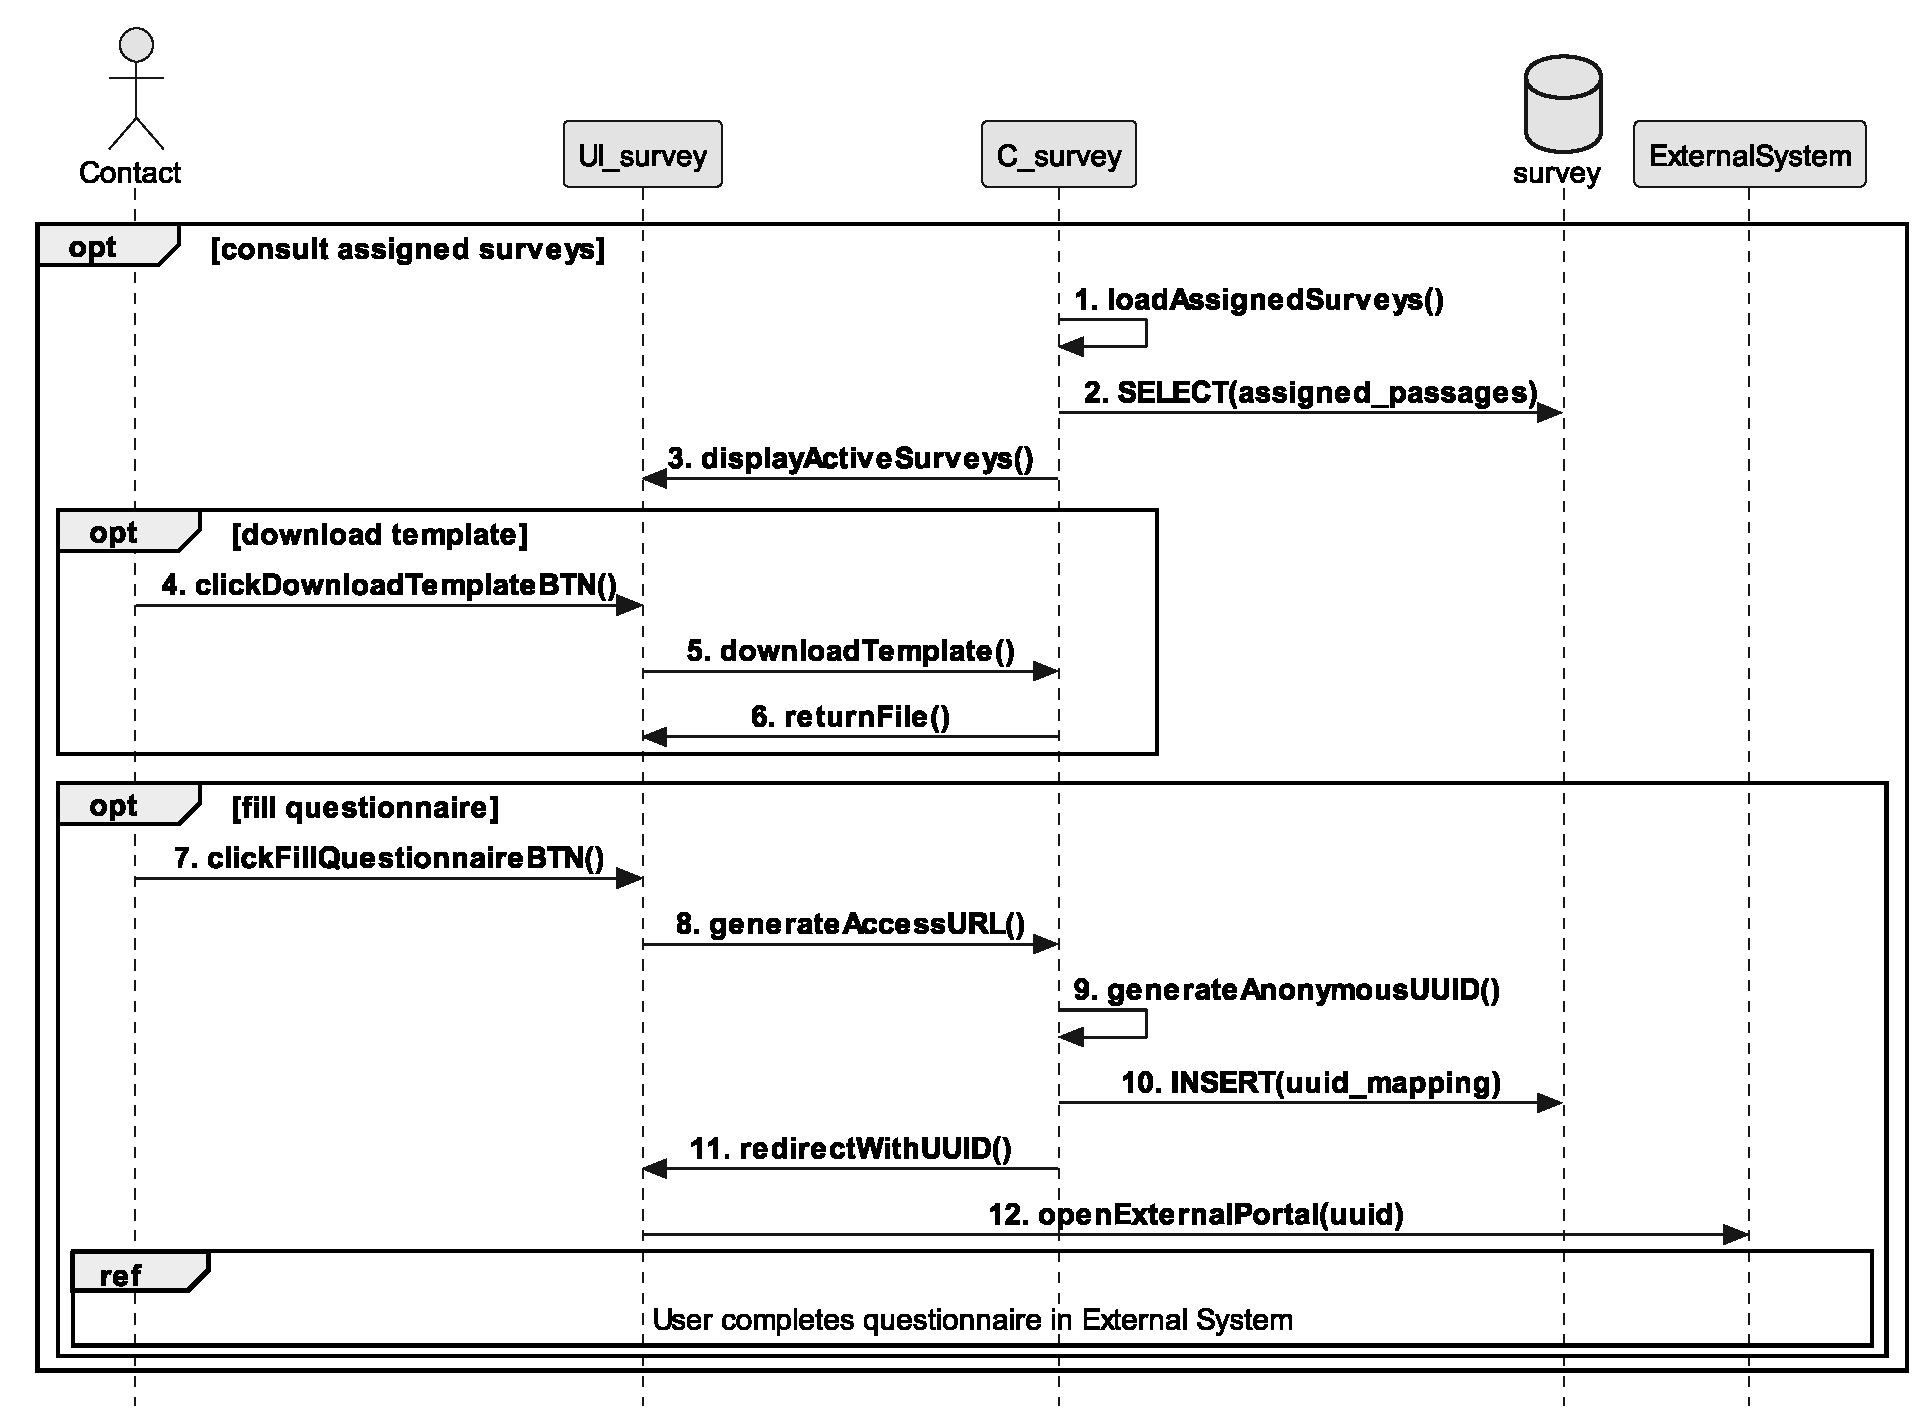
\includegraphics[width=1.2\textwidth]{images/out/diagrams/seq/consult_surveys/consult_surveys.eps}}
    \caption{Sequence Diagram -- Consult assigned surveys}
    \label{fig:seq_consult_surveys}
\end{figure}

\newpage
\subsection{Sequence Diagram -- Use Case ``Consult assigned results''}
The diagram below illustrates the dynamic interactions for the ``Consult assigned results'' use case:

\begin{figure}[H]
    \centering
    \makebox[\textwidth][c]{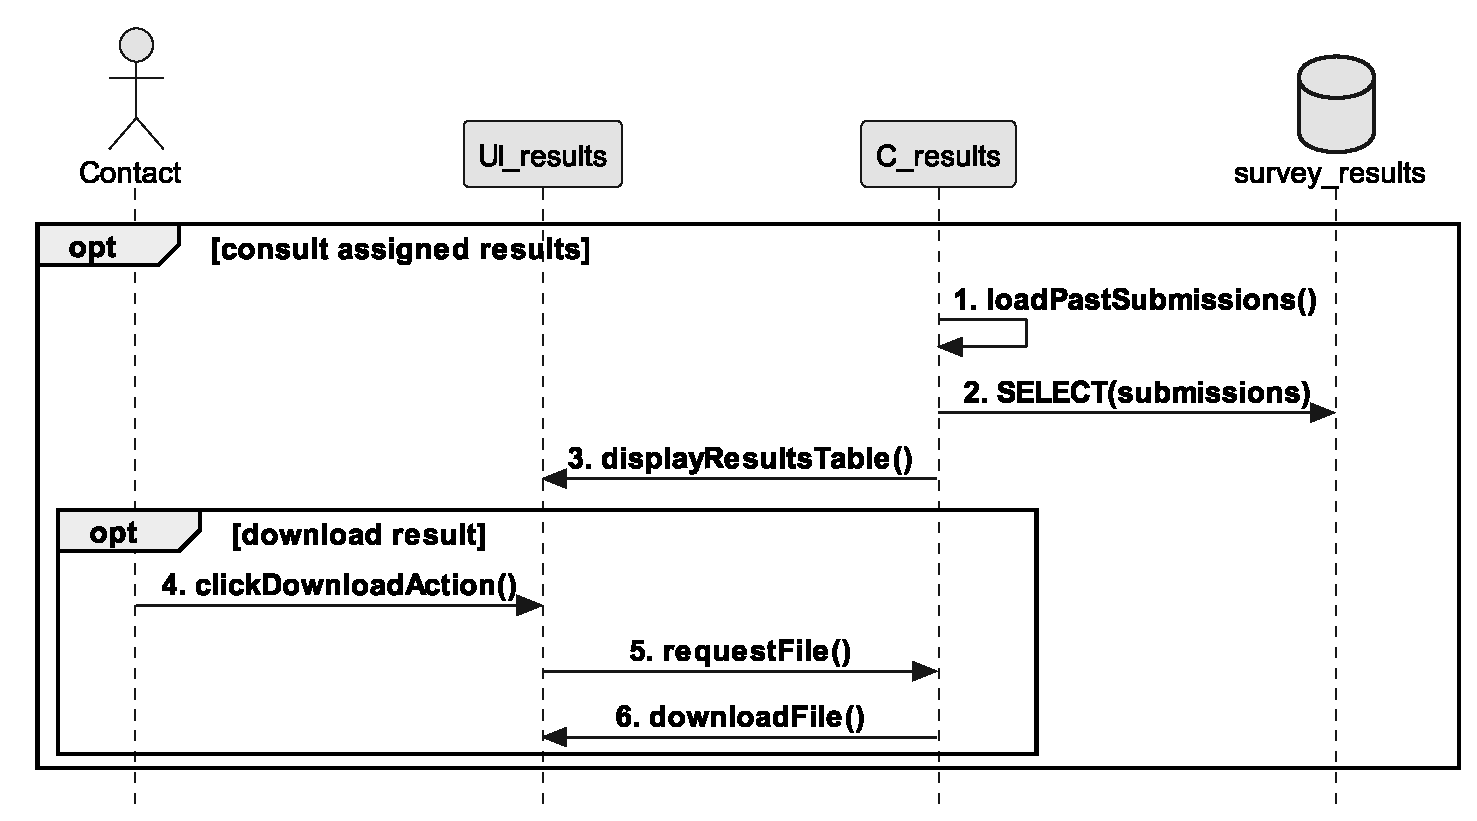
\includegraphics[width=1.2\textwidth]{images/out/diagrams/seq/consult_results/consult_results.eps}}
    \caption{Sequence Diagram -- Consult assigned results}
    \label{fig:seq_consult_results}
\end{figure}

\newpage
\subsection{Sequence Diagram -- Use Case ``Manage system settings''}
The diagram below illustrates the dynamic interactions for the ``Manage system settings'' use case:

\begin{figure}[H]
    \centering
    \makebox[\textwidth][c]{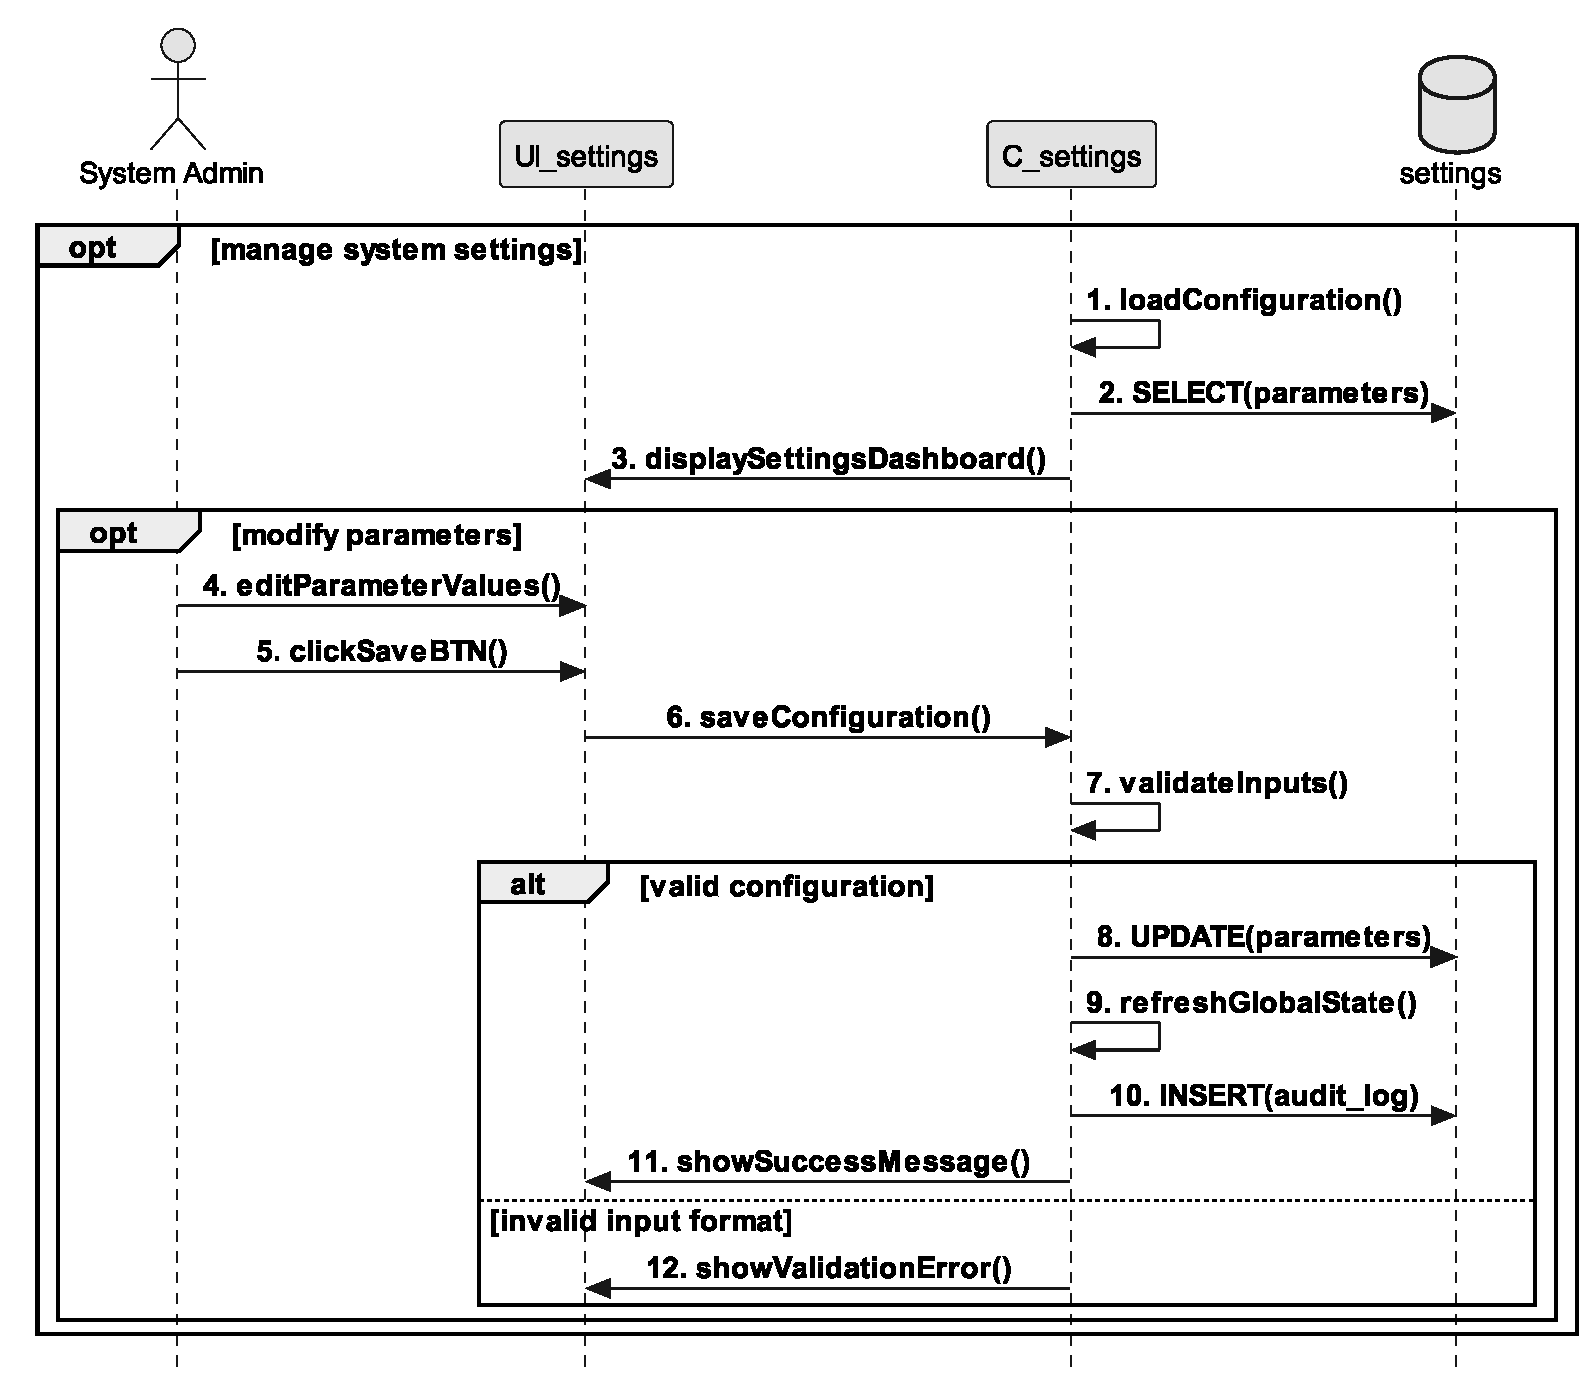
\includegraphics[width=1.2\textwidth]{images/out/diagrams/seq/system_settings/system_settings.eps}}
    \caption{Sequence Diagram -- Manage system settings}
    \label{fig:seq_manage_settings}
\end{figure}

\newpage
\subsection{Sequence Diagram -- Use Case ``Manage locked accounts''}
The diagram below illustrates the dynamic interactions for the ``Manage locked accounts'' use case:

\begin{figure}[H]
    \centering
    \makebox[\textwidth][c]{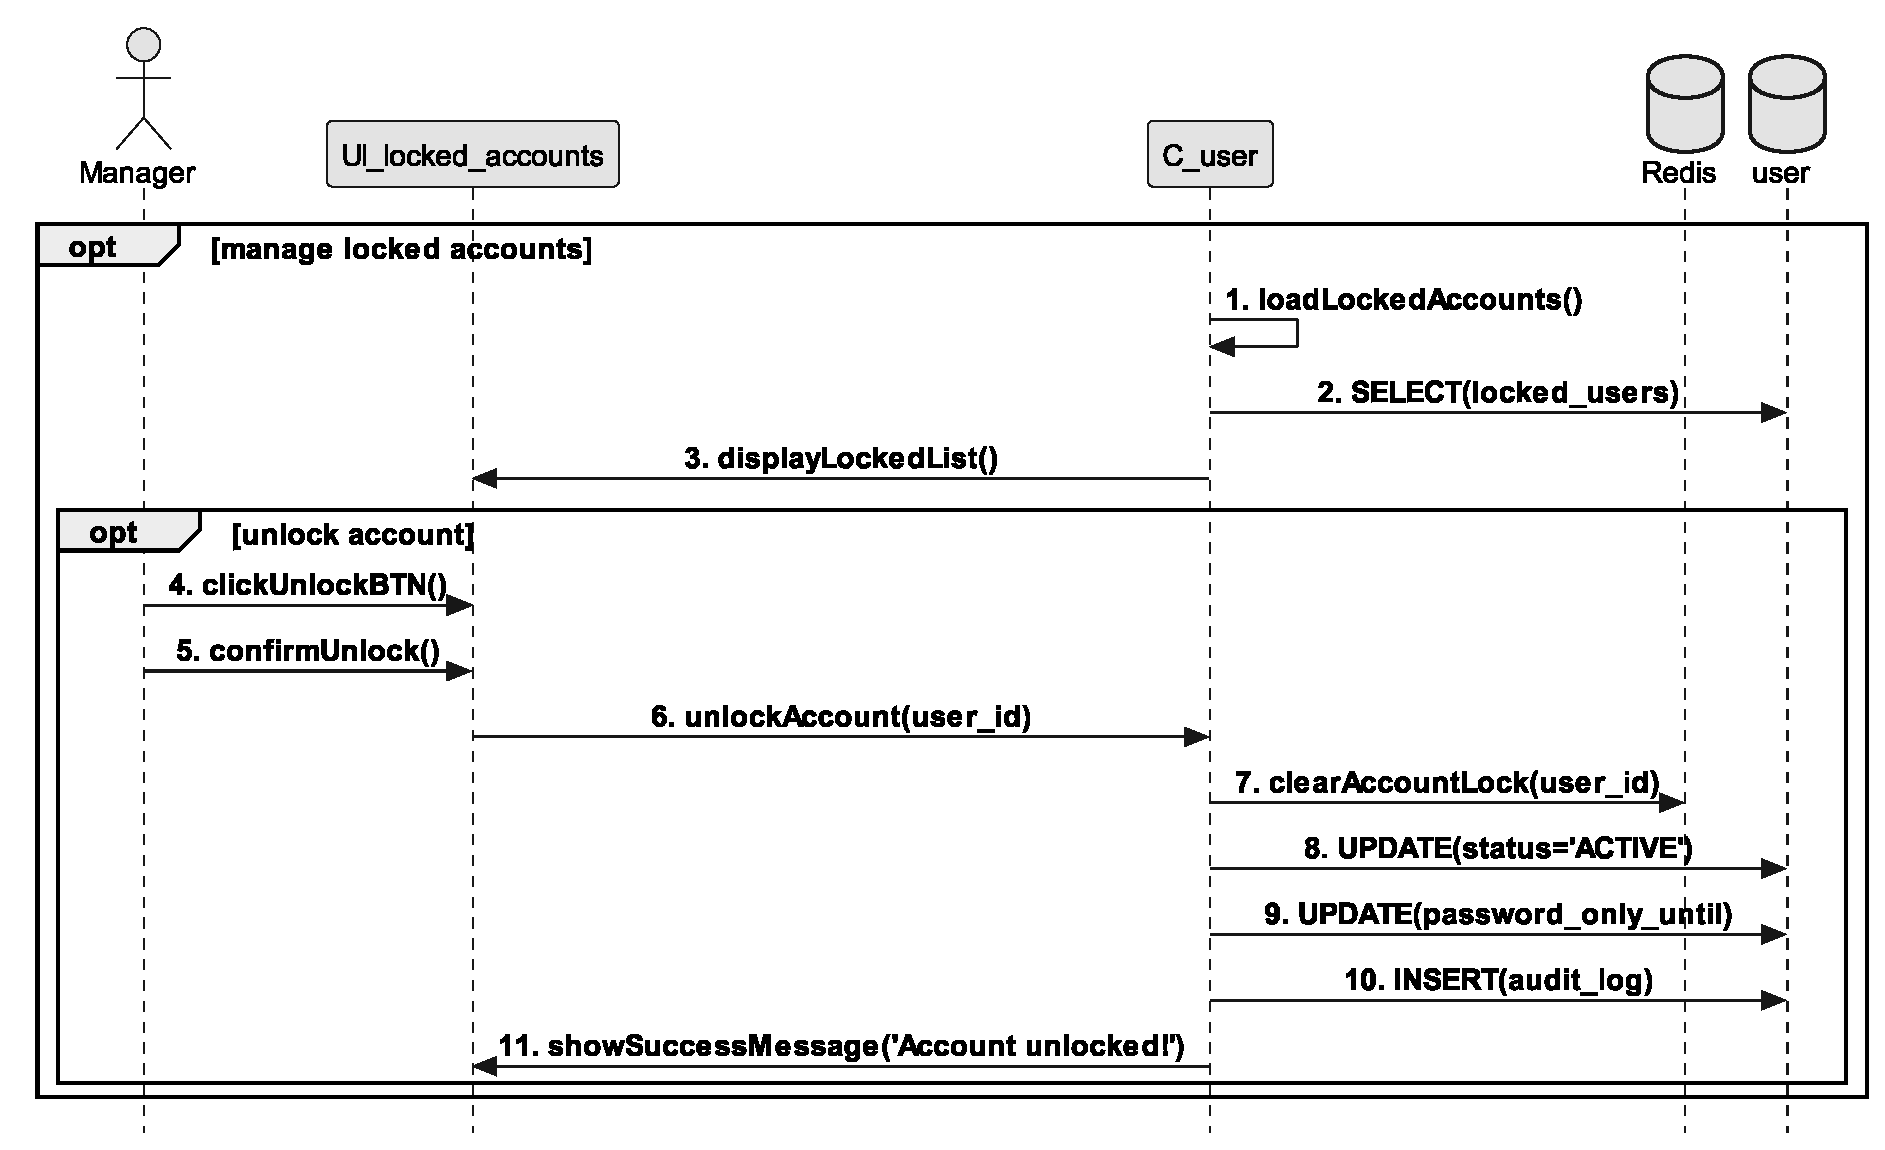
\includegraphics[width=1.2\textwidth]{images/out/diagrams/seq/manage_locked_accounts/manage_locked_accounts.eps}}
    \caption{Sequence Diagram -- Manage locked accounts}
    \label{fig:seq_manage_locked}
\end{figure}

\newpage
\subsection{State Diagram -- Use Case ``Manage locked accounts''}
The state diagram below illustrates the lifecycle and state transitions of an account during lockout and unlocking:

\begin{figure}[H]
    \centering
    \makebox[\textwidth][c]{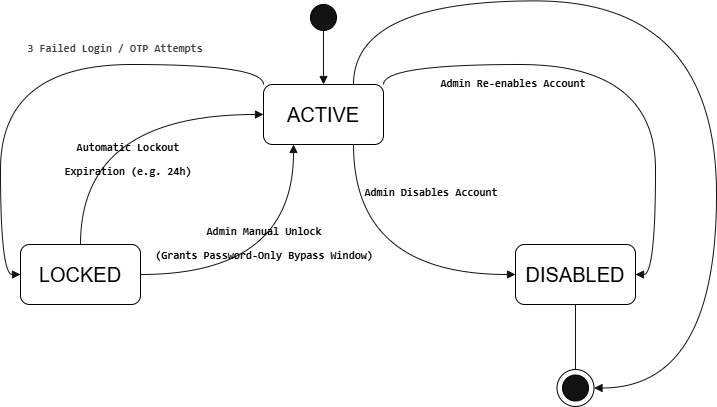
\includegraphics[width=1.1\textwidth]{images/out/diagrams/state/state_locked.png}}
    \caption{State Diagram -- Manage locked accounts}
    \label{fig:state_manage_locked}
\end{figure}

\newpage
\subsection{Sequence Diagram -- Use Case ``Manage profile''}
The diagram below illustrates the dynamic interactions for the ``Manage profile'' use case:

\begin{figure}[H]
    \centering
    \makebox[\textwidth][c]{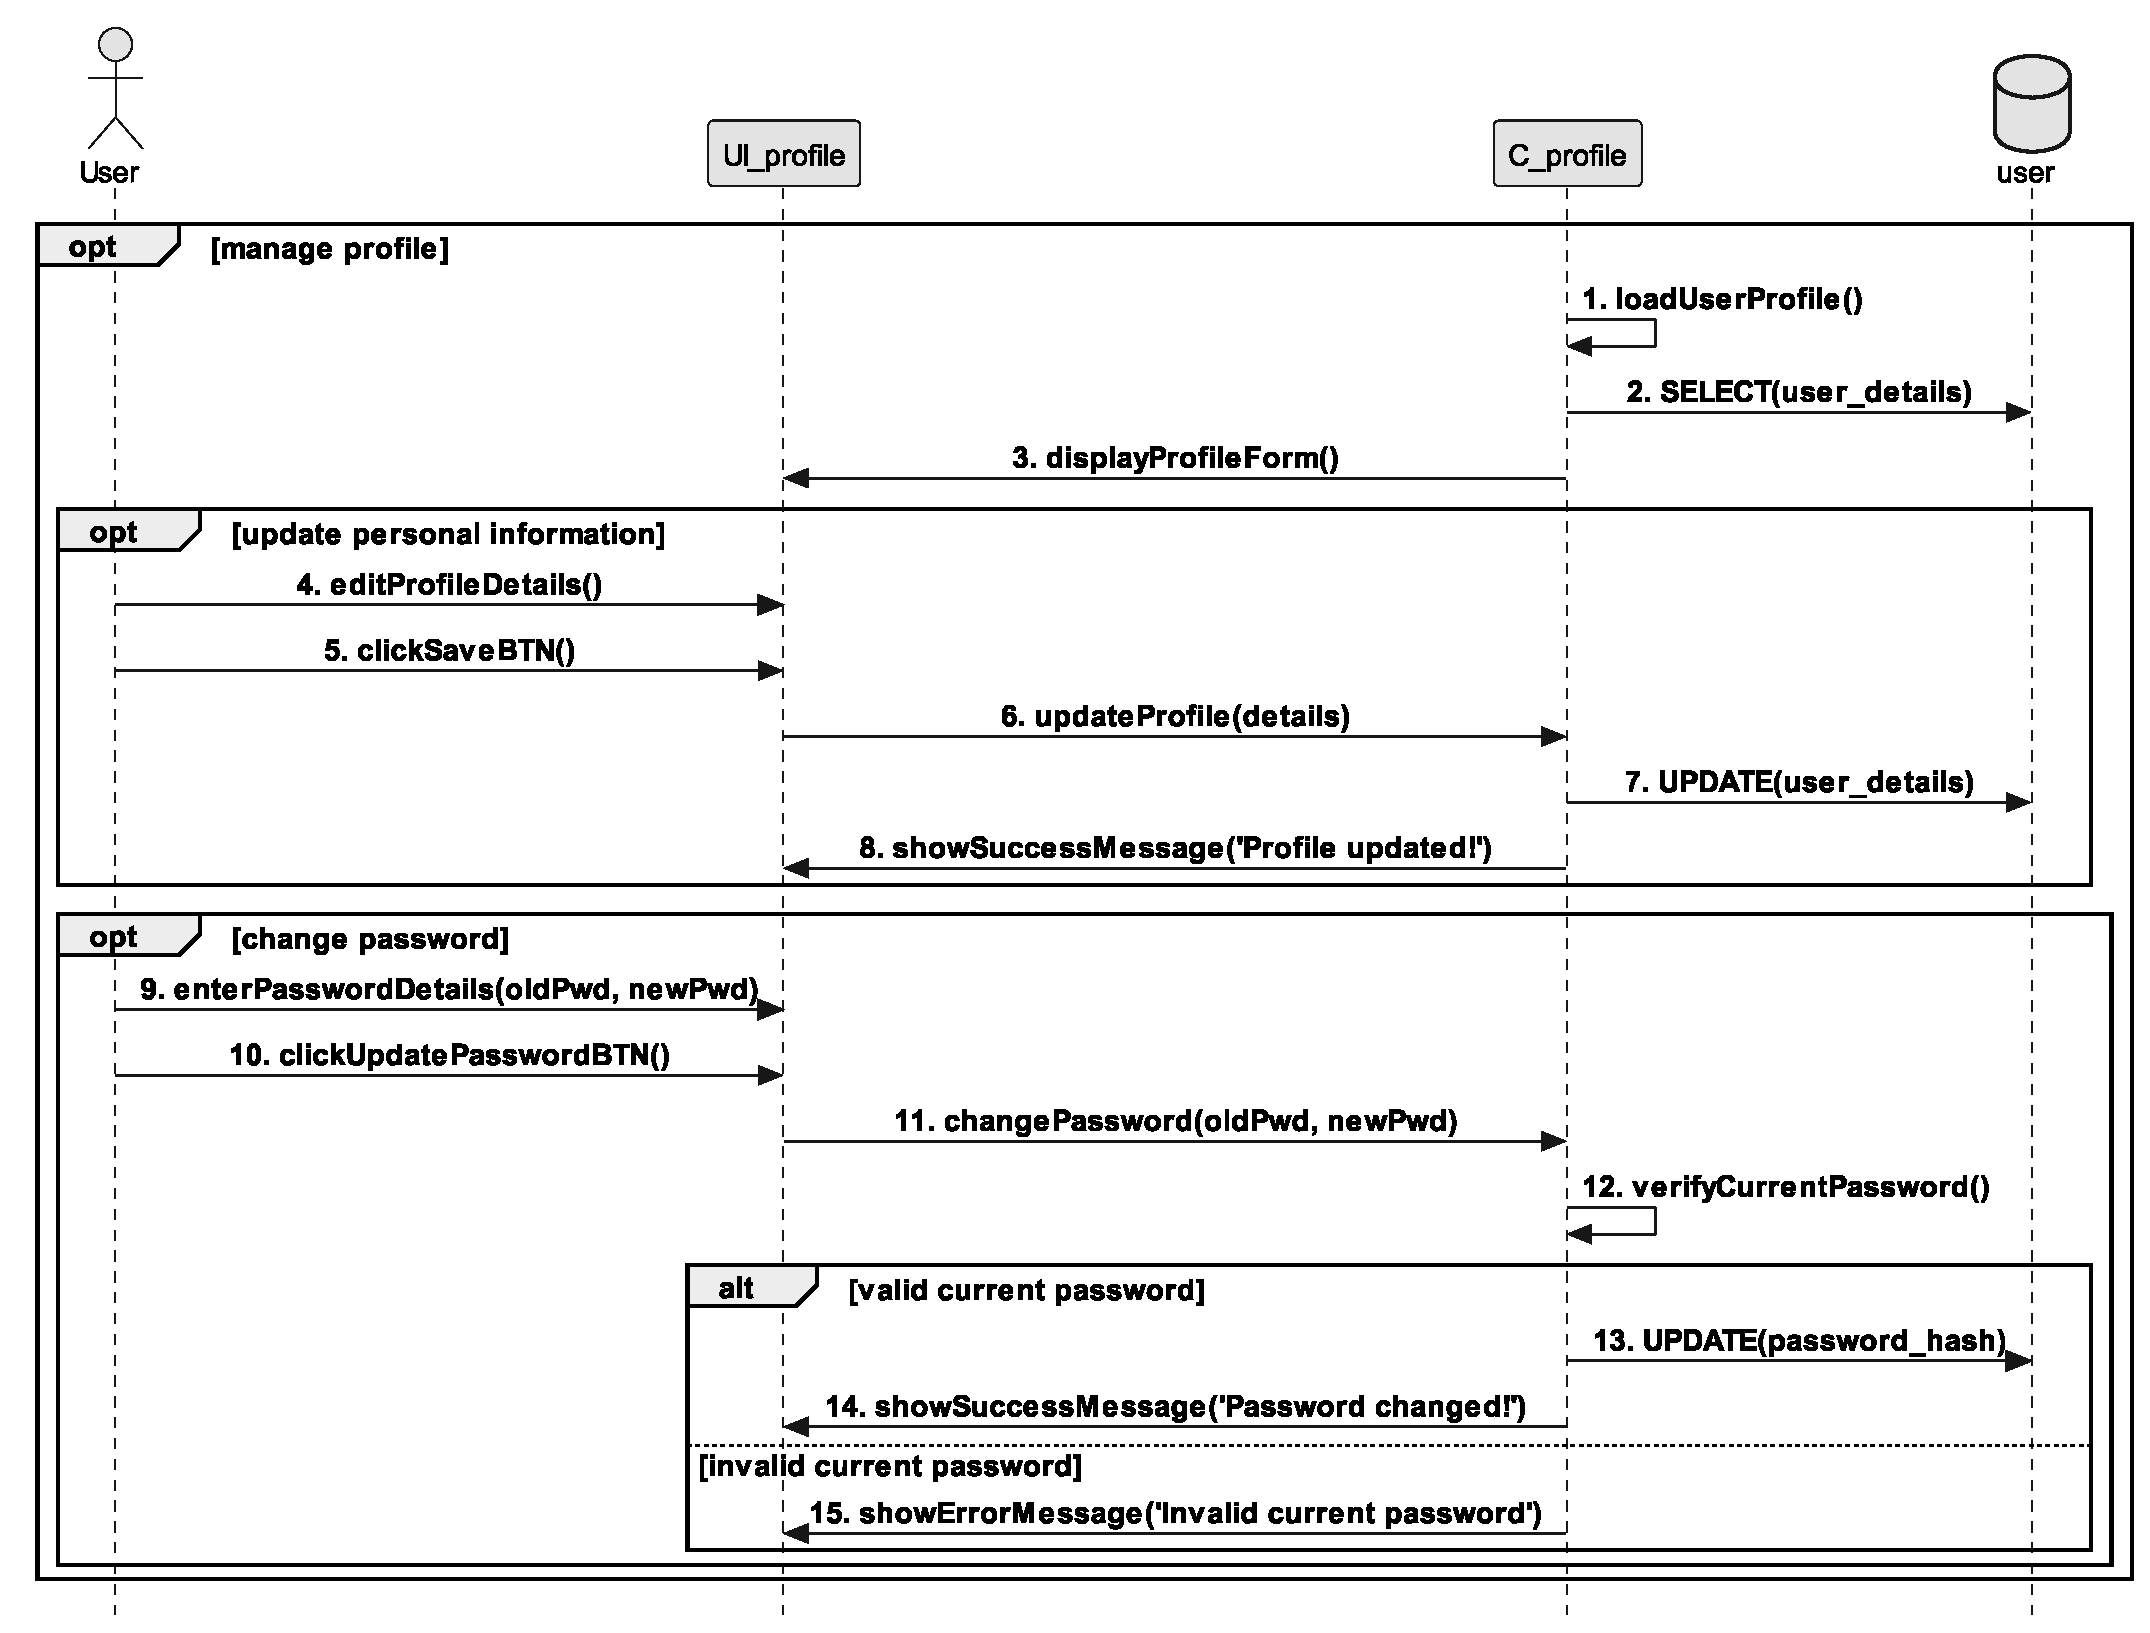
\includegraphics[width=1.2\textwidth]{images/out/diagrams/seq/manage_profile/manage_profile.eps}}
    \caption{Sequence Diagram -- Manage profile}
    \label{fig:seq_manage_profile}
\end{figure}

\newpage
\section{Sprint 1 Implementation}
This section presents the user interface implementations developed during Sprint 1.

\subsection{Company Contact Portal \& Surveys}
Figure \ref{fig:ui_my_surveys} displays the ``My Surveys'' interface where company contacts can consult active survey assignments, download template reference documents, and navigate to the online questionnaire.

\begin{figure}[H]
    \centering
    \makebox[\textwidth][c]{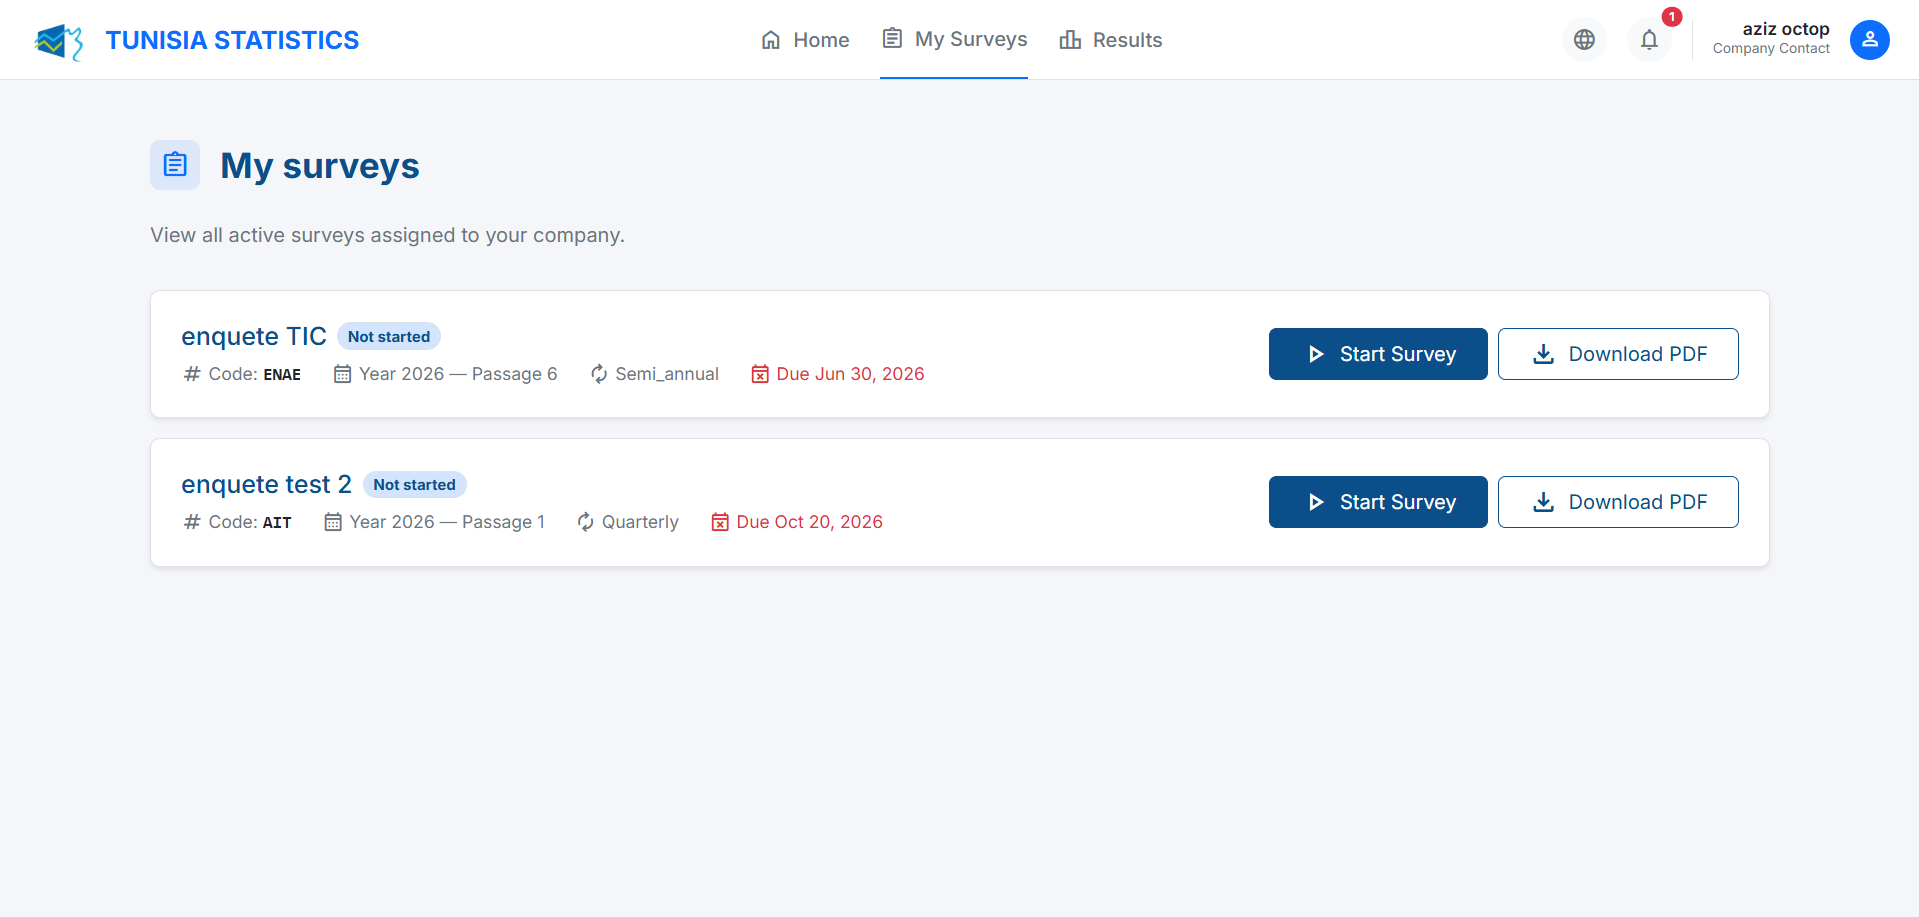
\includegraphics[width=0.9\textwidth]{images/screenshots/sprint1/my_surveys_page.png}}
    \caption{My Surveys Interface}
    \label{fig:ui_my_surveys}
\end{figure}


Figure \ref{fig:ui_overview_contact} shows the company contact portal overview dashboard presenting survey progress summary cards and quick shortcuts.

\begin{figure}[H]
    \centering
    \makebox[\textwidth][c]{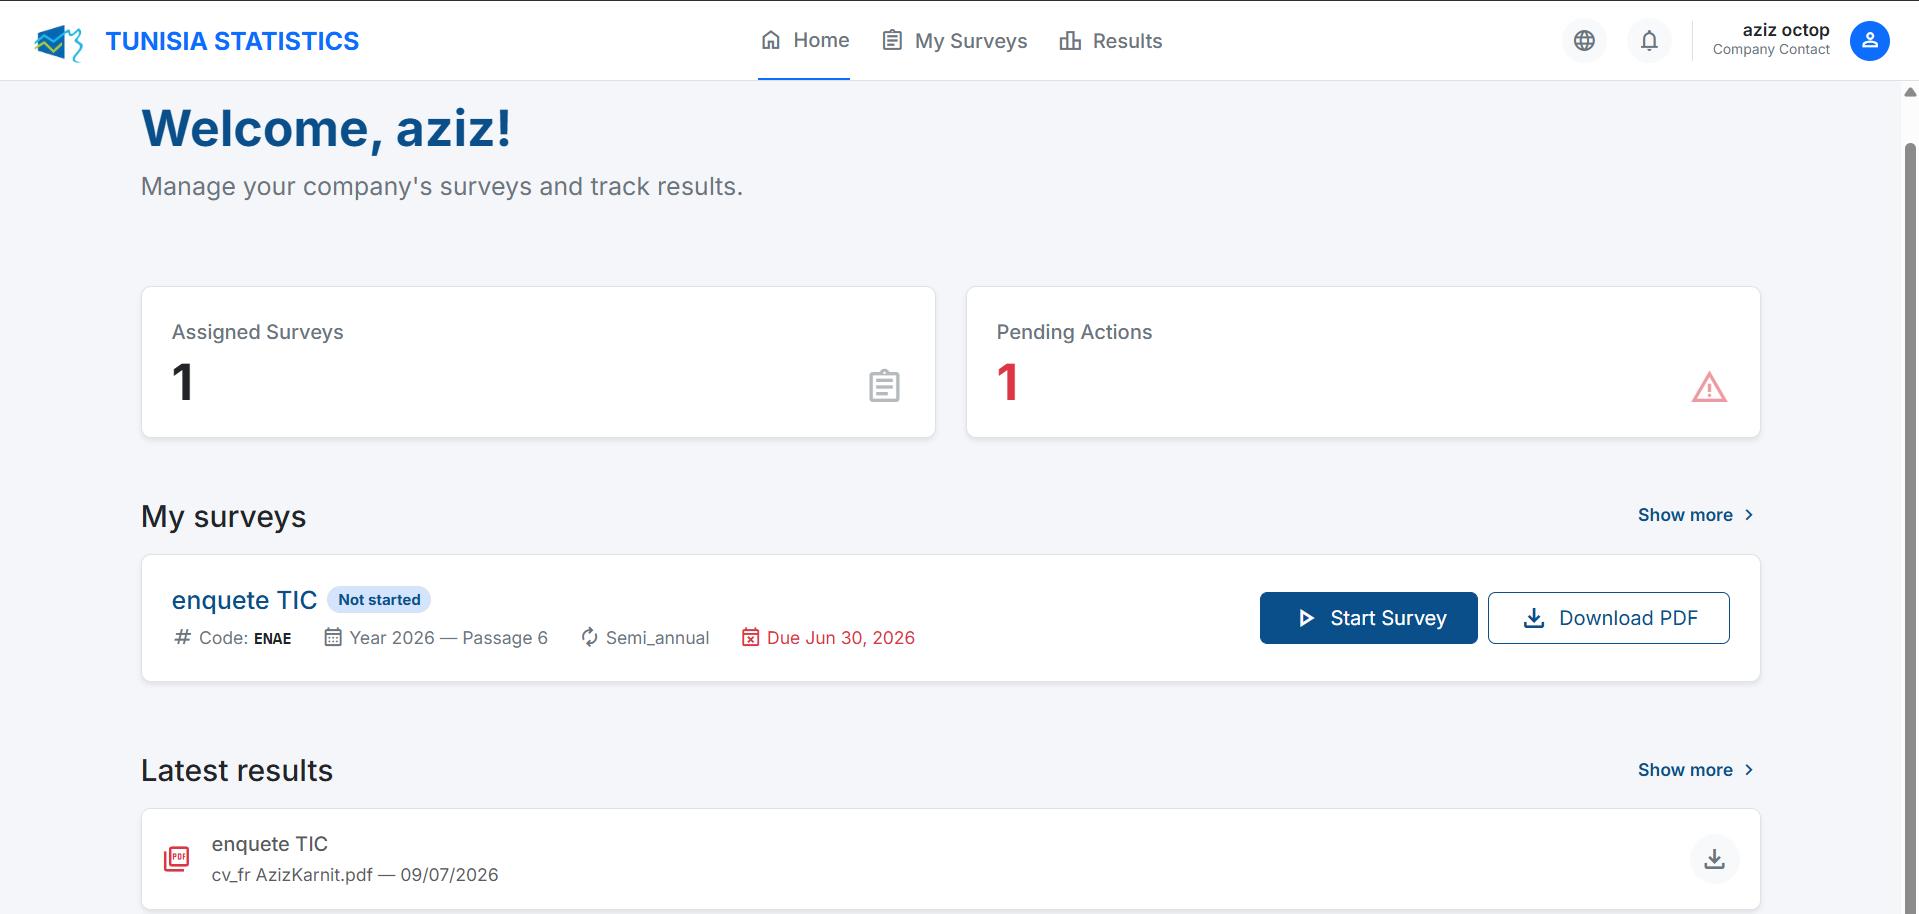
\includegraphics[width=0.9\textwidth]{images/screenshots/sprint1/overview_page_contact.png}}
    \caption{Company Contact Overview Dashboard}
    \label{fig:ui_overview_contact}
\end{figure}

Figure \ref{fig:ui_email_notification} shows the automated email notification received by company contacts upon being assigned to a survey passage.

\begin{figure}[H]
    \centering
    \makebox[\textwidth][c]{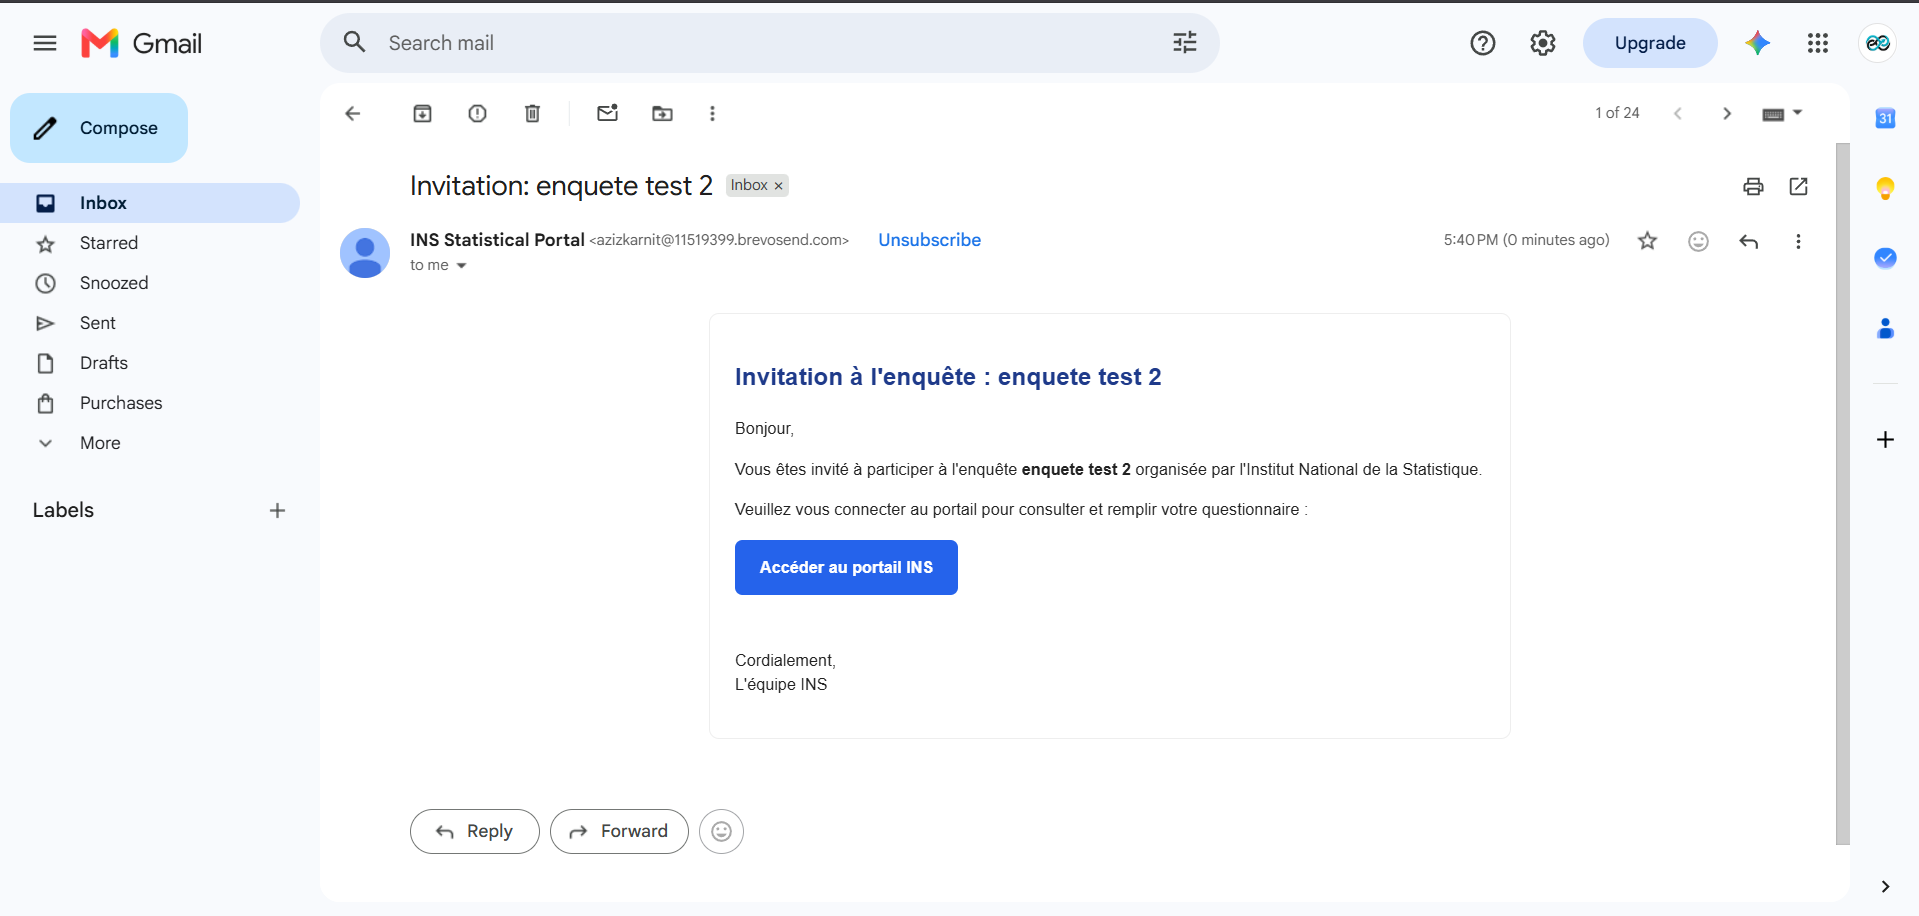
\includegraphics[width=0.9\textwidth]{images/screenshots/sprint1/email_notification_survey.png}}
    \caption{Survey Assignment Email Notification}
    \label{fig:ui_email_notification}
\end{figure}


\subsection{Consult Assigned Results Interface}
Figure \ref{fig:ui_consult_results} presents the survey reports and results interface allowing contacts to view past survey submissions and download published reports.

\begin{figure}[H]
    \centering
    \makebox[\textwidth][c]{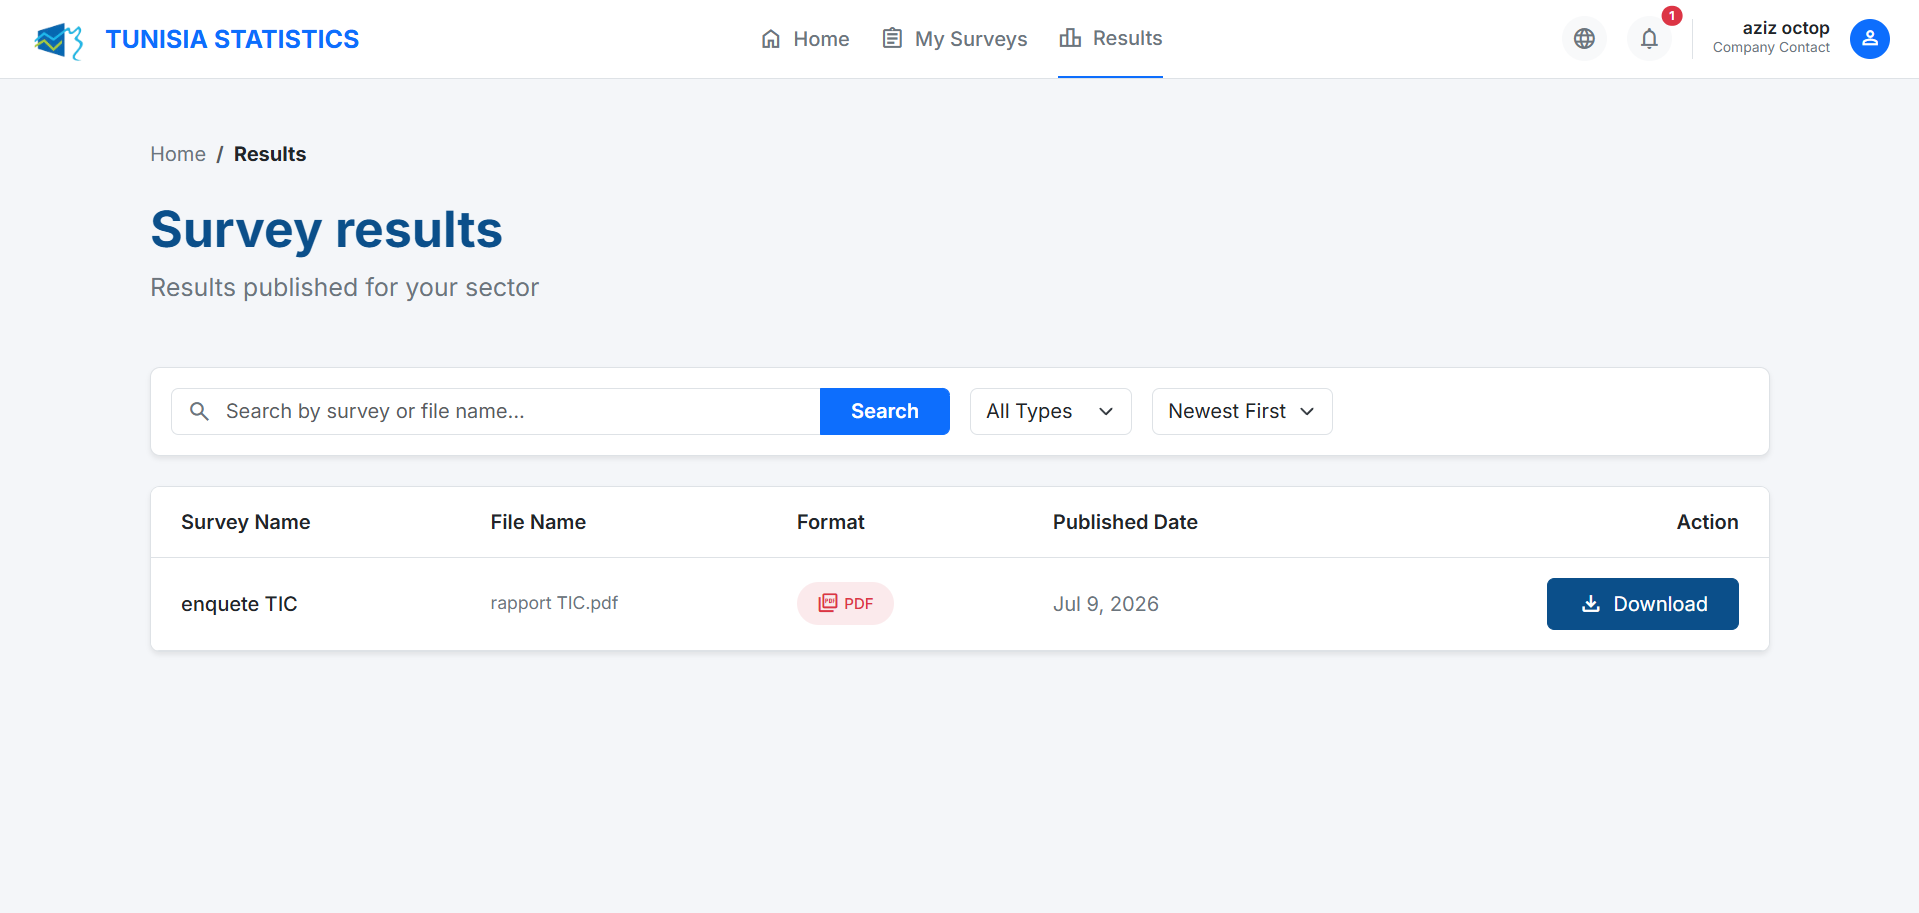
\includegraphics[width=0.9\textwidth]{images/screenshots/sprint1/rapports_page.png}}
    \caption{Consult Assigned Results \& Reports Interface}
    \label{fig:ui_consult_results}
\end{figure}

\newpage
\subsection{Manage System Settings Interface}
Figure \ref{fig:ui_manage_settings} shows the administrative system settings page for configuring global security parameters (2FA expiration, lockout duration, max attempts), default language, and email service providers.

\begin{figure}[H]
    \centering
    \makebox[\textwidth][c]{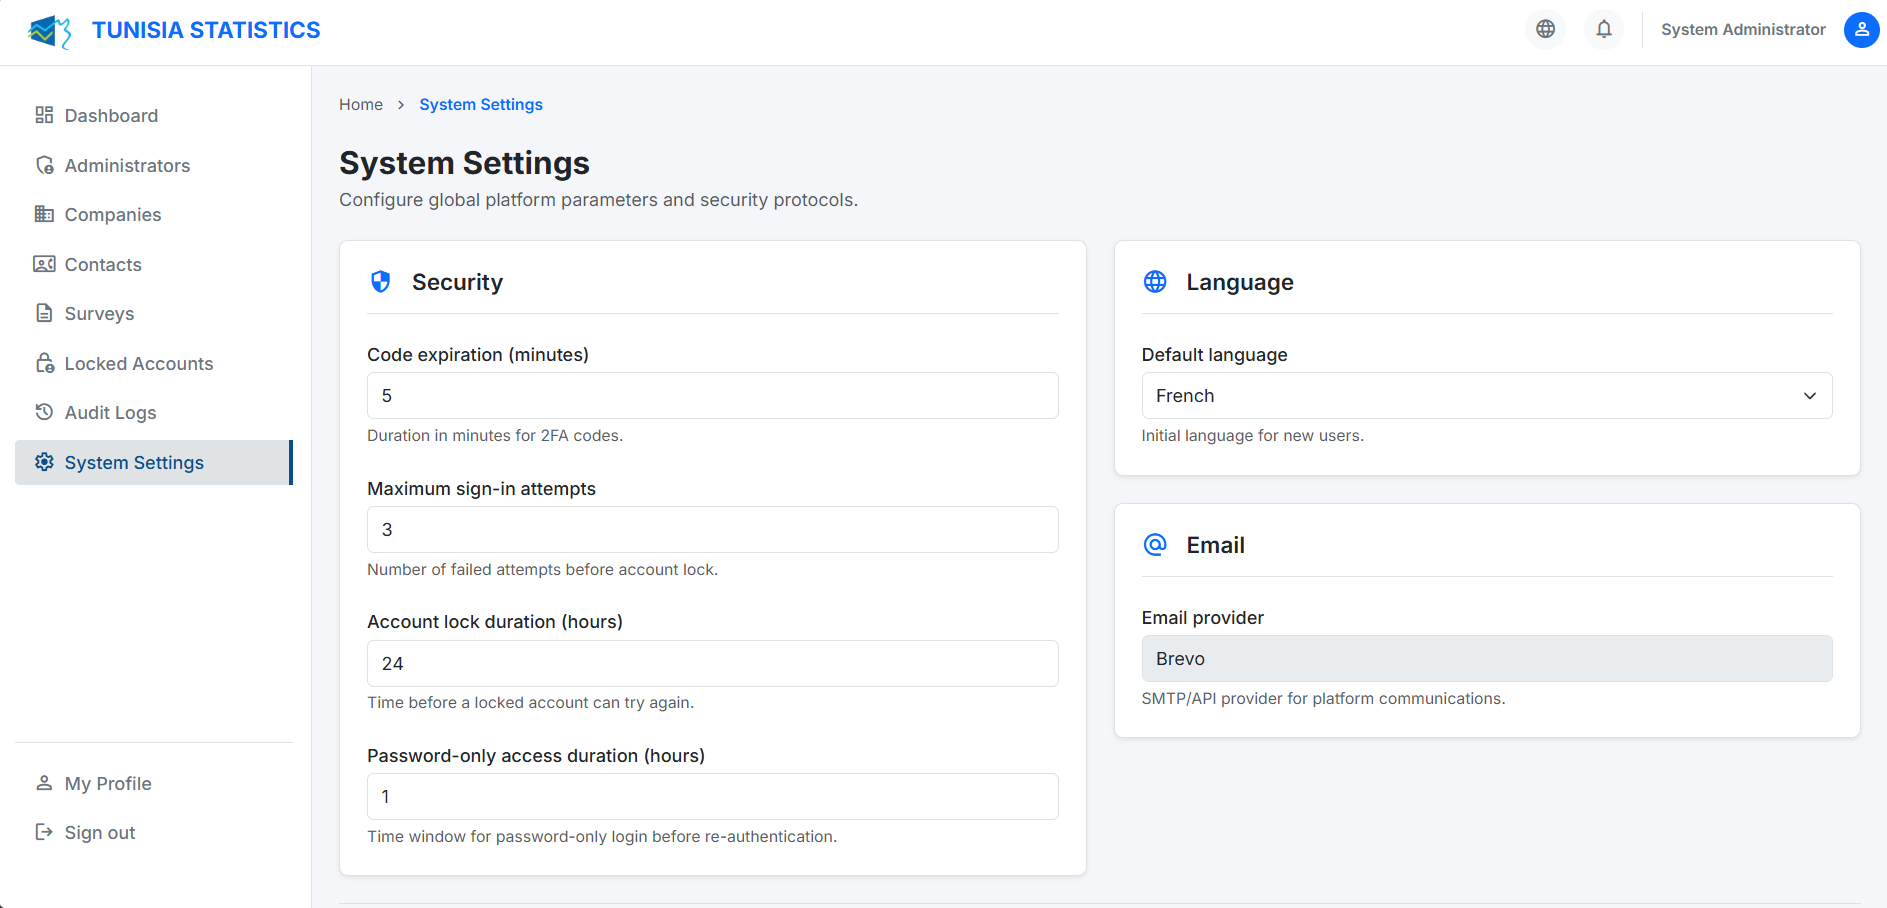
\includegraphics[width=0.9\textwidth]{images/screenshots/sprint1/system_settings_page.png}}
    \caption{System Settings Configuration Interface}
    \label{fig:ui_manage_settings}
\end{figure}

\subsection{Manage Locked Accounts \& Security Monitoring}
Figure \ref{fig:ui_manage_locked} displays the security monitoring table listing user accounts suspended due to repeated failed authentication attempts, allowing administrators to restore access.

\begin{figure}[H]
    \centering
    \makebox[\textwidth][c]{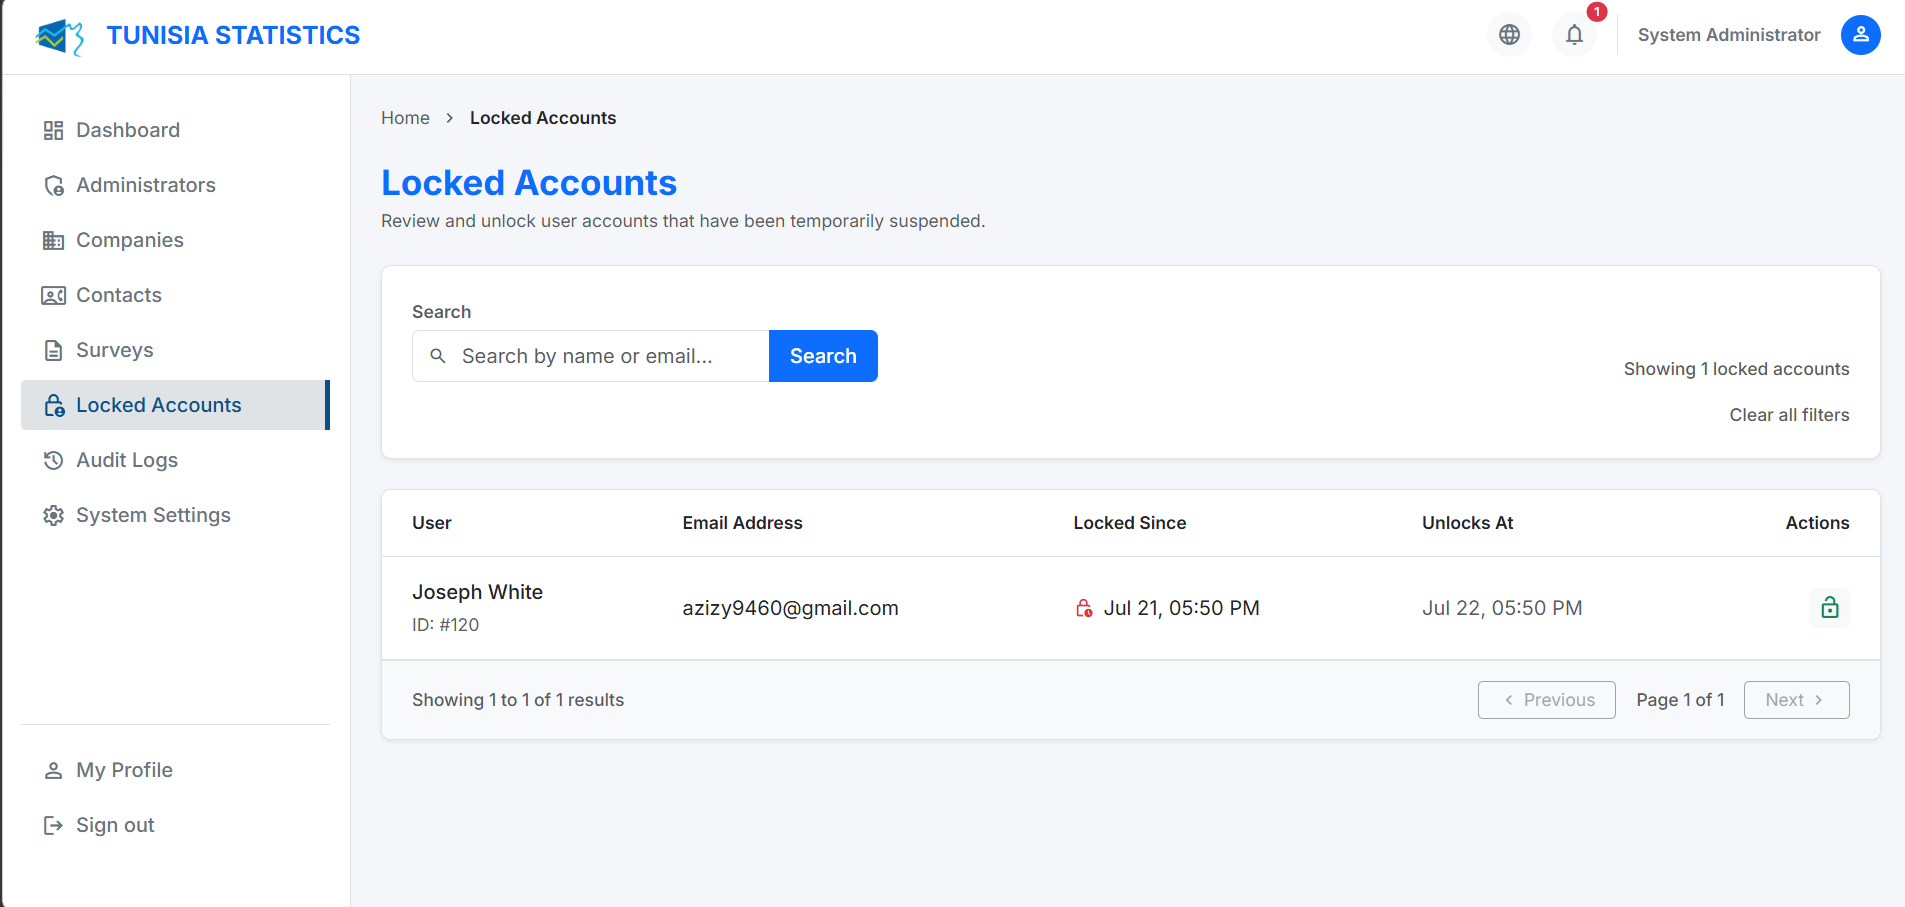
\includegraphics[width=1\textwidth]{images/screenshots/sprint1/locked_accounts_page.png}}
    \caption{Locked Accounts Management Interface}
    \label{fig:ui_manage_locked}
\end{figure}

Figure \ref{fig:ui_uncorrect_otp} shows the inline error feedback during two-factor authentication when an incorrect OTP is supplied.

\begin{figure}[H]
    \centering
    \makebox[\textwidth][c]{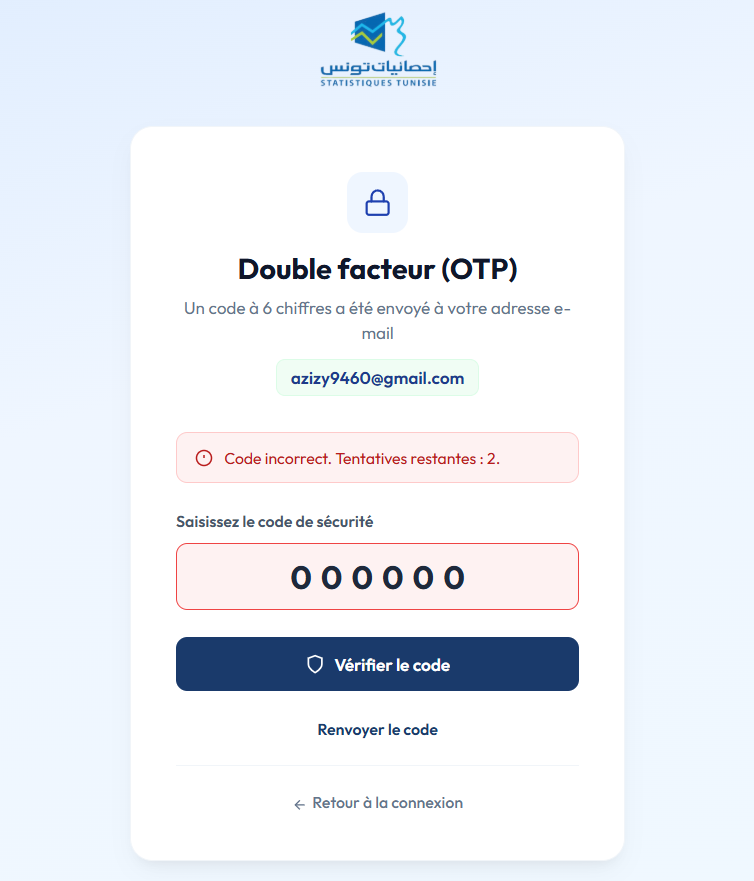
\includegraphics[width=0.5\textwidth]{images/screenshots/sprint1/uncorrect_OTP.png}}
    \caption{Incorrect OTP Validation Error}
    \label{fig:ui_uncorrect_otp}
\end{figure}

Figure \ref{fig:ui_locked_notification} illustrates the security notification banner informing the user when their account is locked due to security policy enforcement.

\begin{figure}[H]
    \centering
    \makebox[\textwidth][c]{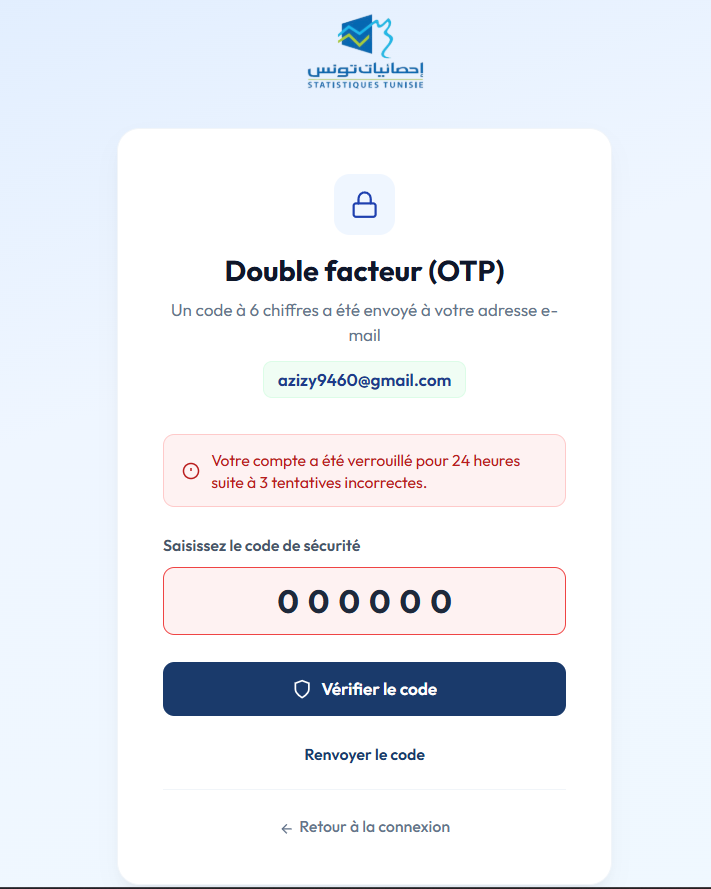
\includegraphics[width=0.4\textwidth]{images/screenshots/sprint1/locked_account_notification.png}}
    \caption{Account Lockout Security Warning}
    \label{fig:ui_locked_notification}
\end{figure}

\newpage
\subsection{Manage Profile Interface}
Figure \ref{fig:ui_profile_admin} shows the user profile management interface for administrators, enabling personal information updates and password changes.

\begin{figure}[H]
    \centering
    \makebox[\textwidth][c]{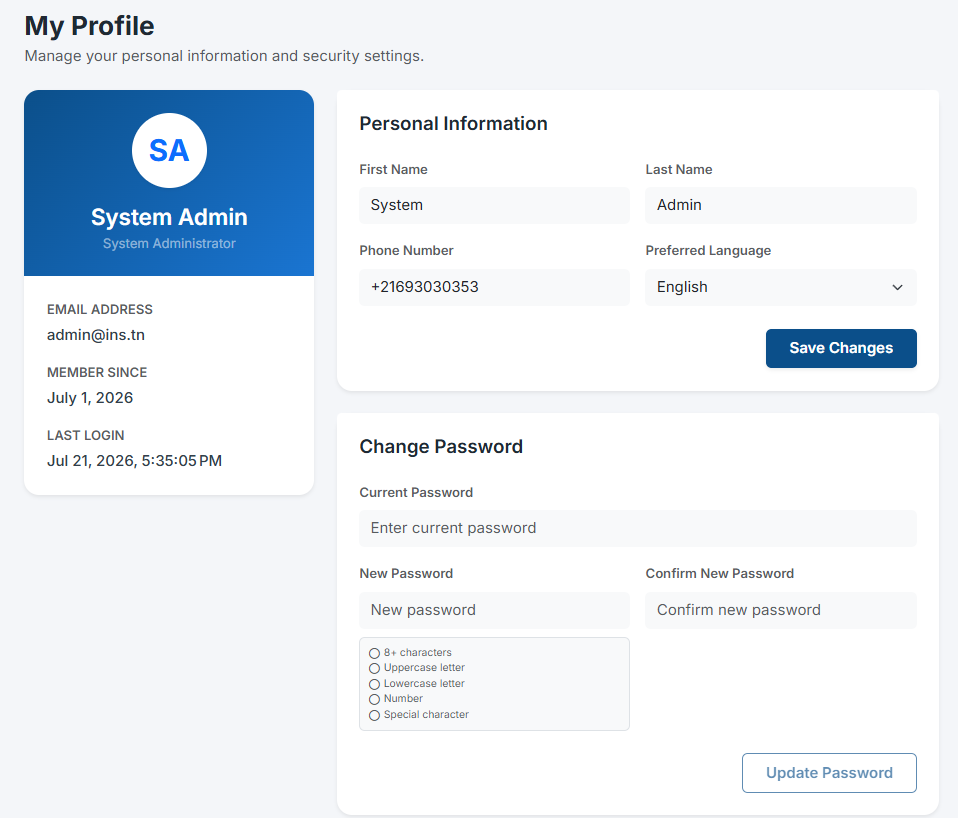
\includegraphics[width=1\textwidth]{images/screenshots/sprint1/profile_page_admins.png}}
    \caption{Admin Profile Management Interface}
    \label{fig:ui_profile_admin}
\end{figure}

\newpage
Figure \ref{fig:ui_profile_contact} illustrates the profile interface for company contacts.

\begin{figure}[H]
    \centering
    \makebox[\textwidth][c]{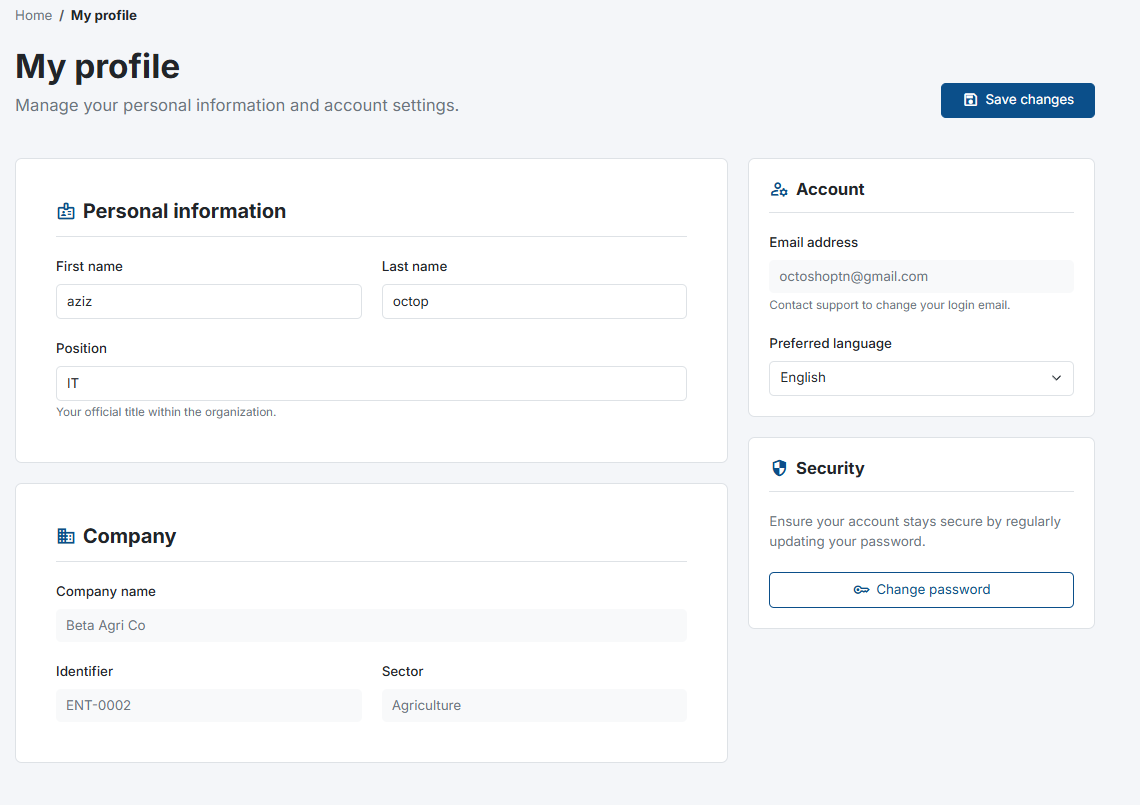
\includegraphics[width=1\textwidth]{images/screenshots/sprint1/profile_page_contacts.png}}
    \caption{Contact Profile Management Interface}
    \label{fig:ui_profile_contact}
\end{figure}

\section{UUID Token Architecture \& Security Analysis}
A key technical innovation implemented in Sprint 1 is the passwordless UUID token access system for external company respondents. Forcing external enterprise representatives to maintain traditional credentials creates account management friction and reduces statistical response rates.

To solve this, the platform generates a Universally Unique Identifier (UUID v4) for each \texttt{(contact\_id, passage\_id)} assignment pair. The token is mapped in the \texttt{questionnaire\_tokens} database table with a strict \texttt{UniqueConstraint("contact\_id", "passage\_id")}, ensuring one active token per respondent per survey passage.

When a company contact clicks their survey invitation link, the request is directed to the external questionnaire application with the UUID embedded as a parameter (\texttt{?token=uuid}). The external application executes a server-to-server REST call to the PFA backend endpoint \texttt{POST /api/v1/ext/resolve}, protected by a shared API key (\texttt{X-API-Key}). The endpoint validates the token, enforces passage closing date restrictions, initializes collection tracking, and returns questionnaire data without exposing company PII.

Listing \ref{lst:uuid_model} shows the database model, and Listing \ref{lst:uuid_resolve} shows the token resolution endpoint.

\begin{lstlisting}[language=Python, caption={Questionnaire Token Database Model (\texttt{app/models/questionnaire\_token.py})}, label={lst:uuid_model}]
class QuestionnaireToken(Base):
    __tablename__ = "questionnaire_tokens"
    __table_args__ = (
        UniqueConstraint(
            "contact_id", "passage_id", 
            name="uq_contact_passage_token"
        ),
    )
    id: Mapped[int] = mapped_column(
        Integer, primary_key=True, index=True
    )
    token: Mapped[str] = mapped_column(
        String(50), unique=True, index=True
    )
    contact_id: Mapped[int] = mapped_column(
        Integer, ForeignKey("contacts.id")
    )
    company_id: Mapped[int] = mapped_column(
        Integer, ForeignKey("companies.id")
    )
    passage_id: Mapped[int] = mapped_column(
        Integer, ForeignKey("survey_passages.id")
    )
\end{lstlisting}

\begin{lstlisting}[language=Python, caption={External Token Resolution Endpoint (\texttt{app/api/v1/external\_integration.py})}, label={lst:uuid_resolve}]
@router.post("/resolve", response_model=ResolveTokenResponse)
def resolve_uuid_token(
    payload: ResolveTokenRequest,
    db: Session = Depends(get_db),
    api_key: str = Depends(verify_api_key)
):
    token_obj = db.query(QuestionnaireToken).filter(
        QuestionnaireToken.token == payload.uuid
    ).first()
    if not token_obj:
        raise HTTPException(
            status_code=404, 
            detail="UUID token not found or invalid"
        )
    passage = token_obj.passage
    if passage.closing_date < datetime.datetime.now():
        raise HTTPException(
            status_code=400, 
            detail="The survey passage has closed."
        )
    return ResolveTokenResponse(...)
\end{lstlisting}

\section{Sprint 1 Conclusion}
This chapter detailed the development of Sprint 1, which successfully delivered the company portal capabilities allowing external contacts to consult surveys, download templates, and upload their submissions. Additionally, secondary administrative tools such as system settings configuration, locked account management, and the passwordless UUID token integration were completed. The next chapter details Sprint 2, which focuses on the notification engine, systemic auditing, and overall system testing.

\newpage
\chapter{Sprint 2 -- Notification Engine \& Systemic Auditing}

\section{Introduction}
This section details the development of Sprint 2, which focuses on the notification engine, comprehensive systemic auditing, and platform validation. It presents the sprint backlog, the detailed refinement of each user story, class diagram updates, dynamic behavior models, user interface implementations, and system testing.

\section{Sprint 2 Backlog}
The Sprint 2 backlog encompasses the functional requirements for user notification management and security audit logging.

\begin{table}[H]
\centering
\caption{Sprint 2 Backlog}
\vspace{0.3cm}
\renewcommand{\arraystretch}{1.3}
\begin{tabular}{|c|p{11cm}|c|}
\hline
\textbf{ID} & \textbf{User Story} & \textbf{Priority} \\ \hline
US11 & As a user, I want to Consult notifications to view and manage system alerts and activity updates. & High \\ \hline
US12 & As a System Administrator or Survey Manager, I want to Consult audit logs to monitor system security and track user actions. & High \\ \hline
\end{tabular}
\end{table}

\section{Sprint 2 Refinement}
In this section, we refine the functional details and textual specifications for the use cases of Sprint 2.

\newpage
\subsection{Refinement of the Use Case ``Consult notifications''}
The diagram below illustrates the refinement of the ``Consult notifications'' use case and its interactions with system actors:

\begin{figure}[H]
    \centering
    \makebox[\textwidth][c]{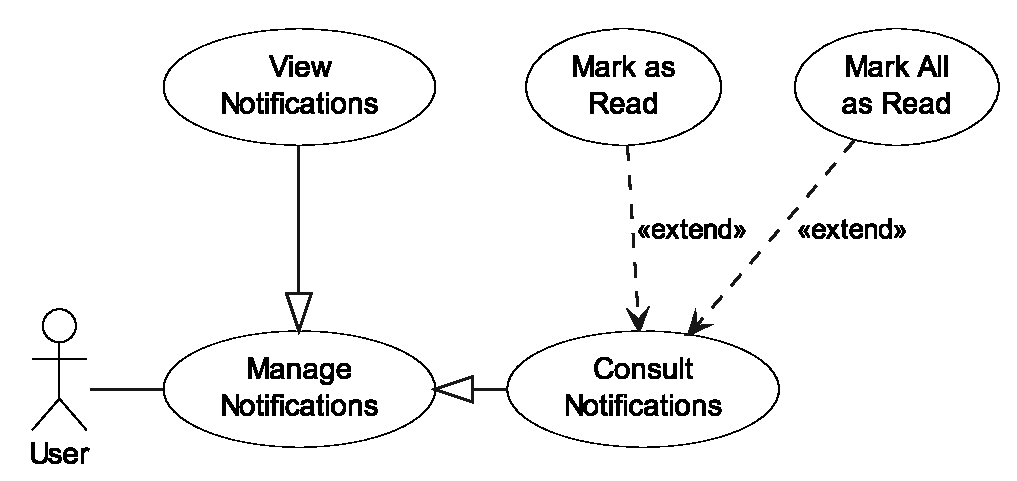
\includegraphics[width=0.85\textwidth]{images/out/diagrams/use_case/consult_notifications/consult_notifications.eps}}
    \caption{Use Case Diagram -- Consult notifications}
    \label{fig:uc_consult_notifications}
\end{figure}

Table \ref{tab:refinement_consult_notifications} presents the textual description of the ``Consult notifications'' use case:

\begin{table}[H]
\centering
\caption{Textual description -- Consult notifications}
\label{tab:refinement_consult_notifications}
\vspace{0.2cm}
\small
\renewcommand{\arraystretch}{1.15}
\begin{tabular}{|p{3.5cm}|p{12.0cm}|}
\hline
\textbf{Use Case} & Consult notifications \\ \hline
\textbf{Actor} & Any authenticated user \\ \hline
\textbf{Pre-condition} & The user is logged in to the platform. \\ \hline
\textbf{Post-condition} & The user views their notifications and can mark items as read. \\ \hline
\textbf{Main Scenario} & 
1. The user clicks on the notification bell icon in the top header. \newline
2. The system fetches and displays a dropdown list of recent unread notifications. \newline
3. The user selects ``View All Notifications'' to open the full notification center. \newline
4. The system lists all notifications categorized by date and severity. \newline
5. The user clicks ``Mark as Read'' on an item or ``Mark All as Read''. \newline
6. The system updates the read status in the database and updates the header badge counter. \\ \hline
\textbf{Alternative Scenarios} & 
$\bullet$ No notifications: The system displays a ``No new notifications'' placeholder. \\ \hline
\textbf{Exception} & Real-time connection drop; the system retries fetching notifications on the next polling interval. \\ \hline
\end{tabular}
\end{table}

\newpage
\subsection{Refinement of the Use Case ``Consult audit logs''}
The diagram below illustrates the refinement of the ``Consult audit logs'' use case and its interactions with system actors:

\begin{figure}[H]
    \centering
    \makebox[\textwidth][c]{\includegraphics[width=1.1\textwidth]{images/out/diagrams/use_case/audit_logs/audit_logs.eps}}
    \caption{Use Case Diagram -- Consult audit logs}
    \label{fig:uc_consult_audit}
\end{figure}

Table \ref{tab:refinement_consult_audit} presents the textual description of the ``Consult audit logs'' use case:

\begin{table}[H]
\centering
\caption{Textual description -- Consult audit logs}
\label{tab:refinement_consult_audit}
\vspace{0.2cm}
\small
\renewcommand{\arraystretch}{1.15}
\begin{tabular}{|p{3.5cm}|p{12.0cm}|}
\hline
\textbf{Use Case} & Consult audit logs \\ \hline
\textbf{Actor} & System Administrator, Survey Manager \\ \hline
\textbf{Pre-condition} & The user is logged in with administrative or managerial permissions. \\ \hline
\textbf{Post-condition} & Audit records are queried, filtered, and optionally exported. \\ \hline
\textbf{Main Scenario} & 
1. The administrator navigates to the ``Audit Logs'' section. \newline
2. The system loads the audit trail table displaying timestamp, actor, action type, target entity, and IP address. \newline
3. The administrator applies filters (e.g., date range, user, action type). \newline
4. The system updates the table view with matching audit events. \newline
5. (Optional) The administrator clicks ``Export Audit Log''. \newline
6. The system triggers a background task to generate an Excel/PDF export report. \\ \hline
\textbf{Alternative Scenarios} & 
$\bullet$ No matching logs: The system displays a ``No audit events found'' message. \\ \hline
\textbf{Exception} & Query timeout; the system displays an error and prompts for narrower date filtering. \\ \hline
\end{tabular}
\end{table}

\newpage
\section{Sprint 2 Conception}
In this section, we present the structural and dynamic models for Sprint 2.

\subsection{Class Diagram -- Sprint 2 Core Domain}
The class diagram below models the complete system architecture including the notification and audit entities:

\begin{figure}[H]
    \centering
    \makebox[\textwidth][c]{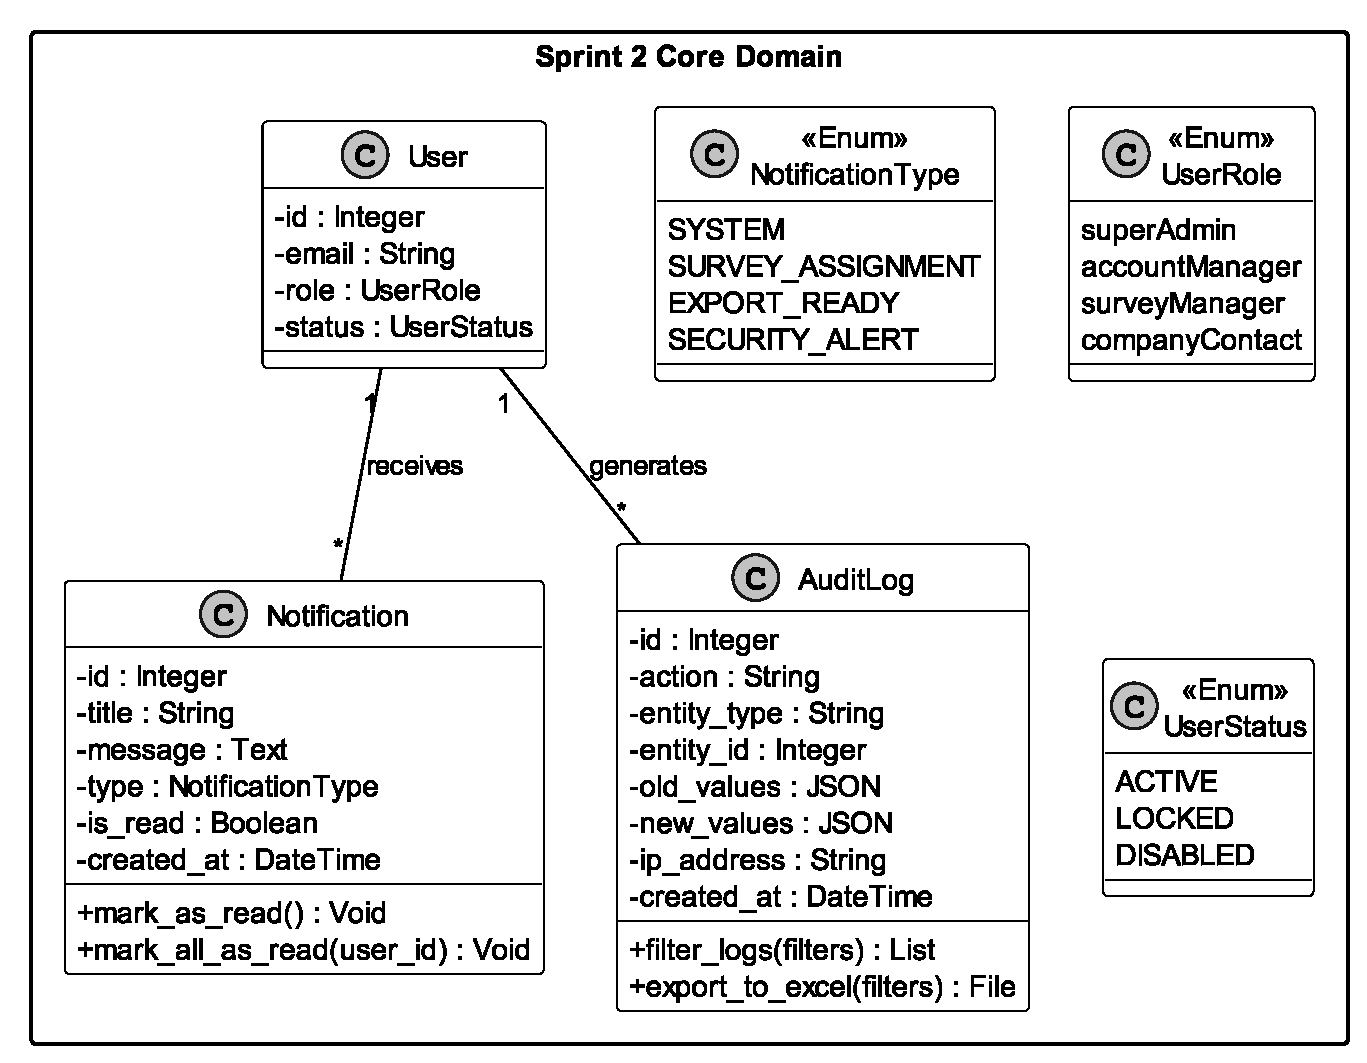
\includegraphics[width=1.1\textwidth]{images/out/diagrams/class/sprint2/sprint2.eps}}
    \caption{Sprint 2 Class Diagram}
    \label{fig:sprint2_class_diagram}
\end{figure}

The Sprint 2 class diagram (Figure \ref{fig:sprint2_class_diagram}) completes the platform data architecture by adding systemic monitoring and notification entities. The \texttt{AppNotification} class stores persistent user alerts linked to \texttt{User} via a foreign key, recording notification title, message body, read status, type, and contextual action URL. Systemic security auditing is supported by \texttt{AuditLog}, which captures system events with actor user ID, action type (LOGIN, CREATE, UPDATE, DELETE, EXPORT), entity target, timestamp, and client IP address. Furthermore, \texttt{ImportSession} and \texttt{CompanyImportStaging} model the staging workflow for bulk company file ingestion.

\subsection{Activity Diagram -- Use Case ``Consult notifications''}
The activity diagram below illustrates the multi-tier workflow and decision logic across system layers for real-time notification delivery and user interactions:

\begin{figure}[H]
    \centering
    \makebox[\textwidth][c]{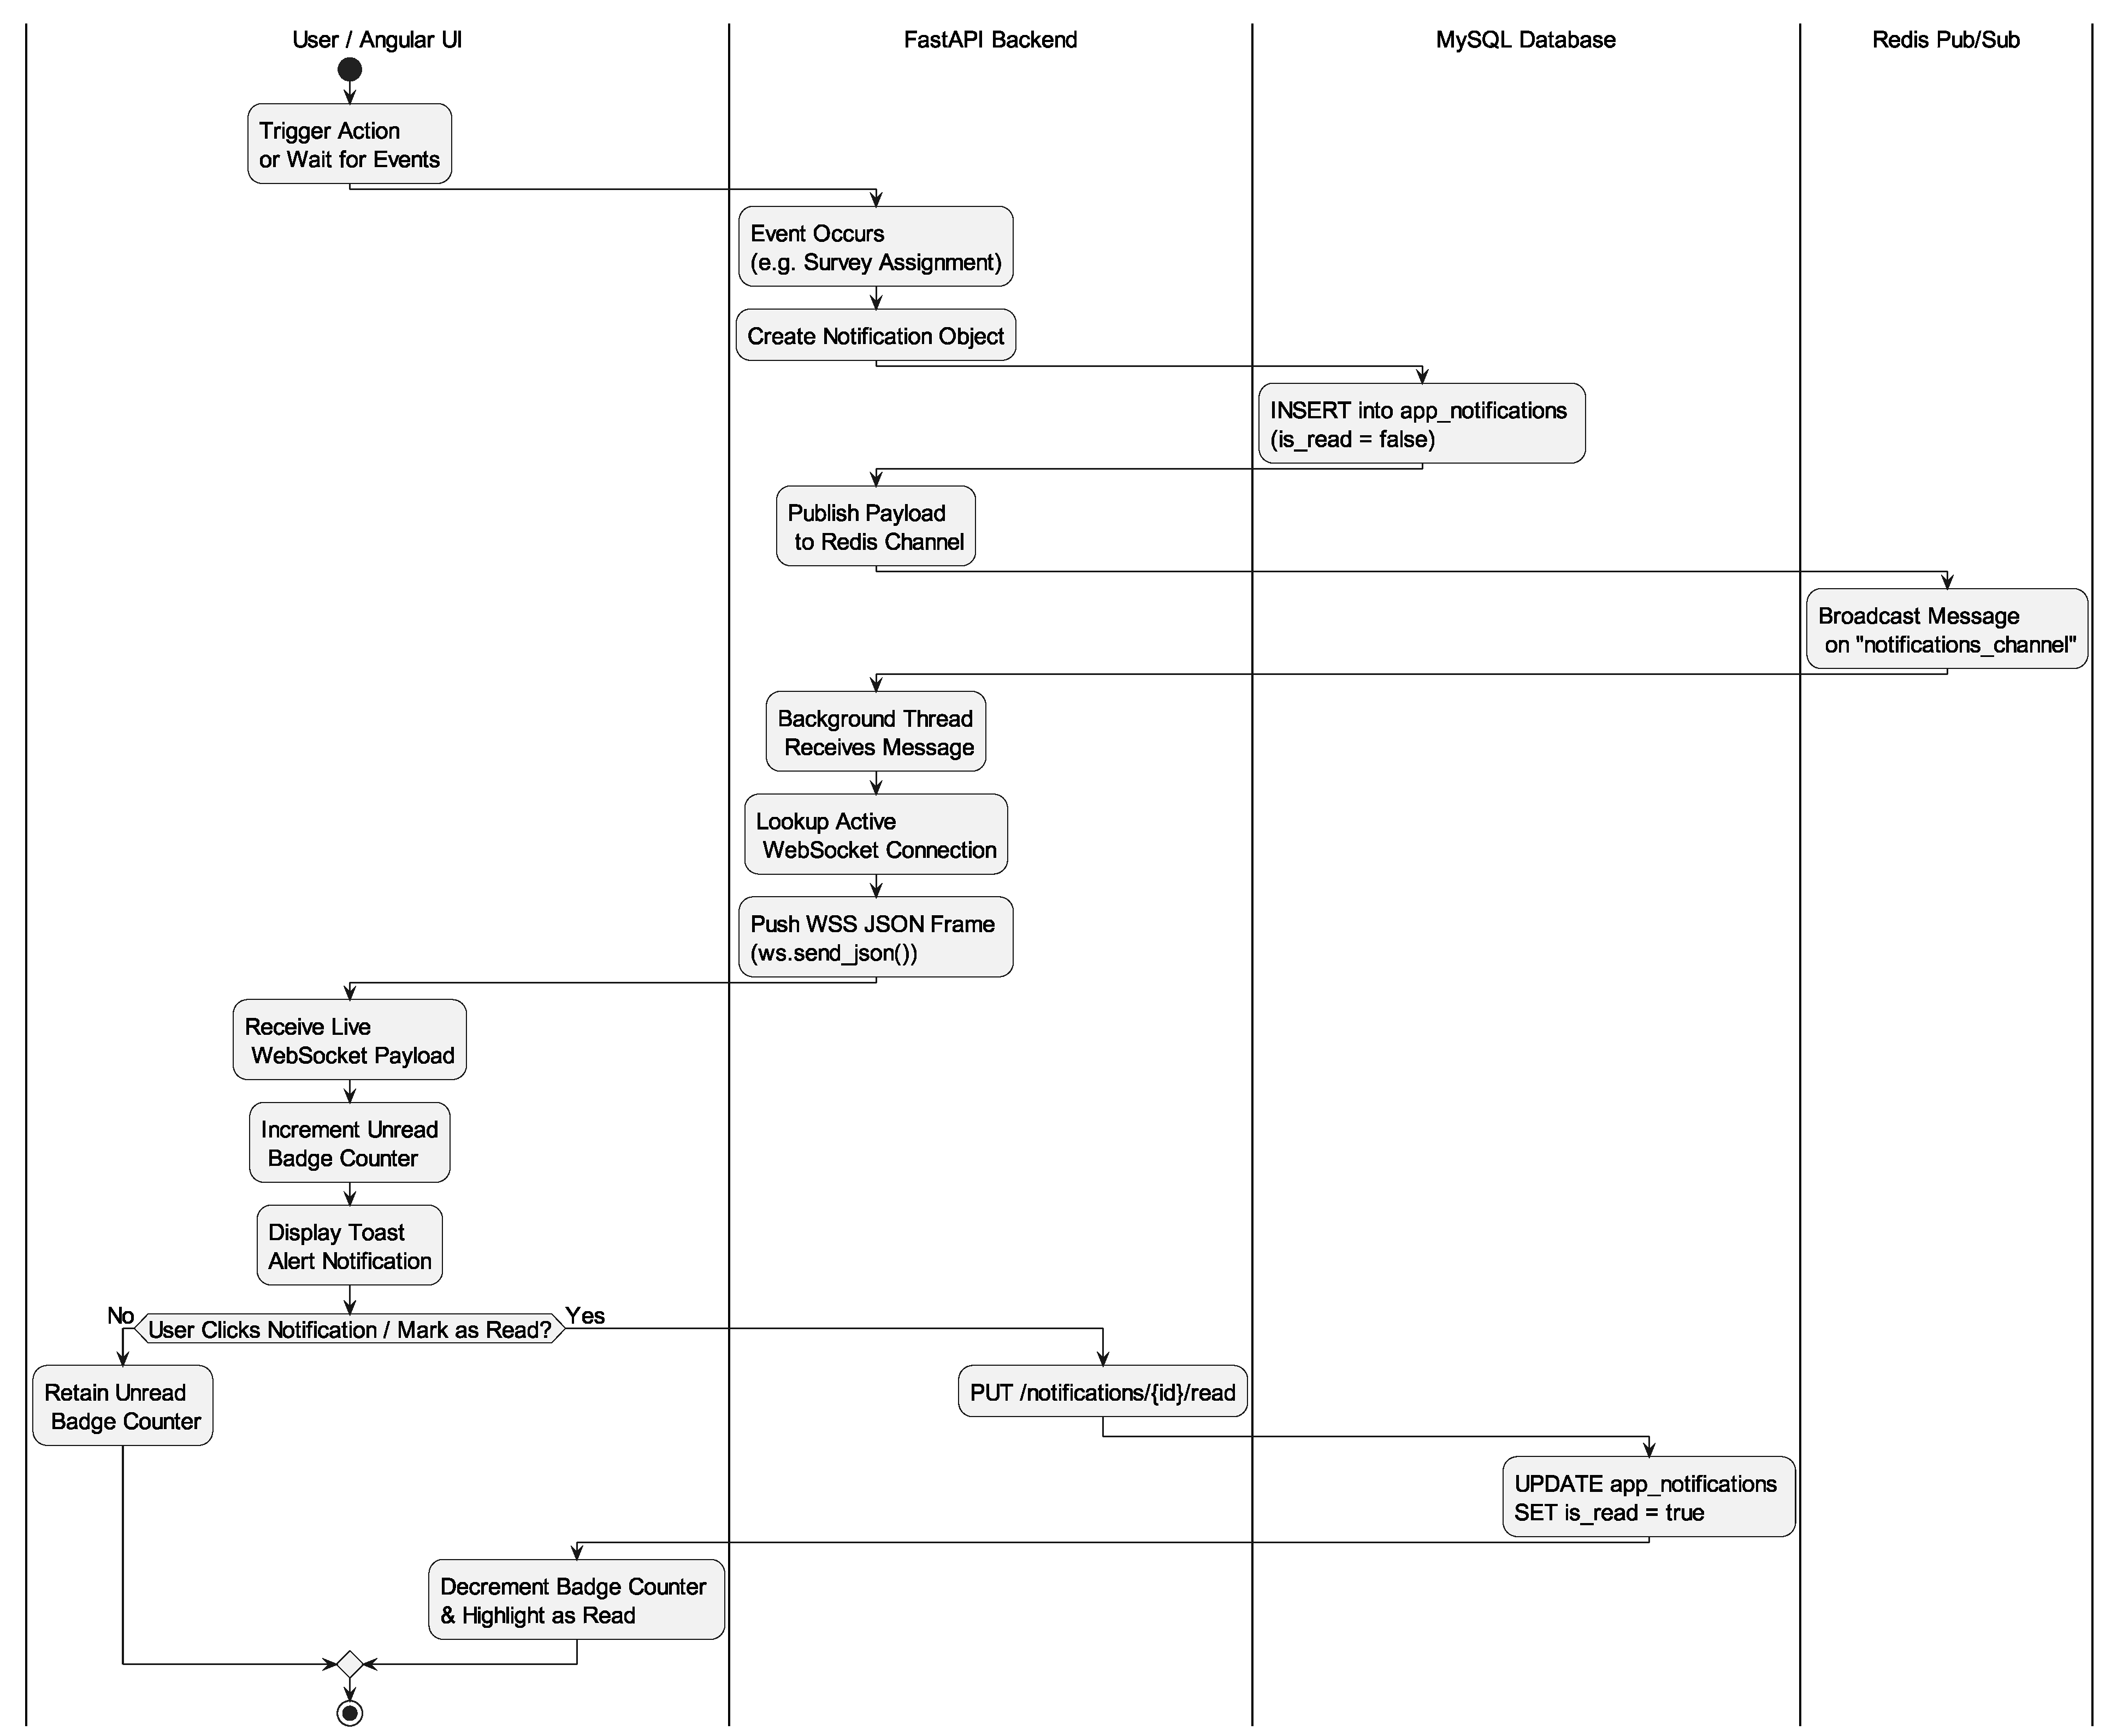
\includegraphics[width=0.8\textheight]{images/out/diagrams/activite/notif/notif.eps}}
    \caption{Activity Diagram -- Consult notifications}
    \label{fig:act_consult_notifications}
\end{figure}

\newpage
\subsection{State Diagram -- Notification Life Cycle}
The state diagram below models the transitions of a notification from creation and real-time delivery to user consultation and archival:

\begin{figure}[H]
    \centering
    \makebox[\textwidth][c]{\includegraphics[width=1.1\textwidth]{images/out/diagrams/state/notif/notif.eps}}
    \caption{State Diagram -- Notification Life Cycle}
    \label{fig:state_notification}
\end{figure}

\newpage
\subsection{Sequence Diagram -- Use Case ``Consult audit logs''}
The sequence diagram below details the step-by-step interactions between the System Administrator, Frontend UI, API Controller, Celery Worker, and Database during audit log consultation and asynchronous Excel export:

\begin{figure}[H]
    \centering
    \makebox[\textwidth][c]{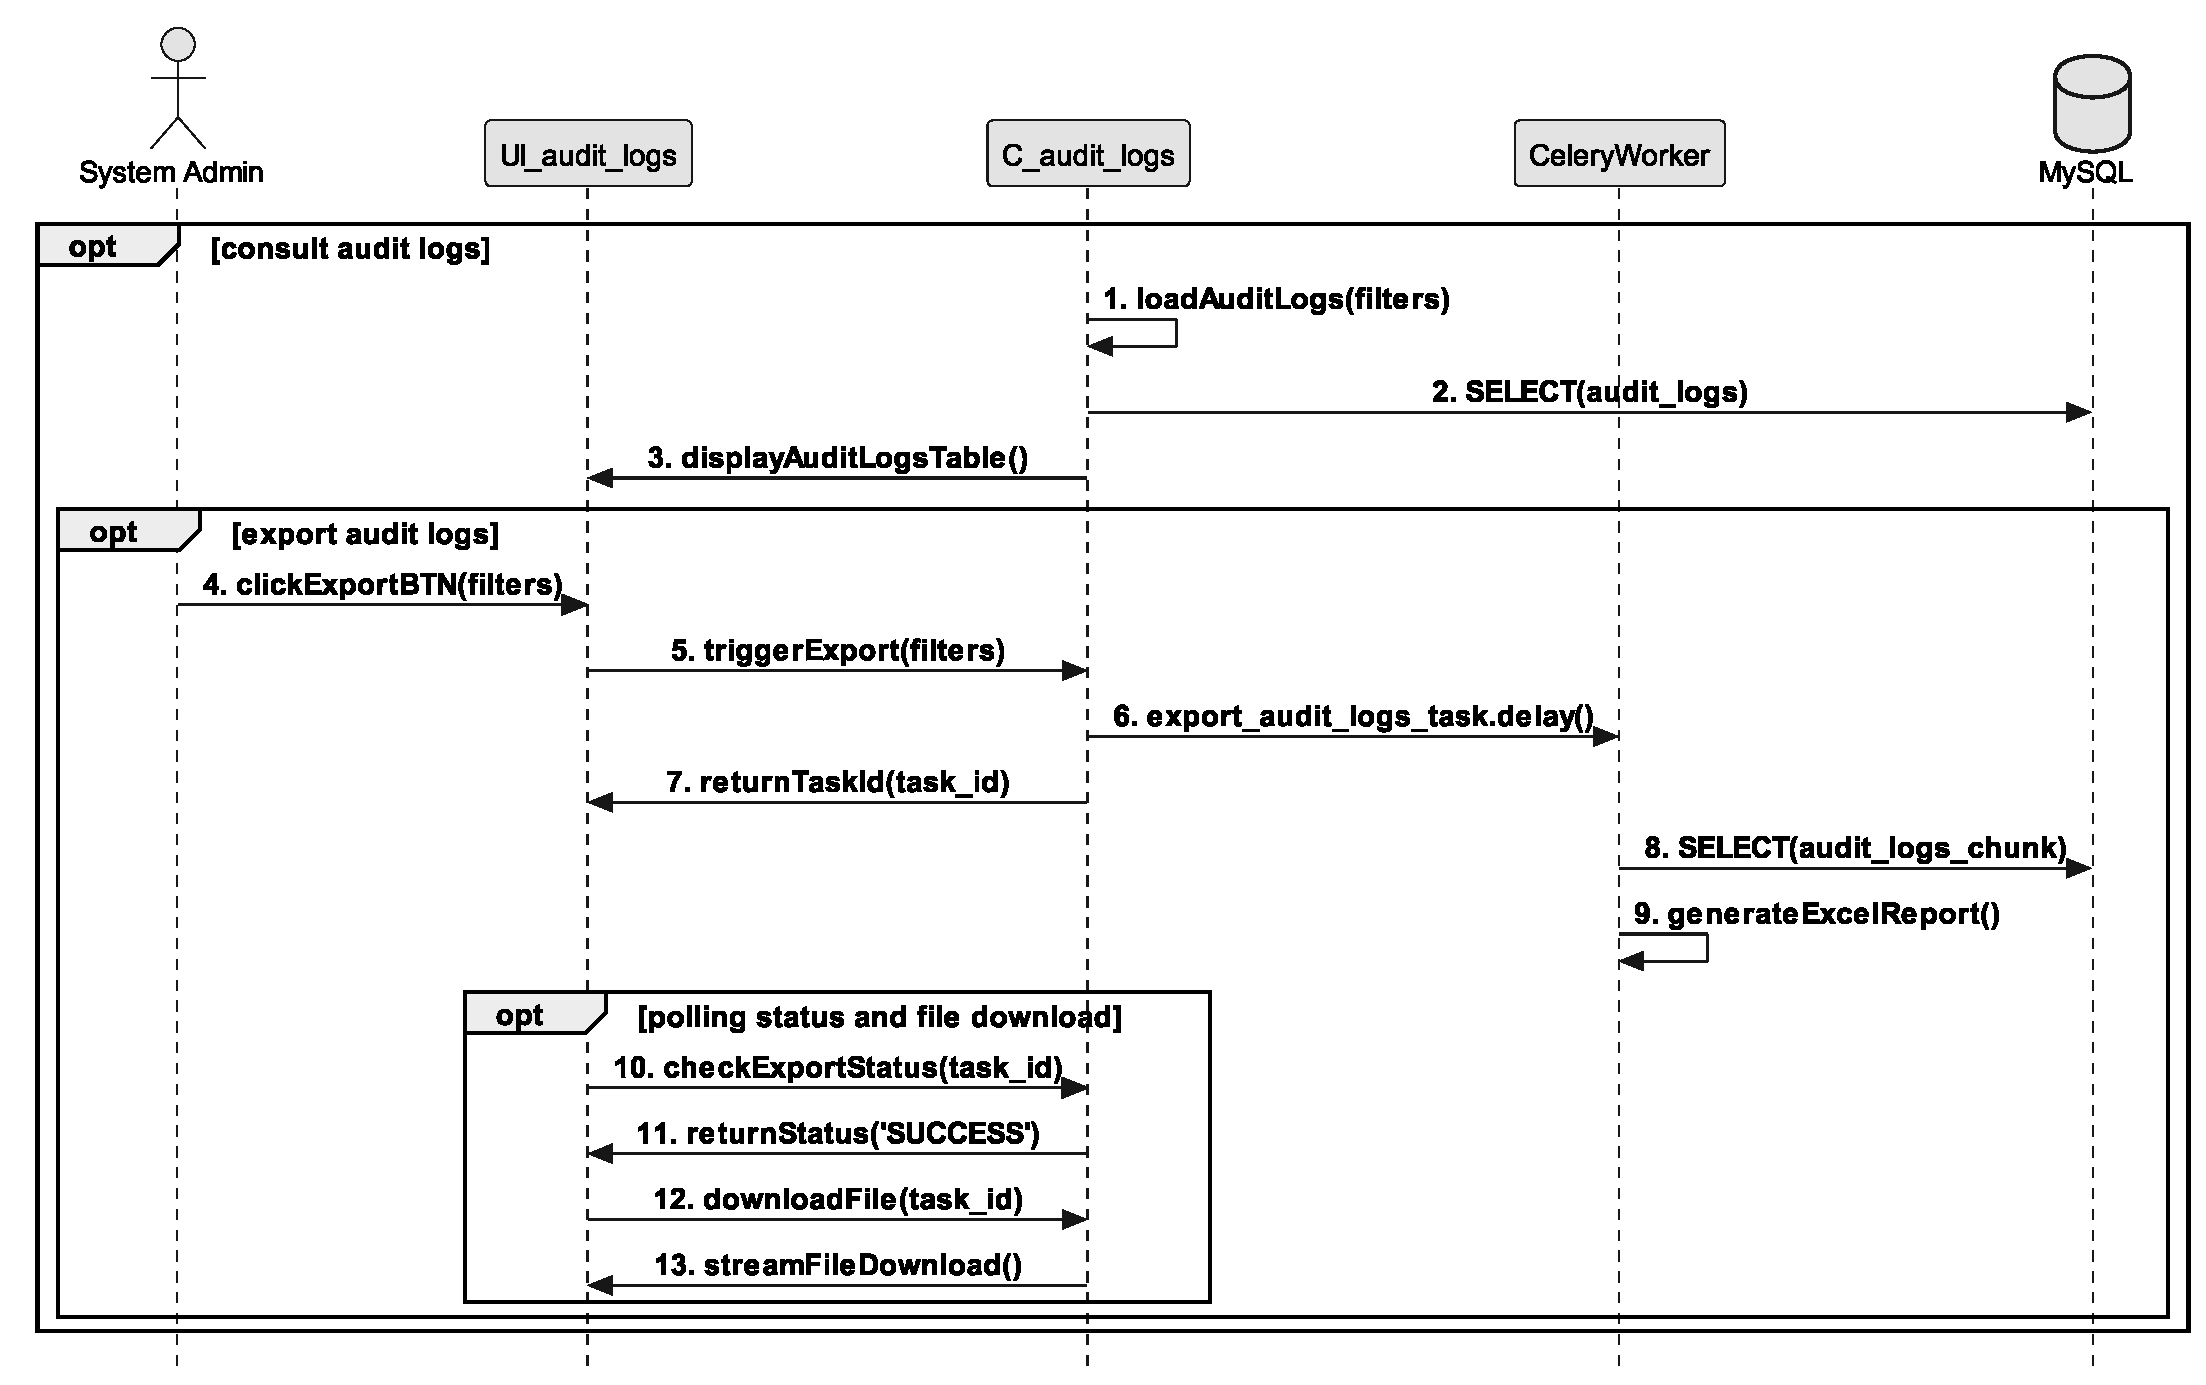
\includegraphics[width=1.2\textwidth]{images/out/diagrams/seq/audit_logs/audit_logs.eps}}
    \caption{Sequence Diagram -- Consult audit logs}
    \label{fig:seq_consult_audit}
\end{figure}

\newpage
\section{Sprint 2 Implementation}
This section presents the user interface implementations developed during Sprint 2.

\subsection{Consult Notifications Interface}
\begin{figure}[H]
    \centering
    \makebox[\textwidth][c]{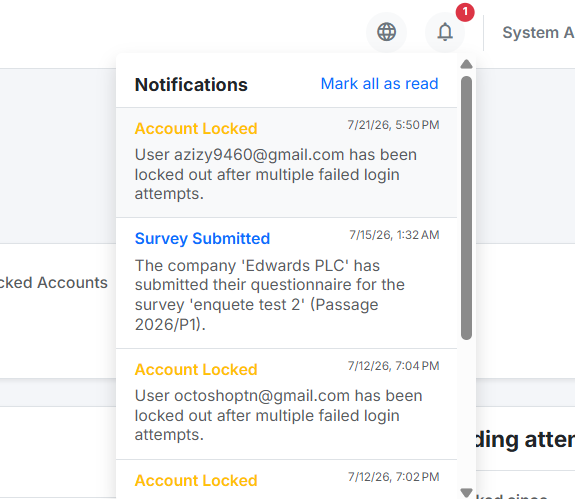
\includegraphics[width=0.5\textwidth]{images/screenshots/sprint2/notif.png}}
    \caption{Consult Notifications Interface}
    \label{fig:ui_notifications}
\end{figure}

Real-time notification delivery is powered by a dedicated WebSocket background thread connected to a Redis Pub/Sub channel (\texttt{notifications\_channel}). When an event occurs (such as survey submission or batch import completion), the service publishes a JSON payload to Redis. The WebSocket connection manager receives the payload and dispatches it asynchronously to active client connections without polling overhead. Listing \ref{lst:websocket_pubsub} presents the Redis listener implementation in the ConnectionManager.

\begin{lstlisting}[language=Python, caption={Redis Pub/Sub WebSocket Manager (\texttt{app/core/websockets.py})}, label={lst:websocket_pubsub}]
def _listen_to_redis(self):
    try:
        redis = get_redis_client()
        pubsub = redis.pubsub()
        pubsub.subscribe("notifications_channel")
        for message in pubsub.listen():
            if message["type"] == "message":
                data = json.loads(message["data"])
                uid = data.get("user_id")
                if uid and uid in self.active_connections:
                    asyncio.run_coroutine_threadsafe(
                        self.send_personal_message(data, uid),
                        self.loop
                    )
    except Exception as e:
        logger.error(f"Redis PubSub listener error: {e}")
\end{lstlisting}

\subsection{Consult Audit Logs Interface}
\begin{figure}[H]
    \centering
    \makebox[\textwidth][c]{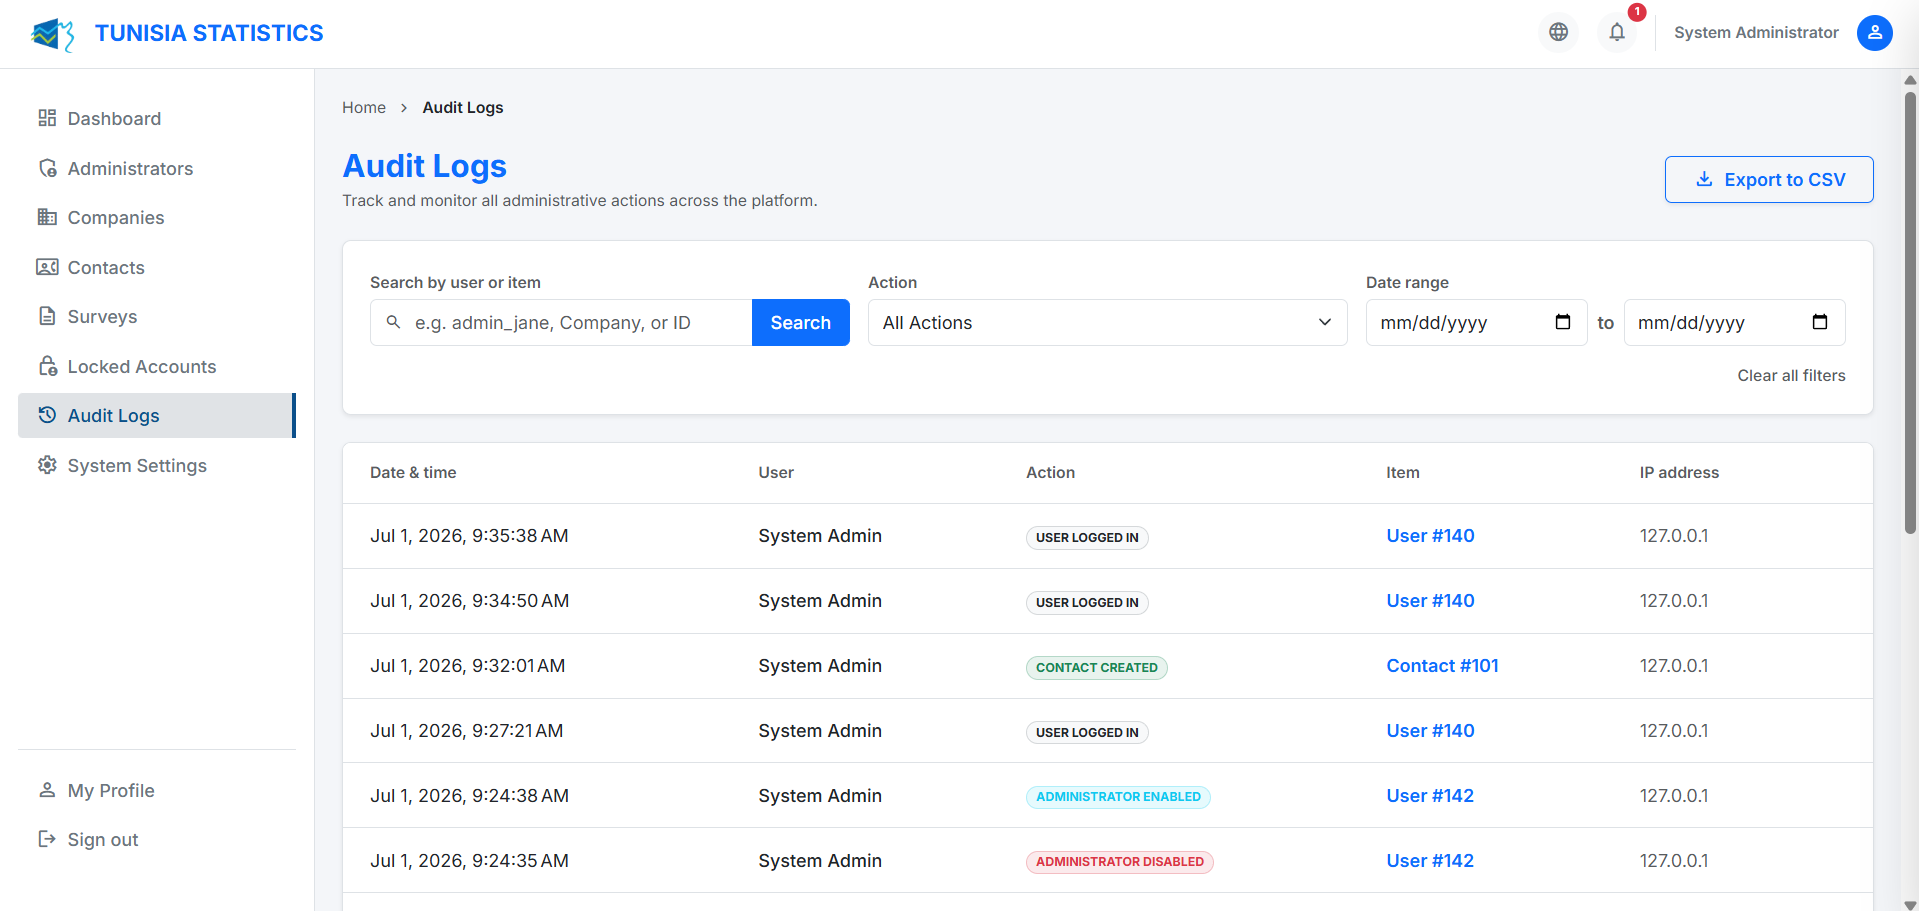
\includegraphics[width=1.1\textwidth]{images/screenshots/sprint2/audit_logs.png}}
    \caption{Consult Audit Logs Interface}
    \label{fig:ui_audit_logs}
\end{figure}

\section{Testing and System Validation}
System validation was conducted to ensure functional correctness, security enforcement, and performance stability across all platform components.

\subsection{Test Strategy}
The verification strategy comprised two complementary methodologies:
\begin{enumerate}
    \item \textbf{Manual REST API Verification:} Constructing and executing test suites using Postman \cite{postman} to validate response codes, payload structures, authentication guards, and error handling for all REST endpoints.
    \item \textbf{Synthetic Stress Testing:} Developing an automated dataset generator producing high-volume Excel files ($\approx$100MB, 500,000+ rows) to stress test the asynchronous Celery parsing pipeline, memory limits, and staging table pagination under adversarial error conditions.
\end{enumerate}

\subsection{Test Cases and Results}
Table \ref{tab:test_cases} details representative test cases executed across functional modules during system verification:

\begin{table}[H]
\centering
\caption{System Test Cases and Execution Results}
\label{tab:test_cases}
\vspace{0.2cm}
\small
\renewcommand{\arraystretch}{1.15}
\makebox[\textwidth][c]{%
\begin{tabular}{|c|p{2.5cm}|p{5.5cm}|p{5.0cm}|c|}
\hline
\textbf{ID} & \textbf{Component} & \textbf{Test Description} & \textbf{Expected Result} & \textbf{Status} \\ \hline
TC-01 & Authentication & Login with valid credentials & HTTP 200 + Redis OTP sent & PASS \\ \hline
TC-02 & Authentication & Submit invalid OTP code & HTTP 400 ``Invalid OTP'' & PASS \\ \hline
TC-03 & Security & 3 consecutive failed logins & Account locked in Redis for 24h & PASS \\ \hline
TC-04 & Security & Call protected endpoint without JWT & HTTP 401 Unauthorized & PASS \\ \hline
TC-05 & Security & Use blacklisted token after logout & HTTP 401 ``Token blacklisted'' & PASS \\ \hline
TC-06 & Admin Directory & Create admin with existing email & HTTP 400 ``Email already exists'' & PASS \\ \hline
TC-07 & RBAC Guard & Account Manager accessing Admin API & HTTP 403 Forbidden & PASS \\ \hline
TC-08 & Batch Import & Upload 100MB valid Excel sample & Async session created, rows staged & PASS \\ \hline
TC-09 & Batch Import & Upload file with missing columns & Session marked failed with error details & PASS \\ \hline
TC-10 & Batch Import & Duplicate tax ID in import file & Per-row validation error in staging & PASS \\ \hline
TC-11 & Integration & Resolve valid UUID token & HTTP 200 + Question payload & PASS \\ \hline
TC-12 & Integration & Resolve UUID for closed passage & HTTP 400 ``Passage closed'' & PASS \\ \hline
TC-13 & Integration & Resolve invalid UUID token & HTTP 404 ``Token not found'' & PASS \\ \hline
TC-14 & Notifications & Survey submission trigger & Real-time WebSocket delivery & PASS \\ \hline
TC-15 & Audit Logs & Export 50,000 audit rows & Background task generates Excel file & PASS \\ \hline
\end{tabular}%
}
\end{table}

\newpage
\subsection{Performance and Stress Test Verification}
Stress testing focused on verifying backend resilience when parsing large company sample files. Synchronous upload processing in legacy systems caused main thread blocking and browser timeouts. 

Under the new architecture, uploading a 100MB file (500,000 rows) returns an HTTP 202 response immediately with a task session ID. Celery worker threads parse the file in 2,000-row chunks using openpyxl read-only mode, keeping worker memory consumption below 50MB throughout execution. Staging rows are committed in bulk batches, and the Angular frontend polls progress with server-side pagination, maintaining fluid 60fps UI responsiveness.

\section{Sprint 2 Conclusion}
This chapter detailed the development of Sprint 2, which successfully established the real-time notification engine, systemic audit trail, and full system verification suite. All functional requirements across Sprints 0, 1, and 2 have been implemented, integrated, and validated.

\clearpage
\chapter*{General Conclusion}
\addcontentsline{toc}{chapter}{General Conclusion}
\markboth{General Conclusion}{General Conclusion}

This graduation project, conducted in collaboration with the National Institute of Statistics (INS) Tunisia, designed and implemented a web platform for administrative tracking and statistical survey collection. The platform replaces legacy paper-based workflows with a decoupled architecture, role-segmented administrative controls, asynchronous background processing, and a passwordless external access model.

Development was conducted following the Agile Scrum methodology across three functional sprints:
\begin{itemize}
    \item \textbf{Sprint 0 (Authentication \& Organization Directory):} Implemented secure authentication with 2FA OTP verification, Redis-backed rate limiting and account lockout enforcement, and company/contact directory management.
    \item \textbf{Sprint 1 (Survey Management \& Response Portal):} Developed survey passage configuration, sample mapping, company contact submission portals, and passwordless UUID token integration.
    \item \textbf{Sprint 2 (Real-Time Notifications, Auditing \& Testing):} Built an event notification engine using Redis Pub/Sub and WebSockets, systemic audit logging with asynchronous Excel export via Celery, and performed end-to-end system testing.
\end{itemize}

From an engineering perspective, the platform decouples UI, business logic, persistence, and background tasks: an \textbf{Angular} single-page application frontend, a \textbf{FastAPI} backend, a \textbf{MySQL} database, and a \textbf{Redis + Celery} task worker infrastructure.

\section*{Architectural Challenges and Lessons Learned}
During system development, key technical challenges were identified and addressed:
\begin{enumerate}
    \item \textbf{Main API Freezing on Heavy File Operations:} Initial tests showed that synchronous parsing of 100MB Excel company samples blocked FastAPI's main event loop, causing API timeouts for concurrent users. This was solved by offloading parsing to background Celery tasks, writing validated rows to a \texttt{company\_import\_staging} table, and serving the frontend via server-side pagination.
    \item \textbf{Single-Threaded Worker Bottlenecks:} Running Celery with a single thread caused small background tasks to queue behind multi-minute file imports. Increasing concurrency via threaded worker pools (\texttt{-P threads -c 4}) allowed small tasks to execute concurrently alongside heavy imports.
    \item \textbf{Token Revocation on Logout:} JWT tokens are stateless by default. Immediate access revocation was achieved by storing a unique \texttt{jti} claim in Redis on logout, checked by the authentication dependency guard on every request.
\end{enumerate}

\section*{System Limitations}
The current implementation has two main operational limitations:
\begin{enumerate}
    \item \textbf{External Questionnaire Engine Dependency:} The questionnaire filling interface is rendered by an external application linked via UUID tokens. While this decouples survey form rendering, it requires maintaining server-to-server API key synchronization.
    \item \textbf{Single-Node Redis Broker:} In the development environment, Redis operates as a single instance. Production deployment requires configuring a Redis Sentinel cluster for high availability and failover.
\end{enumerate}

\section*{Perspectives and Future Work}
Future enhancements planned for the platform include:
\begin{enumerate}
    \item \textbf{Automated CI/CD Pipeline:} Integrating automated GitHub Actions pipelines for running unit test suites and building Docker production containers automatically on code push.
    \item \textbf{Statistical Anomaly Detection:} Implementing automated data validation rules to flag outlier responses prior to statistical aggregation.
    \item \textbf{Offline Mobile Collection App:} Developing a Progressive Web App (PWA) for field enumerators collecting offline survey responses in rural regions.
\end{enumerate}

\clearpage
\addcontentsline{toc}{chapter}{Bibliography}
\begin{thebibliography}{99}

\bibitem{ins} National Institute of Statistics (INS) Tunisia: \url{http://www.ins.tn/}, consulted on 20/07/2026.

\bibitem{angular} Angular Framework: \url{https://angular.io/}, consulted on 21/07/2026.

\bibitem{fastapi} FastAPI Framework: \url{https://fastapi.tiangolo.com/}, consulted on 21/07/2026.

\bibitem{python} Python Language: \url{https://www.python.org/}, consulted on 22/07/2026.

\bibitem{celery} Celery Task Queue: \url{https://docs.celeryq.dev/}, consulted on 22/07/2026.

\bibitem{redis} Redis Data Store: \url{https://redis.io/}, consulted on 23/07/2026.

\bibitem{docker} Docker Container Platform: \url{https://www.docker.com/}, consulted on 23/07/2026.

\bibitem{scrum} K. Schwaber and J. Sutherland: The Scrum Guide, \url{https://scrumguides.org/}, consulted on 24/07/2026.

\bibitem{vscode} Visual Studio Code IDE: \url{https://code.visualstudio.com/}, consulted on 24/07/2026.

\bibitem{git} Git Version Control: \url{https://git-scm.com/}, consulted on 25/07/2026.

\bibitem{github} GitHub Repository Hosting: \url{https://github.com/}, consulted on 25/07/2026.

\bibitem{postman} Postman API Platform: \url{https://www.postman.com/}, consulted on 26/07/2026.

\bibitem{plantuml} PlantUML Modeling Tool: \url{https://plantuml.com/}, consulted on 26/07/2026.

\bibitem{overleaf} Overleaf Online LaTeX Editor: \url{https://www.overleaf.com/}, consulted on 27/07/2026.

\bibitem{mysql} MySQL Database System: \url{https://www.mysql.com/}, consulted on 27/07/2026.

\bibitem{sqlite} SQLite Database Engine: \url{https://www.sqlite.org/}, consulted on 28/07/2026.

\bibitem{sqlalchemy} SQLAlchemy ORM: \url{https://www.sqlalchemy.org/}, consulted on 28/07/2026.

\bibitem{ngx_translate} NGX-Translate Internationalization Library: \url{https://ngx-translate.org/}, consulted on 29/07/2026.

\bibitem{loi9932} Loi n° 99-32 du 13 avril 1999, relative au système national de la statistique, Journal Officiel de la République Tunisienne, \url{https://www.ins.tn/sites/default/files/loi%20n%C2%B099-32%20du%2013avril%201999,%20relatif%20au%20syst%C3%A8me%20national%20de%20la%20statistique%20link%208_0.pdf}, consulted on 29/07/2026.

\bibitem{odk} Open Data Kit (ODK): \url{https://getodk.org/}, consulted on 30/07/2026.

\bibitem{kobotoolbox} KoboToolbox Data Collection Tool: \url{https://www.kobotoolbox.org/}, consulted on 31/07/2026.

\bibitem{limesurvey} LimeSurvey Online Survey Tool: \url{https://www.limesurvey.org/}, consulted on 01/08/2026.

\bibitem{sommerville} I. Sommerville: \textit{Software Engineering}, 10th ed., Pearson, 2015.

\bibitem{fielding} R. T. Fielding: \textit{Architectural Styles and the Design of Network-based Software Architectures}, Doctoral dissertation, University of California, Irvine, 2000.

\bibitem{rfc7519} M. Jones, J. Bradley, N. Sakimura: \textit{JSON Web Token (JWT)}, RFC 7519, IETF, 2015.

\bibitem{gamma} E. Gamma, R. Helm, R. Johnson, J. Vlissides: \textit{Design Patterns: Elements of Reusable Object-Oriented Software}, Addison-Wesley, 1994.

\bibitem{rfc4122} P. Leach, M. Mealling, R. Salz: \textit{A Universally Unique IDentifier (UUID) URN Namespace}, RFC 4122, IETF, 2005.

\end{thebibliography}

\end{document}
